\documentclass[9pt]{article} 
\usepackage[utf8]{inputenc}
\usepackage[a4paper,top=2cm, bottom=2cm, outer=6cm, inner=2cm, heightrounded, marginparwidth=5cm, marginparsep=1cm]{geometry}
\usepackage{graphicx}
%\usepackage{blindtext}
\usepackage{marginnote}
\usepackage{multirow}
\usepackage{diagbox}
\usepackage{mhchem}
\usepackage{url}
\usepackage{subfigure}
\usepackage{amsfonts,latexsym} % para tener disponibilidad de diversos simbolos
\usepackage{enumerate}
%\usepackage{booktabs}
\usepackage{float}
%\usepackage{threeparttable}
\usepackage{array,colortbl}
%\usepackage{ifpdf}
\usepackage{longdivision}
\usepackage{polynom}
%\usepackage{rotating}
\usepackage{cite}
\usepackage{stfloats}
\usepackage{url}
\usepackage{listings}
\usepackage{fancyhdr}
\usepackage{makeidx}
\usepackage{color}
\usepackage{hyperref}
\hypersetup{
    colorlinks=true, %set true if you want colored links
    linktoc=all,     %set to all if you want both sections and subsections linked
    linkcolor=CarnationPink,  %choose some color if you want links to stand out
}
%\usepackage{wrapfig}
\usepackage{array}
\usepackage[symbol]{footmisc}
%\usepackage{multirow}
%\usepackage{adjustbox}
%\usepackage{nccmath}
% BOXES 
\usepackage{tikz}
\usepackage[most]{tcolorbox}
\tcbset{blue box/.style={
    enhanced, fonttitle=\bfseries,
    colback=white, colframe=accdarklight,
    coltitle=white, colbacktitle=accdark,
    attach boxed title to top left={xshift=0.3cm,
                                    yshift*=-\tcboxedtitleheight/2},
    boxed title style={
      before upper=\hspace*{0.5cm}, % reserve space for the image
      overlay={
       \node at ([xshift=0.5cm]frame.west) {};
        
      }
    }
  }
}
\newtcolorbox{mybox}[1][]{blue box, #1}
\usepackage{amsmath}
\usepackage{amssymb}
\usepackage[dvipsnames]{xcolor}


\newcommand{\titulo}{Aufarbeitung Diskrete Mathematik}
\newcommand{\nombre}{Lil'Jana}
\newcommand{\FCE}{\textbf{WiSe 2024/2025} und \textbf{WiSe 2025/2026}}
\newcommand{\resumen}{Abstrakt}


% Glossary 
\usepackage[automake]{glossaries}
\newglossary*{dinge}{Was ist was?}
\glsaddkey
 {formB}
 {}
 {\glsentryB}
 {\GlsentryB}
 {\glsB}
 {\GlsB}
 {\GLSB}
 \glsaddkey
 {formF}
 {}
 {\glsentryF}
 {\GlsentryF}
 {\glsF}
 {\GlsF}
 {\GLSF}
\makeglossaries
\loadglsentries{gloss} 

\newcommand{\charfunc}[1]{\glsentrytext{charfunc} mit $A = #1$, also $\chi_{#1}$}


% Index
\usepackage{imakeidx}
\makeindex




\usepackage{fancyhdr}
\pagestyle{fancy}
\fancyhead{}
\fancyfoot{}
\fancyhead[LO]{\small\nombre}
\fancyhead[RE]{\small\titulo}
\fancyhead[LO]{\small\FCE}
\fancyfoot[RO,LE] {\thepage}

\setcounter{page}{1} %Número de la página, la editorial lo cambiará


\newcommand{\mapsfrom}{\mathrel{\style{display:inline-block; transform:scale(-1,1);}{\mapsto}}}
\newcommand{\X}{$X$}
\usepackage{amsthm}
%\theoremstyle{definition}
\newtheoremstyle{mytheoremstyle} % name
    {\topsep}                    % Space above
    {\topsep}                    % Space below
    {}                   % Body font
    {}                           % Indent amount
    {\bfseries}                   % Theorem head font
    {}                          % Punctuation after theorem head
    {1.5em}                       % Space after theorem head
    {\thmname{#1}\thmnumber{ #2}\thmnote{ #3}}  % Theorem head spec (can be left empty, meaning ‘normal’)

\theoremstyle{mytheoremstyle}
\newtheorem{bsp}{Beispiel}[section]
\newtheorem{info}[bsp]{Zusatzinformation}
\newtheorem{reg}[bsp]{Regel}
\newtheorem{satz}[bsp]{Satz}
\newtheorem{lem}[bsp]{Lemma}
\newtheorem{defi}[bsp]{Definition}
\newtheorem{fr}[bsp]{Frage}
\newtheorem{beo}[bsp]{Beobachtung}
\newtheorem{prinz}[bsp]{Prinzip}
\newtheorem{bem}[bsp]{Bemerkung}
\newtheorem{anmerkung}{Anmerkung}[]
\newtheorem{folg}[bsp]{Folgerung}
\newtheorem{er}[bsp]{Erinnerung}
\newtheorem{prob}[bsp]{Problem}
\newtheorem{eig}[bsp]{Eigenschaften}
\newcommand{\anm}[2]{
\color{Blue} \noindent
\begin{anmerkung}  \textit{zu "#1"}  \newline
#2
\end{anmerkung} \color{black}
}

\newcommand{\regel}[2]{
\begin{reg} \textbf{#1}  \newline
#2
\end{reg}
}
\newcommand{\prin}[2]{
\begin{prinz} \textbf{#1}  \newline
#2
\end{prinz}
}
\newcommand{\rsp}[3]{
\noindent \textbf{#1} \pageref{rsp:#2}  

\noindent #3 

}
\newcommand{\stz}[3]{
\noindent \textbf{#1} \pageref{satz:#2}  

\noindent #3 

}
\newcommand{\txc}[1]{
\textcolor{Blue}{#1}
}
\newcommand{\za}[1]{\mathbb{Z} / #1 \mathbb{Z}}
\newcommand{\zat}[0]{\mathbb{Z} / m \mathbb{Z}}
\newcommand{\zatx}[1]{\mathbb{Z} / #1 \mathbb{Z}[x]}
\usepackage[onehalfspacing]{setspace} 
\renewcommand{\thefootnote}{\roman{footnote}}


\newcommand{\explainvkr}[0]{\footnote{$v$: Anzahl der Elemente in der Menge $X$} \footnote{$k$: Anzahl der Elemente pro Block} \footnote{$r$: in wie vielen Blöcken ein Element vorkommen soll}}
\newcommand{\explainvkrb}[0]{\explainvkr \footnote{$b$: Anzahl der Blöcke im Design}}
\newcommand{\explaindesign}[0]{\footnote{$\mathcal{B}, \mathcal{C}, ...$: damit sind Designs gemeint}}
\newcommand{\explainrs}[0]{\footnote{$r_s, r_t, ...$: t bzw. s ist die Größe der Teilmengen von X, die gleich oft in allen $r_t$ Blöcken eines $t$-Designs vorkommen soll}}

\newcommand{\bluenote}[1]{\marginpar{\textcolor{Blue}{#1}}}
\begin{document}



\tableofcontents
\newpage 
\section*{Legende}
\begin{tabular}{ll}
    Skript & normale schwarze Schrift  \\
    Anmerkungen und Notizen  & \txc{Blaue Schrift} 
\end{tabular}
\let\thefootnote\relax\footnote{Footnotes have no numbers}
\newpage
\section*{Einführung} 
Diskrete Mathematik wie Kombinatorik und Graphentheorie erlebt einen
rasanten Anstieg von Anwendungen in der Bioinformatik. Graphen werden
benutzt um Netzwerke und biologische Phänomene darzustellen. Um diese
zu studieren werden neue Methoden der Graphentheorie entwickelt. Algebraische Methoden der diskreten Mathematik wie erzeugende Funktionen finden
Einsatz um sogenannte ‘Riesenkomponenten’ von Netzwerken zu bestimmen.
Ringtheorie wird angewendet um neuronale Codes zu studieren. Oft kommt
es zu enormen Datenmengen wie zum Beispiel in der Genomforschung. Da
braucht es fehlerkorrigierende Codes.
\chapter{Vorlesungsinhalte}
\section{Elementare Zählprinzipien}
\subsubsection*{Vorlesung 1 - 11.10.2024}
\addcontentsline{toc}{subsection}{Vorlesung 1}
 Wir betrachten endliche Mengen. Für eine solche Menge \X , sei $|X|$ die Anzahl deren Elemente. Dies wird auch die \textit{Mächtigkeit} oder \textit{Kardinalität} von \X \ genannt.  
 
\regel{Summenregel}{
 Sind die Mengen $X_1, . . . , X_n$ \gls{paarweise disjunkt}, so gilt \[\left| X_1 \cup X_2 \cup \dots \cup X_n \right| = \left| X_1 \right| + \cdots + \left| X_n \right| = \sum_{i=1}^{n} \left| X_i \right|.\] 
  \txc{Also: Die Anzahl der Elemente in der Vereinigung aller Mengen ist gleich die Summe der Anzahl der Elemente in jeder der Mengen.} \label{rsp:summenregel}}
\anm{paarweise disjunkt}{
Ein Mengensystem $M$, also eine Menge von Mengen, nennt man \gls{paarweise disjunkt}, wenn jeweils zwei verschiedene Mengen $A, B \in M$ disjunkt sind.
}

\begin{bsp}
Eine Schule besitzt die Klassen $K_1, K_2, \dots, K_{18}$. Dann gibt es insgesamt \[\sum_{i=1}^{18} |K_i|\] Schüler und Schülerinnen. \\
Das \textit{kartesische Produkt} $X \times Y$ von zwei Mengen $X$, $Y$ besteht aus den geordneten Paaren $(x, y)$, wobei $x \in X$, $y \in Y$. Allgemeiner definiert man das Produkt $X_1 \times X_2 \times \cdots \times X_n$ als die Menge der $n$-Tupel $(x_1, \dots, x_n)$ mit $x_i \in X_i$ für alle $i$.
\end{bsp} \noindent \rule{8cm}{0.4pt} 

\regel{Produktregel}{$\left| X_1 \times X_2 \times \cdots \times X_n \right| = \left| X_1 \right| \cdot \cdots \cdot \left| X_n \right| = \prod_{i=1}^{n} \left| X_i \right|.$ \label{rsp:produktregel} }
\anm{Produktregel}{Man kann die Produktregel auch so formulieren: Falls für eine endliche Menge $M = M_1 \times \cdots \times M_k$ ist (sie aus dem kartesischen Produkt all ihrer Teilmengen besteht), so gilt: 
\[\mid M \mid = \prod^k_{i=1} \mid M_i \mid \]
}


\begin{bsp}
Auf einer Speisekarte gibt es 2 Vorspeisen, 4 Hauptgerichte und 3 Nachspeisen. Dann gibt es 
$2 \cdot 4 \cdot 3 = 24$ 
verschiedene Drei-Gänge-Menüs. \\
Sind alle Mengen $X_i$ dieselbe Menge $X$, so bezeichnen wir die Menge $X \times \cdots \times X$ der $n$-Tupel von Elementen in $X$ auch mit $X^n$. Die Produktregel liefert:
\end{bsp} \noindent \rule{8cm}{0.4pt}

\regel{Potenzregel}{$\left| X^n \right| = \left| X \right| \cdot \cdots \cdot \left| X \right| = \left| X \right|^n
$  \label{rsp:potenzregel}}

\begin{bsp}
Eine Kreditkarten PIN besteht aus 4 Ziffern. Es gibt $10^4 =
10000$ mögliche PINs.
\end{bsp} \noindent \rule{8cm}{0.4pt}

\begin{bsp}
Die Anzahl Wörter der Länge $n$ in einem Alphabet $X$ mit $m$ Buchstaben ist
$\left| X^n \right| = m^n$. \\
Die Kardinalität von $X^n$ ist also die Anzahl von Möglichkeiten bei einer \textit{geordneten} Auswahl von $n$ Elementen aus $X$ mit Zurücklegen (bzw. mit Wiederholung). \\
Bei der \textit{geordneten} Auswahl \textit{ohne} Wiederholung wollen wir eine Liste von $n$ Einträgen ohne Wiederholung aus einer Menge mit $m$ Elementen zusammenstellen. Dazu gibt es
$m(m - 1) \cdot \dots \cdot (m - n + 1)$ Möglichkeiten.
\end{bsp} \noindent \rule{8cm}{0.4pt} 

\begin{bsp}
Wenn man eine PIN selber festlegt, wählt man häufig vier verschiedene Ziffern. Es gibt
$10 \cdot 9 \cdot 8 \cdot 7 = 5040$
Möglichkeiten für eine PIN aus verschiedenen Ziffern.
\end{bsp} \noindent \rule{8cm}{0.4pt}

\begin{bsp}
Bei einer Lotto-Ziehung 6 aus 49 gibt es
$49 \cdot 48 \cdot 47 \cdot 46 \cdot 45 \cdot 44$
Möglichkeiten. \\
Ein $n$-Tupel $(a_1, a_2, \dots, a_n) \in X^n$ können wir auch als Funktion von $\{1, \dots, n\}$ nach $X$ auffassen:
\[
\{1, \dots, n\} \to X, \quad i \mapsto a_i.
\]
Diese ist genau dann injektiv, wenn im Tupel keine Wiederholung vorkommt. Somit gilt:
\end{bsp} \noindent \rule{8cm}{0.4pt}


\begin{satz} \label{satz1-8}
\textit{Sei $N$ eine Menge mit $n$ Elementen und $X$ eine Menge mit $m$ Elementen. \\
Dann gibt es $m^n$ Abbildungen $N \to X$ und $m(m - 1) \cdot \dots \cdot (m - n + 1)$ injektive Abbildungen $N \to X$.
} \\
\txc{
Für die injektive Abbildung kann man wie folgt argumentieren:
\begin{itemize}
    \item \textbf{Erstes Element:} Für das erste Element aus $N$ gibt es $m$ Möglichkeiten, es in $X$ abzubilden.
    \item \textbf{Zweites Element:} Für das zweite Element gibt es $m - 1$ Möglichkeiten, da es nicht auf das Element abgebildet werden kann, das bereits vom ersten Element gewählt wurde.
    \item \textbf{Drittes Element:} Für das dritte Element gibt es $m - 2$ Möglichkeiten, und so weiter.
    \item \textbf{n-tes Element:} Für das $n$-te Element gibt es schließlich $m - (n - 1)$ Möglichkeiten, weil bereits $n - 1$ Elemente aus $X$ belegt sind.
\end{itemize}
Die Anzahl der injektiven Abbildungen ist also: \\
$
m \cdot (m - 1) \cdot (m - 2) \cdots (m - (n - 1)) \\ = m(m - 1)(m - 2) \cdots (m - n + 1).
$
}
 \end{satz} \noindent \rule{8cm}{0.4pt}

\regel{Gleichheitsregel}{Für Mengen $X$, $Y$ gilt $\left| X \right| = \left| Y \right|$ genau dann, wenn es eine Bijektion $X \to Y$ gibt. \\
Falls es also eine Bijektion zwischen $X$ und $Y$ gibt, dann können wir die Kardinalität von $X$ mittels der Kardinalität von $Y$ berechnen.
\label{rsp:gleichheitsregel}} 


\begin{bsp}
Es gibt eine Bijektion zwischen den Teilmengen von $X$ und den Abbildungen $X \to \{0, 1\}$. Einer Teilmenge $A \subseteq X$ wird die charakteristische Funktion
\[
\glspl{chiA}_A: X \to \{0, 1\}, \quad x \mapsto 
\begin{cases} 
0, & x \notin A \\
1, & x \in A 
\end{cases}
\]
zugeordnet. Somit ist die Anzahl der Teilmengen von $X$ gleich der Anzahl der Funktionen $X \to \{0, 1\}$, also $2^{|X|}$.

Man kann die Gleichheitsregel auch nutzen, um zu zeigen, dass zwei Mengen gleich groß sind, wenn man deren Anzahl von Elementen nicht explizit bestimmen kann. Das Anwenden der folgenden Zählregel ist für uns wichtiger als ihre abstrakte Formulierung. Deshalb betrachten wir zunächst ein Beispiel.

\end{bsp} \noindent \rule{8cm}{0.4pt} 

\begin{bsp}

In den Neurowissenschaften interessiert man sich für Nervenbahnen von sogenannten Neuronen vom Typ A zu Neuronen vom Typ B. In einem Modell gibt es 3 Neuronen $\{a_1, a_2, a_3\}$ vom Typ A und 5 Neuronen $\{b_1, \ldots, b_5\}$ vom Typ B. Die Matrix
 
\[
\begin{array}{c|ccccc}
    & b_1 & b_2 & b_3 & b_4 & b_5 \\
\hline
a_1 & 0 & 1 & 0 & 0 & 0 \\
a_2 & 1 & 0 & 1 & 0 & 1 \\
a_3 & 1 & 1 & 0 & 0 & 1 \\
\end{array}
\]

beschreibt, zwischen welchen Neuronen es eine Nervenbahn gibt. Die Gesamtanzahl der Nervenbahnen ist

\[
2 + 2 + 1 + 0 + 2 = 7
\]

indem wir die Spaltensummen bilden und diese addieren. Sie kann aber auch durch Addieren der Zeilensummen

\[
1 + 3 + 3 = 7
\]

berechnet werden.
Wir formalisieren dies in der folgenden Regel zur Berechnung der Kardinalität einer Teilmenge $S \subseteq X \times Y$. Für $y \in Y$ setze die 'Spaltensumme'
\[
s_y = \left| \{ x \in X \,|\, (x, y) \in S \} \right|,
\]
also die Anzahl von $x \in X$ mit $(x, y) \in S$. Für $x \in X$ setze die 'Zeilensumme'
\[
z_x = \left| \{ y \in Y \,|\, (x, y) \in S \} \right|.
\]
\end{bsp} \noindent \rule{8cm}{0.4pt}



\regel{Regel vom zweifachen Abzählen}{\[
|S| = \sum_{y \in Y} s_y = \sum_{x \in X} z_x.
\]

Das folgende Zählprinzip wird oft verwendet, um zu zeigen, dass es in einer Menge ein Element gibt mit einer gewissen Eigenschaft, ohne herauszufinden, um welches Element es sich handelt. \\
\txc{Verwendung: die Anzahl der Elemente in einer Menge zu zählen, indem man zwei unterschiedliche Wege der Zählung vergleicht. \\
Formel: Gesamtanzahl der Elemente in der Menge $S$ = Summe der Elemente in $S$, die zu einem bestimmten Element $y$ in $Y$ gehören = Summe der Elemente in $S$, die zu einem bestimmten Element $x$ in \X gehören.
} \label{rsp:zweifach}
}
\anm{Regel vom zweifachen Abzählen}{Daraus ergibt sich: Ist $A = (a_{ij})_{1 \leq i\leq m, 1\leq j \leq n}$ eine Matrix, so gilt 
\[
\sum^m_{i=1} \big( \sum^n_{j=1} a_{ij} \big) = \sum^n_{i=1} \big( \sum^m_{j=1} a_{ij} \big)
\]
d.h. die Summe der Zeilensummen ist gleich der Summe der Spaltensummen. \footnote{https://www.math2.rwth-aachen.de/files/dmve/notizen/Skript.pdf}
}
\color{Blue}
\begin{bsp}
Angenommen, wir haben eine Klasse von 30 Studenten, von denen 15 Mathematik und 12 Informatik studieren. Wir möchten wissen, wie viele Studenten mindestens eines der beiden Fächer studieren.
Sei 
\[
s_{\text{Mathematik}} = 15
\]
\[
s_{\text{Informatik}} = 12
\]
Dann gilt 
\[
|S| = s_{\text{Mathematik}} + s_{\text{Informatik}} = 15 + 12 = 27.
\]
Nun zählen wir die Studenten nach dem, was sie studieren:
\begin{itemize}
    \item Anzahl der Studenten, die Mathematik studieren: $15$
    \item Anzahl der Studenten, die Informatik studieren: $12$
    \item Anzahl der Studenten, die beide Fächer studieren: $x$
\end{itemize}
Die Gleichung lautet also:
\[
|S| = 15 + 12 - x
\]
Hier subtrahieren wir $x$, da diese Studenten in beiden Zählungen doppelt gezählt wurden. Setzen wir die beiden Zählungen gleich, erhalten wir:
\[
27 = 15 + 12 - x
\]
Somit ergibt sich:
\[
x = 15 + 12 - 27 = 0
\]
Das bedeutet, dass es keine Studenten gibt, die beide Fächer studieren.

\end{bsp} \noindent \rule{8cm}{0.4pt} \color{black}

\prin{Schubfachprinzip}{Verteilt man $m$ Gegenstände auf $n$ Fächer, wobei $m > n$ \txc{(also wenn es mehr Gegenstände als Fächer gibt)}, so gibt es ein Fach mit mehr als einem Gegenstand. Umformuliert besagt das Schubfachprinzip, dass es keine injektive Abbildung $X \to Y$ gibt, falls $\left| X \right| > \left| Y \right|$.
\label{rsp:schubfachprinzip} } 

\begin{figure}[H]
\color{Blue}
    \centering
    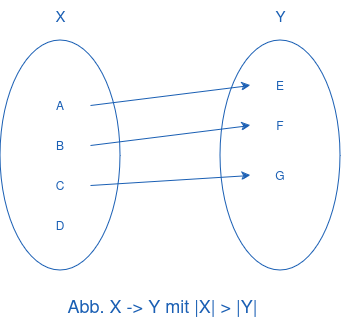
\includegraphics[width=5cm]{image/nicht_injektiv.png}
    \caption{Hier kann man sehen, wieso es eine injektive Abbildung  $X \to Y$ gibt, falls $\left| X \right| > \left| Y \right|$.}
    \label{fig:nicht_injektiv}
\end{figure}

\begin{bsp}
Kann man aus $n$ ganzen Zahlen $\{a_1, \ldots, a_n\}$ eine Teilmenge auswählen, deren Summe durch $n$ teilbar ist? Verteilen wir die $n + 1$ Zahlen $0, a_1, a_1 + a_2, \ldots, a_1 + \cdots + a_n$ auf die $n$ Zahlen $\{0, 1, \ldots, n-1\}$, indem wir deren Reste modulo $n$ berechnen, so muss es nach dem Schubfachprinzip $k < l$ geben, sodass

\[
a_1 + \cdots + a_k \equiv a_1 + \cdots + a_l \mod n.
\]

Also teilt $n$ die Differenz dieser beiden Summen: 

\[
a_{k+1} + \cdots + a_l.
\]
\color{Blue}
Nehmen wir an, dass $n = 3$ und nd die Folge der $a_i$ Zahlen sei $0, a_1=2,\ a_1 + a_2=2+3=5,\ a_1 + a_2 + a_3=2+3+4=9$. \newline
Also: $0,\ 2,\ 5,\ 9$. \newline
Es gibt n+1, also hier 4 Zahlen in der Reihe. \\ \newline
Wenn wir nun jede Zahl der Reihe modulo n berechnen, sieht das so aus: 
\begin{align*}
    \text{0 mod 3} & = 0 \\
    \text{2 mod 3} & = 2 \\
    \text{5 mod 3} & = 2 \\
    \text{9 mod 3} & = 0 
\end{align*}
Da wir $n+1=4$ Zahlen (Gegenstände) haben, die auf $n=3$ mögliche Werte (Fächer) $\{0,1,2\}$ abgebildet werden, garantiert das Schubfachprinzip, dass mindestens zwei dieser Reste identisch sein müssen (mindestens zwei der Gegenstände im gleichen Fach liegen müssen). \\ \newline
Wichtig: mit 
\[ a_1 + \cdots + a_k  \equiv a_1 + \cdots + a_l  \mod n \] ist gemeint: 
\[ (a_1 + \cdots + a_k \mod n) \equiv (a_1 + \cdots + a_l \mod n) \] 
Wählt man nun $k = 1$ und $l = 2$ aus (da der Rest 2 bei den Teilsummen $a_1$ und $a_1+a_2$ auftritt und man so die Bedingung erfüllt), würde man die Formel so ausschreiben: 
\begin{align*}
    a_1 + \cdots + a_k \mod n &  \equiv a_1 + \cdots + a_l  \mod n \\
    a_1 \mod n & \equiv  a_1  + a_2 \mod n \\
    2 \mod 3 & \equiv 2+3 \mod 3 \\
    2 \mod 3 & \equiv 5 \mod 3 \\
    2 & \equiv 2 
\end{align*}
Also teilt n (hier: 3) die Differenz beider Summen. 
\color{black}
\end{bsp} \noindent \rule{8cm}{0.4pt}


\prin{Verallgemeinertes Schubfachprinzip}{Verteilt man $m$ Gegenstände auf $n$ Fächer, wobei $m > nk$, so gibt es ein Fach mit mehr als $k$ Gegenständen.
\label{rsp:allg-schubfachprinzip}
}

\begin{bsp}
Unter 6 Menschen gibt es drei, die sich schon begegnet sind, oder drei, die sich noch nie begegnet sind. Denn fixieren wir eine Person $A$, dann gibt es drei Personen $B$, $C$, $D$, die ihr schon begegnet sind, oder drei Personen $B$, $C$, $D$, die ihr noch nicht begegnet sind.

Wir wenden hier das verallgemeinerte Schubfachprinzip an mit $m = 5$ Personen und $n = 2$ Fächern (begegnet oder nicht). Eines der Fächer enthält dann mindestens drei Personen. Falls im ersten Fall sich zwei der drei Personen $B$, $C$, $D$ schon begegnet sind, dann formen diese zusammen mit $A$ drei Personen, die sich begegnet sind. Ansonsten sind sich $B$, $C$, $D$ nicht begegnet.

Im zweiten Fall kann genauso argumentiert werden, indem wir 'begegnet' und 'nicht begegnet' vertauschen.
\begin{figure}
\color{Blue}
    \centering
    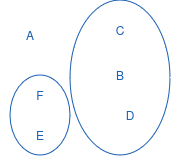
\includegraphics[width=5cm]{image/beispiel.png}
    \caption{Visualisierung der Aufteilung on zwei Gruppen.}
    \label{fig:my_label}
\end{figure}
\end{bsp} \noindent \rule{8cm}{0.4pt}

\section{Teilmengen}
In §1 haben wir eine geordnete Auswahl von $r$ Elementen aus $X$ betrachtet, also eine Liste der Länge $r$. Eine solche Liste mit (beziehungsweise ohne) Wiederholung kann man als Abbildung (beziehungsweise injektive Abbildung) $\{1, \ldots, n\} \to X$ darstellen. 

Jetzt wollen wir eine ungeordnete Auswahl betrachten. Eine ungeordnete Auswahl von $r$ Elementen aus $X$ ohne Wiederholung kann man als eine $r$-elementige Teilmenge aus $X$ darstellen.

\begin{defi}
Die Anzahl der $r$-elementigen Teilmengen einer $n$-elementigen Menge wird mit 
\[
\binom{n}{r}
\]
bezeichnet.
Insbesondere ist 
\[
\binom{n}{r} = 0 \quad \text{für } r < 0 \text{ oder } r > n.
\]
\color{Blue}
$\binom{n}{r} = 0 \quad \text{für } r < 0$, da es ist unmöglich ist eine negative Anzahl von Elementen aus einer Menge auszuwählen. Daher gibt es für diesen Fall keine sinnvolle Lösung, und der Wert wird als 0 gesetzt. \\
$\binom{n}{r} = 0 \quad \text{für } r > n$, weil man auch nicht mehr Elemente aus einer Menge auswählen kann, als die Menge besitzt.

\end{defi} \noindent \rule{8cm}{0.4pt}
\color{Blue}
\begin{bsp}
\color{Blue}
Nehmen wir als Beispiel eine Menge mit \( n = 5 \) Elementen \( \{A, B, C, D, E\} \), und wir wollen die Anzahl der Möglichkeiten berechnen, eine Teilmenge mit \( r = 2 \) Elementen zu bilden.

\[
\binom{5}{2} = \frac{5!}{2! \cdot (5 - 2)!} = \frac{5 \cdot 4 \cdot 3!}{2 \cdot 1 \cdot 3!} = \frac{20}{2} = 10
\]

Es gibt also 10 Möglichkeiten, eine 2-elementige Teilmenge aus 5 Elementen auszuwählen. Die möglichen 2-elementigen Teilmengen wären:
$
\{A, B\}, \{A, C\}, \{A, D\}, \{A, E\}, \{B, C\}, \{B, D\}, \{B, E\}, $ $\{C, D\}, \{C, E\}, \{D, E\}
$

\end{bsp} \noindent \rule{8cm}{0.4pt}
\color{black}
\begin{satz}
Für $r \leq n$ gilt
\[
\binom{n}{r} = \frac{n!}{r!(n - r)!}.
\]
\textit{Beweis.} Sei $X$ eine $n$-elementige Menge. Nach Satz 1.1. gibt es 
\[
n(n - 1) \cdots (n - r + 1) = \frac{n!}{(n - r)!}
\]
Listen von $r$ Elementen aus $X$ ohne Wiederholung. Diese Anzahl können wir auch durch 
\[
\sum_{A \subseteq X, |A| = r} | \{ \text{r-Tupel von Elementen aus } A \} |
\]
berechnen, wobei die Summe über alle $r$-elementigen Teilmengen $A$ von $X$ läuft. Da es $r!$ viele r-Tupel von Elementen aus $A$ gibt, erhalten wir
\[
n(n - 1) \cdots (n - r + 1) = \sum_{A \subseteq X, |A| = r} r! = \binom{n}{r} \cdot r!.
\]
Somit gilt
\[
\binom{n}{r} = \frac{n!}{r!(n - r)!}.
\]

 \end{satz} \noindent \rule{8cm}{0.4pt}
\color{Blue}
\begin{bsp}
\[
\binom{5}{3} = \frac{5!}{3!(5 - 3)!} = \frac{5!}{3! \cdot 2!}
\]
Und die Fakultäten: 
\[
5! = 5 \cdot 4 \cdot 3 \cdot 2 \cdot 1 = 120
\]
\[
3! = 3 \cdot 2 \cdot 1 = 6
\]
\[
2! = 2 \cdot 1 = 2
\]
Also: 
\[
\binom{5}{3} = \frac{120}{6 \cdot 2} = \frac{120}{12} = 10
\]
Gemäß der Aufgabe gibt es \(n(n - 1)(n - 2)\) Möglichkeiten, 3 Elemente aus \(X\) zu wählen und sie in einer bestimmten Reihenfolge anzuordnen:
\[
5 \cdot 4 \cdot 3 = \frac{5!}{(5 - 3)!} = \frac{120}{2} = 60 = 10 \cdot 6 = \binom{5}{3} \cdot 3!
\]
\end{bsp} \noindent \rule{8cm}{0.4pt}
\color{black}

\begin{bem}
1. Es gilt 
\[
\binom{n}{r} = \frac{n!}{r!(n-r)!} = \binom{n}{n-r}.
\]
\color{Blue}
Denn: 
\begin{align*}
    \binom{n}{r} & = \frac{n!}{r!(n-r)!}  & | \text{ per Defintion von } \binom{n}{r} \\
    & = \frac{n!}{(n - r)! \cdot r!} \\
    & =  \frac{n!}{(n - r)! \cdot (n - (n - r))!} \\
   & =  \binom{n}{n - r}  
\end{align*}
\color{black}
2. Es gilt 
\[
\sum_{r=0}^{n} \binom{n}{r} = 2^n,
\]
da diese Summe alle Teilmengen zählt. \\
\color{Blue}
Denn: 
\begin{itemize}
    \item[] \(\binom{n}{0}\) zählt die leere Menge.
    \item[] \(\binom{n}{1}\) zählt die \( n \) ein-elementigen Teilmengen.
    \item[] \(\binom{n}{2}\) zählt die \( \frac{n(n-1)}{2} \) zwei-elementigen Teilmengen.
    \item[] \(\ldots\)
    \item[] \(\binom{n}{n}\) zählt die Menge selbst als Teilmenge.
\end{itemize}
\color{black}
3. Es gibt eine Rekursion:
\[
\binom{n}{r} = \binom{n - 1}{r - 1} + \binom{n - 1}{r}.
\]
Denn fixieren wir ein Element $x \in X$, so zählt der erste Summand $r$-elementige Teilmengen $A \subseteq X$ mit $x \in A$ und der zweite Summand $r$-elementige Teilmengen $A \subseteq X$ mit $x \notin A$.
\txc{\[
\binom{n}{r} = \underbrace{\binom{n - 1}{r - 1}}_{\text{Teilmengen mit } x\in A} + \overbrace{\binom{n - 1}{r}}^{\text{Teilmengen mit } x \notin A}.
\]}
\end{bem} \noindent \rule{8cm}{0.4pt}
\begin{bsp}
Mit Hilfe des Pascalschen Dreiecks erhalten wir 
\[
\binom{7}{3} = \binom{6}{2} + \binom{6}{3} = 15 + 20 = 35.
\]
Die Ausdrücke $\binom{n}{r}$ heißen auch \textit{BinomialKoeffizient}, da sie in der binomischen Formel auftreten. Wir leiten diese her.

\end{bsp} \noindent \rule{8cm}{0.4pt}
\subsubsection*{Vorlesung 2 - 18.10.2024}
\addcontentsline{toc}{subsection}{Vorlesung 2}
\begin{satz} \label{satz2-5} \label{satz:multinomialentwicklung} \txc{allgemeine Formulierung der Multinomialentwicklung}
\[
\prod_{i=1}^n (a_i + b_i) = \sum_{I \subseteq \{1, \dots, n\}} a_I b_{I^c}, wobei ( a_I := \prod_{i \in I} a_i ).
\]
\textit{Hier bezeichnet \( I^c = \{1, \dots, n\} \setminus I \) das Komplement von \( I \), und ein Produkt über die leere Menge wird als \( 1 \) definiert.} \\
\txc{Es mischen sich nie \(a_i\) und \(b_i\) für denselben Index \(i\). Entweder wird \(a_i\) gewählt (wenn \(i \in I\)) oder \(b_i\) (wenn \(i \notin I\)). \\
Ein Term wie \(a_1 b_1\) ist daher nicht möglich, da derselbe Index \(i\) nicht gleichzeitig in \(I\) und \(I^c\) liegen kann.
}
\txc{
%\[\underbrace{\prod_{i=1}^n (a_i + b_i)}_{\text{iteratives Ausmultiplizieren aller $n$ Faktoren}}\]
\[\underbrace{\sum_{I \subseteq \{1, \dots, n\}}}_{\text{läuft über alle Teilmengen $I$ der Menge } \{1,...,n\}}\]
\[ \underbrace{a_I}_{\text{Produkt aller $a_i$, deren Indizes in $I$ enthalten}}\]
\[
\underbrace{b_I}_{\text{Produkt aller $b_i$, deren Indizes nicht in $I$ enthalten}}
\]
Von einer Darstellung als Produkt aus Summen zu einer Darstellung aus einer Summe von Produkten.  \\
}
\txc{\begin{bsp} Für $n=3$
\[
\begin{array}{|c|c|c|c|}
\hline
I & a_I & b_{I^c} & \text{Summand} \\
\hline
\emptyset & 1 & b_1 b_2 b_3 & b_1 b_2 b_3 \\
\{1\} & a_1 & b_2 b_3 & a_1 b_2 b_3 \\
\{2\} & a_2 & b_1 b_3 & a_2 b_1 b_3 \\
\{3\} & a_3 & b_1 b_2 & a_3 b_1 b_2 \\
\{1, 2\} & a_1 a_2 & b_3 & a_1 a_2 b_3 \\
\{1, 3\} & a_1 a_3 & b_2 & a_1 a_3 b_2 \\
\{2, 3\} & a_2 a_3 & b_1 & a_2 a_3 b_1 \\
\{1, 2, 3\} & a_1 a_2 a_3 & 1 & a_1 a_2 a_3 \\
\hline
\end{array}
\]
Man sieht es werden in jedem Summand alle Indizes durchlaufen - aber die Reihenfolge und Verteilung von a's und b's je Summand ist ist so angelegt, dass über die gesamte Ausrechnung der Formeln alle $2^n$ Kombinationen von a's und b's in der Summe vorkommen. 
\end{bsp} \noindent \rule{8cm}{0.4pt}}
 \end{satz} \noindent \rule{8cm}{0.4pt}
\begin{bsp}

\[
(a_1 + b_1)(a_2 + b_2) = a_1 a_2 + a_1 b_2 + a_2 b_1 + b_1 b_2.
\]

\paragraph{Beweis.} Mittels vollständiger Induktion. Die Formel gilt für \( n = 1 \): Der Summand für \( I = \{1\} \) ist \( a_1 \), und der für \( I = \emptyset \) ist \( b_1 \).

Für den Induktionsschritt nehmen wir an, dass die Formel für \( n \) gilt, und leiten sie für \( n + 1 \) her:

\[
\prod_{i=1}^{n+1} (a_i + b_i) = \left( \prod_{i=1}^n (a_i + b_i) \right) \cdot (a_{n+1} + b_{n+1}) = \sum_{I \subseteq \{1, \dots, n\}} a_I b_{I^c} \cdot (a_{n+1} + b_{n+1}).
\]

Dies ergibt

\[
= \sum_{I \subseteq \{1, \dots, n\}} a_{I \cup \{n+1\}} b_{I^c} + \sum_{I \subseteq \{1, \dots, n\}} a_I b_{I^c \cup \{n+1\}}.
\]

Durch Umbenennung der Indizes erhalten wir:

\[
= \sum_{J \subseteq \{1, \dots, n+1\}, \, n+1 \in J} a_J b_{J^c} + \sum_{J \subseteq \{1, \dots, n+1\}, \, n+1 \notin J} a_J b_{J^c}
= \sum_{J \subseteq \{1, \dots, n+1\}} a_J b_{J^c}.
\]

Im Spezialfall \( a_1 = a_2 = \dots = a_n \) und \( b_1 = \dots = b_n \) erhalten wir die binomische Formel.
\end{bsp} \noindent \rule{8cm}{0.4pt}
\txc{\begin{anmerkung}
Eine \gls{multimenge} ist eine Sammlung von Elementen, bei der die Wiederholung von Elementen erlaubt ist. Anders als in einer normalen Menge, in der jedes Element nur einmal vorkommt, kann jedes Element in einer \gls{multimenge} beliebig oft auftreten.
\end{anmerkung}}
\begin{folg}

\[
(a + b)^n = \sum_{r=0}^{n} \binom{n}{r} a^r b^{n-r}
\]

Bei der ungeordneten Auswahl mit Wiederholung wollen wir eine \( r \)-elementige \gls{multimenge} aus einer Menge mit \( n \) Elementen zusammenstellen.
\end{folg} \noindent \rule{8cm}{0.4pt}

TODO: Unterschied ungeordneten Auswahl mit Wiederholung und Möglichkeiten, \( r \) Elemente aus einer \( n \)-elementigen Menge mit Wiederholung auszuwählen.

\begin{bsp}
Sei \( X = \{a, b, c\} \) und \( r = 2 \). Die 2-elementigen \glspl{multimenge} aus Elementen von \( X \) sind:

\[
aa, ab, ac, bb, bc, cc.
\]
\end{bsp} \noindent \rule{8cm}{0.4pt}
Formal können wir eine \gls{multimenge} durch eine Abbildung \( f : X \to \mathbb{N} = \{0, 1, \ldots\} \) beschreiben, wobei \( f(x) \) angibt, wie oft \( x \) vorkommt. Die \( r \)-elementigen \glspl{multimenge} sind die Abbildungen \( f \) mit

\[
\sum_{x \in X} f(x) = r.
\]
\txc{Veranschaulicht: \\
Sei \( X = \{a, b, c\} \) eine Menge von Elementen, und es gibt eine \gls{multimenge}, die \( a \) zweimal, \( b \) einmal und \( c \) dreimal enthält. Dann wäre die Abbildung \( f: X \to \mathbb{N} \) gegeben durch:
\[
f(a) = 2, \quad f(b) = 1, \quad f(c) = 3
\]
Die \gls{multimenge} sieht also so aus: \( \{a, a, b, c, c, c\} \).}
\txc{\begin{bsp}
Für $X = \{a,b\}$ mit $n = 2$ und $r = 2$: 
\begin{align*}
    (a + b)^2 & = \sum_{r=0}^{2} \binom{2}{r} a^r b^{2-r} \\
    & = \binom{2}{0} a^0 b^{2-0} + \sum_{r=1}^{2} \binom{2}{r} a^r b^{2-r} \\
    & = 1 \cdot 1 \cdot b^{2} + \sum_{r=1}^{2} \binom{2}{r} a^r b^{2-r} \\
    & =  b^{2} + \sum_{r=1}^{2} \binom{2}{r} a^r b^{2-r} \\
    & =  b^{2} + \binom{2}{1} a^1 b^{2-1} + \sum_{r=2}^{2} \binom{2}{r} a^r b^{2-r} \\
    & =  b^{2} + 2a^1 b^{1} + \sum_{r=2}^{2} \binom{2}{r} a^r b^{2-r} \\
    & =  b^{2} + 2ab + \sum_{r=2}^{2} \binom{2}{r} a^r b^{2-r} \\
    & =  b^{2} + 2ab +\binom{2}{2} a^2 b^{0} \\
    & =  b^{2} + 2ab + 1 \cdot a^2 \cdot 1 \\
     & =  b^{2} + 2ab + a^2 
\end{align*}
\end{bsp} \noindent \rule{8cm}{0.4pt}}
\begin{satz}Es gibt \(\binom{n + r - 1}{r}\) Möglichkeiten, \( r \) Elemente aus einer \( n \)-elementigen Menge mit Wiederholung auszuwählen.

\textbf{Beweis. (Bars and Stars)} Sei \( X \) eine \( n \)-elementige Menge \( X = \{x_1, \dots, x_n\} \).
Jeder Auswahl wird ein Wort der Länge \( n + r - 1 \) vom Alphabet \(\{ *, | \}\) mit \( r \) Sternen und \( n - 1 \) Strichen zugeordnet. Die Striche teilen die Sterne in \( n \)-Gruppen. Die Anzahl der Sterne in der \( i \)-ten Gruppe gibt an, wie oft das \( i \)-te Element gewählt wird. 

Es gibt \(\binom{n + r - 1}{r}\) Möglichkeiten, aus den \( n + r - 1 \) Positionen die Plätze für die Sterne auszuwählen.
 \end{satz} \label{satz:elem-mit-zurücklegen} \noindent \rule{8cm}{0.4pt}

\begin{bsp}
Sei \( X = \{a, b, c\} \) und \( r = 2 \). Die möglichen 2-elementigen \glspl{multimenge} aus \( X \) und die entsprechenden Darstellungen als "Bars and Stars" sind:
\begin{align*}
aa &\leftrightarrow * * \, | \, | \\
ab &\leftrightarrow * \, | \, * \, | \\
ac &\leftrightarrow * \, | \, | \, * \\
bb &\leftrightarrow | \, * * \, | \\
bc &\leftrightarrow | \, * \, | \, * \\
cc &\leftrightarrow | \, | \, * * 
\end{align*}
Jede Darstellung mit Sternen und Strichen entspricht einer \gls{multimenge}. Die Sterne in jeder Gruppe zeigen an, wie oft ein Element gewählt wird.
\end{bsp} \noindent \rule{8cm}{0.4pt}
\section{Permutationen}
Permutationen werden in der Genomforschung zur Bestimmung von evolutionären Distanzen verwendet. Eine schöne Einführung dazu liefert
\url{https://www.americanscientist.org/article/sorting-out-the-genome}.

Mathematisch werden Permutationen wie folgt beschrieben. Sei \( X \) eine endliche Menge und \( f : X \to X \) eine Abbildung. Dann sind äquivalent:

\begin{enumerate}
    \item \( f \) ist injektiv.
    \item \( f \) ist surjektiv.
    \item \( f \) ist bijektiv.
\end{enumerate}
\txc{Falls $f$ injektiv ist, dann gibt es keine zwei verschiedenen Elemente, die auf dasselbe Bild abgebildet werden. Da die Menge $X$ endlich ist, bedeutet das automatisch, dass $f$ auch surjektiv sein muss (weil es genauso viele Elemente im Bild wie im Urbild gibt).}

\begin{defi} Eine \textit{Permutation} von \( X \) ist eine bijektive Abbildung \( X \to X \).
\end{defi} \noindent \rule{8cm}{0.4pt}
\begin{bsp}Sei \( X = \{a, b, c, d\} \) und \( \pi : X \to X \) gegeben durch

\[
\begin{array}{c|cccc}
x & a & b & c & d \\
\hline
\pi(x) & c & a & b & d \\
\end{array}
\]

Die Abbildung \( \pi \) ist bijektiv und somit eine Permutation.
 
Ist \( |X| = n \), so gibt es
\[
n! := n \cdot (n - 1) \cdots 2 \cdot 1
\]
Permutationen von \( X \) (z.B. nach Satz \ref{satz1-8}).

Hat \( X \) \( n \) Elemente, so können wir die Elemente durchnummerieren von \( 1 \) bis \( n \) und die Permutationen von \( X \) durch Permutationen der Menge \( \{1, \dots, n\} \) beschreiben. Somit genügt es, die Permutationen von \( \{1, \dots, n\} \) zu verstehen.

Wir bezeichnen die Menge der Permutationen von \( \{1, \dots, n\} \) mit \( \glspl{Sn} \). Da die Verknüpfung von bijektiven Funktionen wieder eine bijektive Funktion ist, gilt \( \sigma \pi \in \glspl{Sn} \) für \( \sigma, \pi \in \glspl{Sn} \). \\
\txc{Bedeutet: Menge $S_n$ der Permutationen von \( \{1, \dots, n\} \) ist unter der Komposition von Abbildungen abgeschlossen. \\
Und die Komposition \( \sigma \pi \in S_n \) bedeutet man wendet erst $\pi$ und dann $\sigma$ an. Und landet dadurch wieder in $S_n$. 
}
\end{bsp} \noindent \rule{8cm}{0.4pt}

\begin{bsp}Sei \( \sigma, \pi \in \glspl{Sn} \) gegeben durch

\[
\begin{array}{c|cccc}
x & 1 & 2 & 3 & 4 \\
\hline
\sigma(x) & 1 & 4 & 2 & 3 \\
\end{array}
\]

und

\[
\begin{array}{c|cccc}
x & 1 & 2 & 3 & 4 \\
\hline
\pi(x) & 3 & 2 & 4 & 1 \\
\end{array}
\]

Dann ist das Produkt \( \sigma \pi \) gegeben durch

\[
\begin{array}{c|cccc}
x & 1 & 2 & 3 & 4 \\
\hline
\sigma(\pi(x)) & 2 & 4 & 3 & 1 \\
\end{array}
\]
\end{bsp} \noindent \rule{8cm}{0.4pt}
\begin{satz} Es gilt:
\begin{enumerate}
    \item \( (\pi \sigma) \tau = \pi (\sigma \tau) \) für alle \( \pi, \sigma, \tau \in \glspl{Sn} \). \txc{(assoziativ)}
    \item Für die identische Abbildung \(\text{id}\) gilt \( \pi \, \text{id} = \pi = \text{id} \, \pi \) für alle \( \pi \in \glspl{Sn} \). \txc{(id ist neutrales Element der Gruppe -> id ist Permutation die jedes Element auf sich selbst abbildet aka sie macht nix)}
    \item Für jede \( \pi \in \glspl{Sn} \) existiert \( \sigma \in \glspl{Sn} \) sodass \( \pi \sigma = \text{id} = \sigma \pi \) (nämlich die Umkehrfunktion \( \sigma = \pi^{\glspl{urbild}} \)).
\end{enumerate}
Dies besagt, dass \( \glspl{Sn} \) eine Gruppe bildet, die sogenannte symmetrische Gruppe. \index{Gruppe!symmetrische}

 \end{satz} \noindent \rule{8cm}{0.4pt}

\begin{defi}
Eine Transposition ist eine Permutation, welche zwei Elemente vertauscht und alle anderen festlässt. Insbesondere gilt \( \tau^2 = \text{id} \), also \( \tau \tau = \text{id} \), für Transpositionen \( \tau \). \index{Transposition}
\end{defi} \noindent \rule{8cm}{0.4pt}

\begin{satz} \label{satz3-6}
Jede Permutation \( \pi \in \glspl{Sn} \) ist ein Produkt von Transpositionen. Dabei betrachten wir die Identität als ein Produkt von null Transpositionen.
 \end{satz} \noindent \rule{8cm}{0.4pt}

\paragraph{Beweis.} Falls \( \pi \in \glspl{Sn} \) nicht die Identität ist, dann sei \( a_1 \in \{1, \ldots, n\} \) die kleinste Zahl, sodass \( \pi(a_1) \neq a_1 \). Sei \( \tau_1 \) die Transposition, welche \( a_1 \) und \( \pi(a_1) \) vertauscht. Wir setzen \( \pi_1 = \tau_1 \pi \). Dann gilt \( \pi_1(x) = x \) für alle \( x \leq a_1 \). Induktiv finden wir so weitere Transpositionen \( \tau_2, \ldots, \tau_k \) bis dass \( \pi_k = \tau_k \cdots \tau_2 \tau_1 \pi \) alle Zahlen von \( \{1, \ldots, n\} \) festhält. Das heißt \( \pi_k = \text{id} \) und somit \( \pi = (\tau_1)^{-1} \cdots (\tau_k)^{-1} \pi_k = \tau_1 \cdots \tau_k \).

\begin{bsp}
Sei \( \pi \in S_5 \) die Permutation
\[
\begin{array}{c|ccccc}
x & 1 & \textcolor{red}{2} & 3 & 4 & 5 \\
\hline
\pi(x) & 1 & \textcolor{red}{4} & 2 & 3 & 5
\end{array}
\]
\txc{Die kleinst Zahl $a_1$ mit \( \pi(a_1) \neq a_1 \) ist hier die $2$, denn die 1 ist an ihrem Platz. \\ }
Schreiben wir \( (i, j) \) für die Transposition, welche \( i \) und \( j \) vertauscht, dann liefert der Beweis von Satz \ref{satz3-6}: \\
\txc{(Weil \( \pi_1 = \tau_1 \pi = (2,4) \pi \) )}
\[
\tau_1 = (2, 4) \quad \text{und} \quad 
\begin{array}{c|ccccc}
x & 1 & 2 & \textcolor{red}{3} & 4 & 5 \\
\hline
\pi_1(x) & 1 & 2 & \textcolor{red}{4} & 3 & 5
\end{array}
\]
\txc{(Jetzt ist das kleinste a die 3, also \( \pi_2 = \tau_2 \pi = (3,4) \pi \) )}
\[
\tau_2 = (3, 4) \quad \text{und} \quad 
\begin{array}{c|ccccc}
x & 1 & 2 & 3 & 4 & 5 \\
\hline
\pi_2(x) & 1 & 2 & 3 & 4 & 5
\end{array}
\]
Also ist \( \pi_2 = \text{id} \), und damit \( \pi = \tau_1 \tau_2 = (2, 4)(3, 4) \).
\end{bsp} \noindent \rule{8cm}{0.4pt}

\begin{defi}
Eine Zweiermenge \( \{i, j\} \subseteq \{1, \ldots, n\} \) wird von \( \pi \in \glspl{Sn} \) fehlgestellt, falls \( i < j \) und \( \pi(i) > \pi(j) \). Das Signum von \( \pi \) ist \( \text{sgn} \, \pi = (-1)^f \), wobei \( f \) die Anzahl der Fehlstellungen von \( \pi \) bezeichnet. Entsprechend heißt \( \pi \) gerade (\( \text{sgn} \, \pi = 1 \)) oder ungerade (\( \text{sgn} \, \pi = -1 \)). \index{Fehlstellung} \index{Signum}
\end{defi} \noindent \rule{8cm}{0.4pt}

\begin{bsp}
Die Permutation
\[
\begin{array}{c|ccccc}
x & 1 & 2 & 3 & 4 & 5 \\
\hline
\pi(x) & 1 & 4 & 2 & 3 & 5
\end{array}
\]
hat Fehlstellungen \( \{2, 3\} \), \( \{2, 4\} \) und somit \( \text{sgn} \, \pi = 1 \). \\
\txc{Denn:  $2 < 3$ und \( \pi(2) = 4 > 2 = \pi(3) \)  bzw.  $2 < 4$ und \( \pi(2) = 4 > 3 = \pi(4) \). \\
Hingegen bspw.  $3 < 4$, aber \( \pi(3) = 2 < 3 = \pi(4) \).
}
\end{bsp} \noindent \rule{8cm}{0.4pt}


\begin{bsp}
Jede Transposition $\tau$ hat $\operatorname{sgn} \tau = -1$. Denn ist $\tau = (a, b)$ mit $a < b$, dann sind die Fehlstellungen $\{a, b\}, \{a, x\}, \{x, b\}$ mit $a < x < b$. \\
\txc{Eine Transposition $\tau =(a,b)$ vertauscht zwei Elemente, was genau eine neue Fehlstellung erzeugt oder eine bestehende beseitigt. Dadurch ändert sich die Anzahl der Fehlstellungen um eine ungerade Zahl (1).}
\end{bsp} \noindent \rule{8cm}{0.4pt}

\begin{satz}
Seien $\pi, \tau \in \glspl{Sn}$ und $\tau$ eine Transposition. Dann gilt:
\[
\operatorname{sgn}(\pi \tau) \ \txc{ = \operatorname{sgn}(\pi) \operatorname{sgn}(\tau) = \operatorname{sgn}(\pi)  \cdot (-1)} =  -\operatorname{sgn}(\pi)
\]
\txc{Aka "Das Anwenden einer Transposition ändert das Vorzeichen der Permutation".} \\  Es folgt: für alle $\sigma, \pi \in \glspl{Sn}$ gilt
\[
\operatorname{sgn}(\pi \sigma) = \operatorname{sgn}(\pi) \operatorname{sgn}(\sigma).
\]
\txc{Weil Permutationen ein Produkt von Transpositionen ist. }
\textit{Beweis.} Wir schreiben $F(\pi)$ für die Menge aller Fehlstellungen von $\pi$. Wir betrachten zuerst $\pi_1 := \pi \tau$ für $\tau = (i, i + 1)$ und konstruieren eine Bijektion
\[
F(\pi) - \{i, i + 1\} \to F(\pi_1) - \{i, i + 1\}, \quad \{a, b\} \mapsto \{\tau(a), \tau(b)\}.
\]
Wir nehmen $\{a, b\} \in F(\pi) - \{i, i + 1\}$.
Falls $i, i + 1 \not\in \{a, b\}$ gilt $\{\tau(a), \tau(b)\} = \{a, b\} \in F(\pi_1)$.
Falls $a = i$ gilt $\{\tau(a), \tau(b)\} = \{i + 1, b\} \in F(\pi_1)$.
Falls $a = i + 1$ gilt $\{\tau(a), \tau(b)\} = \{i, b\} \in F(\pi_1)$.
Wir haben also eine injektive Abbildung. Da $\pi = \pi_1 \tau$ haben wir auch eine injektive Abbildung
\[
F(\pi_1) - \{i, i + 1\} \to F(\pi) - \{i, i + 1\}, \quad \{a, b\} \mapsto \{\tau(a), \tau(b)\}.
\]
Aus $\tau \tau = \operatorname{id}$ folgt, dass diese zwei Abbildungen invers zueinander sind.
Als letztes bemerken wir, dass $\{i, i + 1\}$ eine Fehlstellung von $\pi$ oder $\pi_1$ ist, aber nicht beide. Also ist $|F(\pi_1)| = |F(\pi)| \pm 1$, und $\operatorname{sgn}(\pi_1) = -\operatorname{sgn}(\pi)$.

Im Allgemeinen merken wir, dass für $i < j$ gilt
\[
(i, j) = (j - 1, j) \cdots (i + 1, i + 2)(i, i + 1)(i + 1, i + 2) \cdots (j - 1, j).
\]
Das Produkt enthält $2(j - i) + 1$ Transpositionen, jede der Form $(v, v + 1)$. Durch Induktion bekommen wir also $\operatorname{sgn}(\pi \tau) = -\operatorname{sgn}(\pi)$ für alle Transpositionen $\tau$.

Nun schreiben wir $\sigma = \tau_1 \cdots \tau_k$ als Produkt von Transpositionen. Durch Induktion sehen wir, dass $\operatorname{sgn}(\sigma) = (-1)^k$ und
\[
\operatorname{sgn}(\pi \sigma) = (-1)^k \operatorname{sgn}(\pi) = \operatorname{sgn}(\pi) \operatorname{sgn}(\sigma).
\]
 \end{satz} \noindent \rule{8cm}{0.4pt}

\begin{folg}
Ist $\pi = \tau_1 \cdots \tau_k$ ein Produkt von $k$ Transpositionen, so gilt
\[
\operatorname{sgn} \pi = (-1)^k,
\]
obwohl $k$ nicht eindeutig bestimmt ist.

Es gibt jedoch eine Zykelschreibweise von Permutationen. Diese ist eindeutig (bis auf Vertauschung der Zykeln und Wahl der Anfangselemente der Zykeln).

\end{folg} \noindent \rule{8cm}{0.4pt}

\begin{defi} (Zykel der Länge $l$) \\
 Für paarweise verschiedene Elemente $x_1, \dots, x_\ell$, bezeichnen wir durch
\[
(x_1, x_2, \dots, x_\ell)
\]
die Permutation mit $x_1 \mapsto x_2, x_2 \mapsto x_3, \dots, x_{\ell-1} \mapsto x_\ell, x_\ell \mapsto x_1$ und sodass alle anderen Elemente festgehalten werden.

Zwei Zykel $(x_1, x_2, \dots, x_\ell)$ und $(y_1, y_2, \dots, y_m)$ sind disjunkt, falls $x_i \neq y_j$ für alle $i, j$.

Disjunkte Zyklen kommutieren miteinander. Das heißt
\[
(x_1, \dots, x_l)(y_1, \dots, y_m) = (y_1, \dots, y_m)(x_1, \dots, x_l) 
\]
\[\text{falls } x_i \neq y_j \ \forall i, j.\]
\txc{Also ihre Reihenfolge beim Multiplizieren hat keinen Einfluss auf das Ergebnis.} \\
Jede Permutation ist ein Produkt von disjunkten Zykeln. \txc{Also  jede beliebige Permutation einer endlichen Menge kann als eine Zerlegung in \gls{paarweise disjunkt}e Zyklen geschrieben werden,}
\end{defi} \noindent \rule{8cm}{0.4pt}

\begin{bsp}
Sei $\pi$ die Permutation
\[
\begin{array}{c|cccccccccccc}
x & 1 & 2 & 3 & 4 & 5 & 6 & 7 & 8 & 9 & 10 & 11 & 12 \\
\hline
\pi(x) & 1 & 5 & 9 & 2 & 6 & 10 & 3 & 7 & 11 & 4 & 8 & 12
\end{array}
\]
Dann ist
\[
\pi = (1)(2, 5, 6, 10, 4)(3, 9, 11, 8, 7)(12).
\]
Ist $\pi$ ein Zykel der Länge $l$, so ist $\pi^r = \operatorname{id}$ genau dann wenn $r$ Vielfaches von $l$ ist.
\txc{Also: 
\[
\pi^l = \pi^{2l}= ... = \operatorname{id}
\]
}
Somit können wir mit Hilfe der Zykelschreibweise einer Permutation $\sigma$ das kleinste $r > 0$ finden sodass $\sigma^r = \operatorname{id}$:
\end{bsp} \noindent \rule{8cm}{0.4pt}

\begin{satz}
Sei $\sigma = \pi_1 \cdots \pi_k$ ein Produkt von disjunkten Zykeln. Dann ist
\[
\sigma^r = \operatorname{id}
\]
genau dann, wenn $\pi_1^r = \operatorname{id}, \dots, \pi_k^r = \operatorname{id}$\txc{, also wenn alle disjnukten Zykel auch ihre id sind. Daher muss man r so wählen, dass es ein vielfaches aller Längen der disjunkten Zykel von $\sigma$ ist}.  \\
\txc{Denn:
\[
\sigma^r = ( \pi_1 \cdots \pi_k)^r =  \pi_1^r \cdots \pi_k^r
\]
}Das kleinstmögliche solche $r$ ist also das \textbf{kgV} der Zykellängen.
 \end{satz} \noindent \rule{8cm}{0.4pt}
\txc{
\begin{bsp}
\[
\sigma =(1 4 3)(2 5)
\]
Dann ergibt $r = 5$:
\[
\sigma^5 =(1 4 3)^5(2 5)^5
\]
mit $(1 4 3)^5 = (1 3 4)$ und $(2 5)^5 = (2 5)$. Das wäre nicht die id von $\sigma^5$. \\
Aber $r = 6$ ergibt:
\[
\sigma^5 =(1 4 3)^5(2 5)^5 = (1 4 3)(2 5)
\]
Das kvG zweier Zykel der Längen 3 und 2 ist also 6.
\end{bsp} \noindent \rule{8cm}{0.4pt}
}

\begin{bsp}
Karten mit den Zahlen $1, \dots, 12$ werden wie folgt vertauscht:

\[
\begin{array}{ccc}
1 & 2 & 3 \\
4 & 5 & 6 \\
7 & 8 & 9 \\
10 & 11 & 12
\end{array}
\quad \longrightarrow \quad
\begin{array}{ccc}
1 & 5 & 9 \\
2 & 6 & 10 \\
3 & 7 & 11 \\
4 & 8 & 12
\end{array}
\]

Nach wie vielen Anwendungen dieses Prozedere erreichen wir die Ursprungsposition?

Lesen wir eine Anordnung der Karten von links nach rechts und oben nach unten, so wird die Anordnung durch eine Liste beschrieben. Am Anfang haben wir die Liste
\[
(1, 2, 3, 4, 5, 6, 7, 8, 9, 10, 11, 12)
\]
und nach einem Prozedere erhalten wir die Liste
\[
(1, 5, 9, 2, 6, 10, 3, 7, 11, 4, 8, 12).
\]
Wenden wir das Prozedere $r$-mal an, so erhalten wir die Liste $(\pi^r(1), \pi^r(2), \dots, \pi^r(12))$. Diese liefert die ursprüngliche Anordnung falls $\pi^r = \operatorname{id}$, also nach $r = 5$ Anwendungen.
\txc{Denn die Permutation ist 
\[
(1)(2,5,6,10,4)(3,9,11,8,7)(12)
\]
und $kgV(5,5)=5$
}

\end{bsp} \noindent \rule{8cm}{0.4pt}

\section{Inklusion/Exklusion}
Das Ziel ist die folgenden Formeln für die Kardinalität einer Vereinigung auf
eine beliebige Anzahl Teilmengen zu verallgemeinern.

\begin{bsp} \label{beispiel4-1}
Für Teilmengen \( A \), \( B \), \( C \) einer endlichen Menge \( X \) gilt:

\[
|A \cup B| = |A| + |B| - |A \cap B|
\]

\[
|A \cup B \cup C| = |A| + |B| + |C| - |A \cap B| - |A \cap C| - |B \cap C| + |A \cap B \cap C|
\]

Für Teilmengen \( A_1, \dots, A_n \) von \( X \) und \( I \subseteq \{1, \dots, n\} \) schreiben wir

\[
\glspl{AI} = \bigcap_{i \in I} A_i, \quad A_{\emptyset} = X.
\]
\txc{Durchschnitt aller Mengen $A_i$ mit $i$ in der Menge $I$.}\\
Zum Beispiel: \( A_{\{2,4,7\}} = A_2 \cap A_4 \cap A_7 \).

Sei \( \glspl{chiA}_A: X \to \{0,1\} \) die charakteristische Funktion für \( A \subseteq X \) und \( A^c = X \setminus A \) das Komplement.
\end{bsp} \noindent \rule{8cm}{0.4pt}

\begin{lem} \label{lemma4-2}
Es gilt:\\
1. \( \glspl{chiA}_A(x) \glspl{chiA}_B(x) = \chi_{A \cap B}(x) \) \\
2. \( \glspl{chiA}_{A^c}(x) = 1 - \glspl{chiA}_A(x) \) \\
3. \( \sum_{x \in X} \glspl{chiA}_A(x) = |A| \) \\
\txc{Die Summe aller Werte der charakteristischen Funktion über die Menge $X$ gibt die Anzahl der Elemente in $A$.} \\
4. \( (A \cup B)^c = A^c \cap B^c \) \\
\txc{Das Komplement der Vereinigung ist gleich der Schnittmenge der Komplemente.}\\
und analog für mehrere Teilmengen.
\end{lem} \noindent \rule{8cm}{0.4pt}
\txc{
\begin{bsp} Für \( \chi_A(x) \chi_B(x) = \chi_{A \cap B}(x) \) \\
Sei \(X = \{1,2,3,4,5\}\), \( A = \{1,2,3\} \), \( B = \{2,3,4\} \). Dann gilt:
\[
\chi_A(x) =
\begin{cases}
1, & x \in A \\
0, & x \notin A
\end{cases}
\]
\[
\chi_B(x) =
\begin{cases}
1, & x \in B \\
0, & x \notin B
\end{cases}
\]
\[
\chi_A(x) \chi_B(x) =
\begin{cases}
1 \cdot 1 = 1, & x \in A \cap B = \{2,3\} \\
1 \cdot 0 = 0, & x \in A \setminus B = \{1\} \\
0 \cdot 1 = 0, & x \in B \setminus A = \{4\} \\
0 \cdot 0 = 0, & x \notin A \cup B = \{5\}
\end{cases}
\]
Das ergibt genau:
\[
\chi_{A \cap B}(x) =
\begin{cases}
1, & x \in (A \cap B) \\
0, & sonst
\end{cases}
\]
\end{bsp} \noindent \rule{8cm}{0.4pt}
}
\txc{
\begin{bsp} Für  \( \chi_{A^c}(x) = 1 - \chi_A(x) \) \\
Sei \(X = \{1,2,3,4,5\}\), \( A = \{1,3,4\} \), dann ist:
\[
\chi_A(x) =
\begin{cases}
1, & x \in A \\
0, & x \notin A
\end{cases}
\]
\[
\chi_{A^c}(x) =
\begin{cases}
0, & x \in A \\
1, & x \notin A 
\end{cases}
\]
\end{bsp} \noindent \rule{8cm}{0.4pt}
}

\txc{
\begin{bsp} 
Für \( \sum_{x \in X} \chi_A(x) = |A| \) \\
Sei \(X = \{1,2,3,4,5\}\), \( A = \{1,3,4\} \), dann ist:
\[
\sum_{x \in X} \chi_A(x) = 1 + 0 + 1 + 1 + 0 = 3 = |A|.
\]
\end{bsp} \noindent \rule{8cm}{0.4pt}
}

\txc{
\begin{bsp} Für $(A \cup B)^c = A^c \cap B^c$ \\
Sei \(X = \{1,2,3,4,5,6\}\), \(A = \{1,2,3\}\), \(B = \{3,4,5\}\).
\[
A \cup B = \{1,2,3,4,5\}, \quad (A \cup B)^c = \{6\}
\]
\[
A^c = \{4,5,6\}, \quad B^c = \{1,2,6\}
\]
\[
A^c \cap B^c = \{6\} = (A \cup B)^c.
\]
\end{bsp} \noindent \rule{8cm}{0.4pt}
}
Mit Lemma \ref{lemma4-2} zeigen wir: 
\begin{satz} \txc{(Inklusions-Exklusions-Formel für charakteristische Funktionen)}
\[
\glspl{chiA}_{A_1 \cup \dots \cup A_n}(x) = \sum_{\emptyset \neq I \subseteq \{1, \dots, n\}} (-1)^{|I|-1} \glspl{chiA}_{A_I}(x)
\]
\txc{\begin{align*}
    liegt \ x \ in \ A_1 \cup \dots \cup A_n ? & = \chi_{A_1 \cup \dots \cup A_n}(x) \\    
    \chi \ des \ Schnitts \ aller \ Mengen \ A_i \ fur \ i\in I& = \chi_{A_I}(x)
\end{align*}
Und $(-1)^{|I|-1} $ sorgt dafür, dass Elemente nicht zu oft oder zu wenig gezählt werden. 
}

\textit{Beweis.} Wir betrachten zuerst das Komplement.
\[
\glspl{chiA}_{(A_1 \cup \dots \cup A_n)^c} = \glspl{chiA}_{A_1^c \cap \dots \cap A_n^c} = \prod_{i} \glspl{chiA}_{A_i^c} = \prod_{i} (1 - \glspl{chiA}_{A_i}).
\]
Mithilfe von Satz \ref{satz2-5} haben wir:
\begin{align*}
    \prod_{i} (1 - \glspl{chiA}_{A_i})  &  = \txc{ \prod_{i} (- \chi_{A_i} + 1) } \\
    & =  \txc{\sum_{I \subseteq \{1, \dots, n\}}  \prod_{i \in I} (-\chi_{A_i}) \prod_{i \notin I} (1) }  \\
    & =  \txc{\sum_{I \subseteq \{1, \dots, n\}}  \prod_{i \in I} (-\chi_{A_i})  \cdot 1}  \\
      & =  \txc{\sum_{I \subseteq \{1, \dots, n\}}  \prod_{i \in I} (-\chi_{A_i})}  \\
    & = \sum_{I \subseteq \{1, \dots, n\}} (-1)^{|I|} \glspl{chiA}_{A_I} \\
    & = 1 + \sum_{\emptyset \neq I \subseteq \{1, \dots, n\}} (-1)^{|I|} \glspl{chiA}_{A_I}
\end{align*}


Dank \( \glspl{chiA}_{A_1 \cup \dots \cup A_n} = 1 - \glspl{chiA}_{(A_1 \cup \dots \cup A_n)^c} \) folgt das Ergebnis.
 \end{satz} \noindent \rule{8cm}{0.4pt}

\begin{folg} \label{folgerung4-4}
 Es gilt:

\[
|A_1 \cup \dots \cup A_n| = \sum_{\emptyset \neq I \subseteq \{1, \dots, n\}} (-1)^{|I|-1} |A_I|.
\]

Insbesondere für \( n = 3 \) bekommen wir die Formel von Beispiel \ref{beispiel4-1} wieder:

\[
|A \cup B \cup C| = |A| + |B| + |C| - |A \cap B| - |A \cap C| - |B \cap C| + |A \cap B \cap C|.
\]
\end{folg} \noindent \rule{8cm}{0.4pt}

\begin{bsp}
Wir möchten die Anzahl der Zahlen in \( X = \{1, 2, \dots, 100\} \)
bestimmen, die durch 2, 3 oder 5 teilbar sind. Wir betrachten die folgenden
Mengen:

\[
A = \{n \in X \mid n \text{ ist durch 2 teilbar}\}, \quad |A| = 50
\]

\[
B = \{n \in X \mid n \text{ ist durch 3 teilbar}\}, \quad |B| = 33
\]

\[
C = \{n \in X \mid n \text{ ist durch 5 teilbar}\}, \quad |C| = 20
\]

Dann ist die Menge der Zahlen, die durch 2, 3 oder 5 teilbar sind, die Menge \( A \cup B \cup C \). Für die möglichen Durchschnitte von \( A \), \( B \) und \( C \) erhalten wir:

\[
A \cap B = \{n \in X \mid n \text{ ist durch 6 teilbar}\}, \quad |A \cap B| = 16
\]

\[
A \cap C = \{n \in X \mid n \text{ ist durch 10 teilbar}\}, \quad |A \cap C| = 10
\]

\[
B \cap C = \{n \in X \mid n \text{ ist durch 15 teilbar}\}, \quad |B \cap C| = 6
\]

\[
A \cap B \cap C = \{n \in X \mid n \text{ ist durch 30 teilbar}\}, \quad |A \cap B \cap C| = 3.
\] 

Wir verwenden Folgerung \ref{folgerung4-4} und erhalten:

\[
|A \cup B \cup C| = 50 + 33 + 20 - 16 - 10 - 6 + 3 = 74.
\]
\end{bsp} \noindent \rule{8cm}{0.4pt}


\section{Designs}
\subsubsection*{Vorlesung 4 - 08.11.2024}
\addcontentsline{toc}{subsection}{Vorlesung 4}
\textbf{Ein kombinatorisches Design} ist eine Sammlung von mehreren Teilmengen einer Menge, die \textit{Blöcke} heißen, sodass gewisse Regeln gelten. Zum Beispiel werden Blutproben in Blöcke eingeteilt, deren Elemente zusammen getestet werden sollen. Dies ergibt eine Anwendung im Gruppentesten.  
\url{https://ecommons.cornell.edu/bitstream/handle/1813/32792/BU-689-M.pdf?sequence=1&isAllowed=y}

Eine Anwendung in der statistischen Versuchsplanung ist beispielsweise, dass Kartoffelvarietäten in Blöcken in Beete gepflanzt werden. Designs kommen auch beim Softwaretesten zum Einsatz, etwa um fehlerkorrigierende Codes zu konstruieren. Ein kürzlicher mathematischer Durchbruch wird im folgenden populärwissenschaftlichen Artikel beschrieben:  
\url{https://www.quantamagazine.org/150-year-old-math-design-problem-solved-20150609}

\begin{prob} \label{prob5-1}
Es sollen $v = 6$ Gegenstände getestet werden. Jede Person soll die gleiche Anzahl $k = 3$ von Gegenständen testen, und jeder Gegenstand soll $r = 5$-mal getestet werden. Hier ist eine Möglichkeit mit 10 Personen:

\[
\begin{array}{c|cccccccccc}
    & B_1 & B_2 & B_3 & B_4 & B_5 & B_6 & B_7 & B_8 & B_9 & B_{10} \\
\hline
a & \bullet & \bullet & \bullet & \bullet & \bullet &  & & & & \\
b & \bullet & \bullet & \bullet & & & \bullet & \bullet &  &  &  \\
c & \bullet & & &  \bullet & \bullet & & & \bullet & \bullet &  \\
d & & \bullet &  &  &  & \bullet & \bullet & \bullet & & \bullet \\
e &  & & \bullet & \bullet &  & \bullet & &  & \bullet & \bullet \\
f &  & & &  & \bullet &  & \bullet & \bullet & \bullet & \bullet \\
\end{array}
\]
\end{prob}
\explaindesign
\begin{defi}
Sei $X$ eine endliche Menge mit $|X| = v$. Eine Sammlung $\mathcal{B}$ von $k$-elementigen Teilmengen von $X$ heißt \textit{Design} mit Parametern $(v, k, r)$, wenn jedes Element $x \in X$ in genau $r$ Teilmengen aus $\mathcal{B}$ vorkommt.  

Der Buchstabe $v$ steht für die Anzahl der Varietäten, $r$ für die Anzahl der Replikationen, und $b = |\mathcal{B}|$ für die Anzahl der Blöcke. Wir wollen die Parameter $(v, k, r)$ bestimmen, für welche es ein Design gibt.  
\end{defi} \noindent \rule{8cm}{0.4pt}

\begin{bsp} \label{bsp-5-3}
Gibt es ein Design mit Parametern $(v, k, r) = (8, 3, 5)$?  
Falls es ein solches Design mit $b$ Blöcken gibt, dann betrachten wir die dazugehörige Tabelle, wobei die Zeilen durch die Elemente $x_1, \ldots, x_v$ von $X$ und die Spalten durch die Blöcke $B_1, \ldots, B_b$ gegeben sind. Ein Punkt wird in die Zelle $(x_i, B_j)$ gesetzt, falls $x_i \in B_j$.  

Die Anzahl der Punkte kann auf zwei Arten gezählt werden:
\[
\text{Addition der Spaltensummen: } k \cdot b, 
\]
\[
\text{Addition der Zeilensummen: } r \cdot v.
\]
\begin{figure}[H]
    \centering
    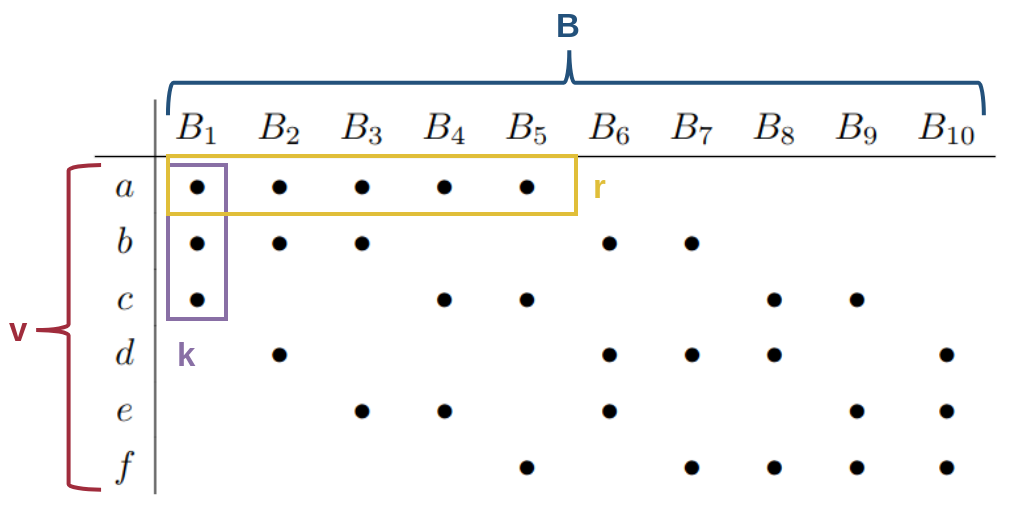
\includegraphics[width=\linewidth]{image/design.png}
\end{figure}
Daraus folgt $\mathbf{k \cdot b = r \cdot v}$. Somit muss $k$ ein Teiler von $rv$ sein. Da $8 \cdot 5 = 40$ nicht durch $3$ teilbar ist, kann es kein solches Design geben.  
\end{bsp} \noindent \rule{8cm}{0.4pt}
\explainvkrb
\begin{bsp} \label{bsp-5-4}
Gibt es ein Design mit Parametern $(8, 2, 9)$?  
Da alle $b$ Blöcke verschieden sein müssen, gilt $b \leq \binom{v}{k}$. Außerdem folgt aus $k \cdot b = r \cdot v$, dass $\frac{r \cdot v}{k} \leq \binom{v}{k}$.  
Für $(v, k, r) = (8, 2, 9)$ ist $\frac{r \cdot v}{k} = 36$, was größer ist als $\binom{8}{2} = 28$. Es kann also kein solches Design geben.  

Bemerkenswerterweise gibt es für jede Parameter, welche diese zwei Kriterien erfüllen, ein Design. 
\end{bsp} \noindent \rule{8cm}{0.4pt}\txc{\begin{anmerkung} \textbf{zum Vorgehen} 
\begin{enumerate}
    \item Ist $k$ Teiler von $rv$?
    \item Ist $b \leq \binom{v}{k}$? 
    \item Bzw. ist $\frac{v \cdot r}{k} \leq \binom{v}{k}$ ?
\end{enumerate}
\end{anmerkung}
}

\begin{satz}
Ein Design mit Parametern $(v, k, r)$ existiert genau dann, wenn $k \mid vr$ und $\frac{v \cdot r}{k} \leq \binom{v}{k}$.   \\
\txc{$\frac{v \cdot r}{k} \leq \binom{v}{k}$, denn
\[
k \cdot b = r \cdot v  \Rightarrow b = \frac{r \cdot v }{k}
\]
Also
\[
 b = \frac{r \cdot v }{k} \leq \binom{v}{k}
\]
Weil man die Anzahl der insgesamt möglichen Blöcke ($\binom{v}{k}$) nicht überschreiten darf!}
\paragraph{Beweis.}
Wir haben bereits in den Beispielen \ref{bsp-5-3} und \ref{bsp-5-4} gezeigt, dass jedes Design diese zwei Bedingungen erfüllt.  
Seien nun $(v, k, r)$ gegeben, welche die Bedingungen erfüllen, und sei $X$ eine $v$-elementige Menge.  
Setze $b = \frac{v \cdot r}{k}$.  

Wir wählen irgendeine Menge $\mathcal{C}$ von $b$ verschiedenen $k$-elementigen Teilmengen von $X$.  
Wir betrachten wie zuvor die Tabelle mit Zeilen, die Elemente von $X$, Spalten, die Elemente von $\mathcal{C}$,  
und Zelleneinträgen in $(x, C)$ gegeben durch Punkte, falls $x \in C$.  

Dann ist jede Spaltensumme gleich $k$, aber die Zeilensummen $r(x)$ hängen von $x$ ab. Zweifaches Abzählen \txc{(Siehe Seite \pageref{rsp:zweifach})} ergibt:
\txc{
\[
\sum_{x \in X} r(x) = bk.
\]
Da wir wissen, dass die beiden Arten die Elemente zu zählen das gleiche zählen. Setze $b = \frac{v \cdot r}{k}$:
\[
\sum_{x \in X} r(x) = \frac{v \cdot r}{k} \cdot k = vr
\]
Also: 
}
\[
\sum_{x \in X} r(x) = bk = vr.
\]
Sind alle $r(x)$ gleich, so ist $C$ schon ein Design\txc{, da $r = r(x)$ und somit die Bedingung erfüllt ist, dass jede Zeile $r$ Punkte hat - aka jedes Element $r$ mal vorkommt. (Die Bedingung, dass jede Spalte $k$ Elemente hat ist - aka jeder Block $k$ Elemente hat - ist bereits erfüllt, da wir explizit $k$-elementige Teilmengen als Blöcke gewählt haben.} \\ Andernfalls gibt es $x_1, x_2 \in X$ mit $r(x_1) > r > r(x_2)$.  
Sei $\mathcal{Q}_1$ die Menge der Blöcke $C \in \mathcal{C}$ mit $x_1 \in C$ aber $x_2 \notin C$.  
\explaindesign
Für $C \in \mathcal{Q}_1$ definieren wir:
\[
C^* := (C \setminus \{x_1\}) \cup \{x_2\},
\]
also wir ersetzen $x_1$ mit $x_2$. Wir schreiben $\mathcal{Q}_1^* := \{C^* \mid C \in \mathcal{Q}_1\}$ und bemerken, dass jedes $C^* \in \mathcal{Q}_1^*$  
$x_2$ enthält, aber nicht $x_1$.  

Sei $q$ die Anzahl von Blöcken, welche beide $x_1$ und $x_2$ enthalten. Dann gilt:
\[
|\mathcal{Q}_1| + q = r(x_1) > r(x_2),
\]
und daher auch:
\[ 
|\mathcal{Q}_1^*| + q > r(x_2).
\]
Das heißt, es gibt $C \in \mathcal{Q}_1$ mit $C^* \notin \mathcal{C}$.  

Sei $\mathcal{C}^*$ die neue Menge von Blöcken, erhalten durch Ersetzen von $C$ mit $C^*$.  
Die dazugehörigen Zeilensummen $r^*(x)$ sind gleich außer:
\[
r^*(x_1) = r(x_1) - 1 \quad \text{und} \quad r^*(x_2) = r(x_2) + 1.
\]
Die Zahl $\sum_{x \in X} |r(x) - r|$ hat sich also verringert.  
Nach endlich vielen Schritten ist diese Null und wir haben ein Design. \\ \newline
Die zweite Bedingung ist äquivalent zu 
\[
 r \leq \binom{v-1}{k-1}.
\] 
\txc{
Denn
\begin{align*}
    \frac{r \cdot v }{k} &  \leq \binom{v}{k} \\
   &  = \frac{v!}{k!(v-k)!} &  | \cdot k \\
    rv & \leq \frac{v!}{(k-1)!(v-k)!} & | \div v \\
    r & \leq \frac{(v-1)!}{(k-1)!(v-k)!} \\
    & = \frac{(v-1)!}{(k-1)!(v-k-1+1)!} \\
    & =  \frac{(v-1)!}{(k-1)!((v-1)- k +1)!} \\
   & =  \frac{(v-1)!}{(k-1)!((v-1)- (k -1))!} \\
   & = \binom{v-1}{k-1} 
\end{align*}
}
Die Notwendigkeit dieser Bedingung sehen wir auch folgendermaßen. Für jeden Block \( B \in \mathcal{B} \)
mit \( x_0 \in B \) ist \( B \setminus \{x_0\} \) eine \((k - 1)\)-elementige Teilmenge von \( X \setminus \{x_0\} \).
Da alle Blöcke, welche \( x_0 \) enthalten, verschieden sein müssen, kann es höchstens 
\[
\binom{v-1}{k-1}
\]
solche Blöcke geben.
\explainvkrb
Ersetzt man die Bedingung, dass alle Varietäten in gleich vielen Blöcken
vorkommen, durch die Bedingung, dass alle Paare von Varietäten in gleich
vielen Blöcken vorkommen, so spricht man von einem 2-Design. Allgemeiner siehe Definition \ref{defi5-6}.
 \end{satz} \noindent \rule{8cm}{0.4pt}

\txc{
\begin{anmerkung} \textbf{Übersetzt...} \\
Sind alle $r(x)$ gleich, so ist $\mathtt{D_i}$ schon ein Design. \\
Andernfalls gibt es $x_1, x_2 \in X$ mit $r(x_1) > r > r(x_2)$.  
Sei $\mathtt{M_{mitx1}}$ die Menge der Blöcke $\mathtt{D_i} \in \mathtt{D_{gesamt}}$ mit $x_1 \in \mathtt{D_i}$ aber $x_2 \notin \mathtt{D_i}$.   \\
Für $\mathtt{D_i} \in \mathtt{M_{mitx1}}$ definieren wir:
\[
\mathtt{D_i^{tausch}} := (\mathtt{D_i} \setminus \{x_1\}) \cup \{x_2\},
\]
also wir ersetzen $x_1$ mit $x_2$. \\ 
Wir schreiben $\mathtt{M_{mitx1}^{tausch}} := \{\mathtt{D_i^{tausch}} \mid \mathtt{D_i} \in \mathtt{M_{mitx1}}\}$ und bemerken, dass jedes $\mathtt{D_i^{tausch}} \in \mathtt{M_{mitx1}^{tausch}}$  
$x_2$ enthält, aber nicht $x_1$.  \\ 
Sei $q$ die Anzahl von Blöcken, welche beide $x_1$ und $x_2$ enthalten. Dann gilt:
\[
|\mathtt{M_{mitx1}}| + q = r(x_1) > r(x_2),
\]
weil man die Anzahl der Mengen in denen $x_1$, aber nicht $x_2$ vorkommt mit den Mengen addiert, in denen beide vorkommen. $x_1$ kommt öfter vor ($r(x_1)$) als $x_2$ vor kommt ($r(x_2)$), weil wir das zu Beginn so festgelegt haben. \\
Und daher auch:
\[ 
|\mathtt{M_{mitx1}^{tausch}}| + q > r(x_2).
\]
Denn
\[
|\mathtt{M_{mitx1}}| = |\mathtt{M_{mitx1}^{tausch}}| 
\]
Also
\[
|\mathtt{M_{mitx1}}| + q = |\mathtt{M_{mitx1}^{tausch}}| + q = r(x_1) > r(x_2).
\]
Das heißt, es gibt $\mathtt{D_i} \in \mathtt{M_{mitx1}}$ mit $\mathtt{D_i^{tausch}} \notin  \mathtt{D_{gesamt}}$, weil nach dem Tausch das neue $r(x_2)$ größer ist als das ursprüngliche und deshalb kann der Block mit Tausch ($\mathtt{D_i^{tausch}}$) nicht in der ursprünglichen Block-Menge ($\mathtt{D_{gesamt}}$) liegen, sondern muss in einer anderen/neuen Blockmenge ($\mathtt{D_{gesamt}^{tausch}}$) liegen. \\   
Sei $\mathtt{D_{gesamt}^{tausch}}$ diese neue Menge von Blöcken, erhalten durch Ersetzen von $\mathtt{D_i}$ mit $\mathtt{D_i^{tausch}}$.  \\
Die dazugehörigen Zeilensummen $\mathtt{r^{tausch}}(x)$ sind gleich außer:
\[
\mathtt{r^{tausch}}(x_1) = r(x_1) - 1 \quad \text{und } \mathtt{r^{tausch}}(x_2) = r(x_2) + 1.
\]
Die Gesamtabweichung der Zeilensummen vom Durchschnitt ($\sum_{x \in X} |r(x) - r|$) hat sich also um 2 verringert.  
Nach endlich vielen Schritten ist diese Null und wir haben ein Design.
\end{anmerkung}
}
\explaindesign
\explainrs

\begin{defi} \label{defi5-6}
Sei $X$ eine endliche Menge mit $|X| = v$. Eine Menge $\mathcal{B}$ von $k$-elementigen Teilmengen von $X$ heißt \textit{$t$-Design} mit Parametern $(v, k, r_t)$, wenn jede $t$-elementige Teilmenge von $X$ in genau $r_t$ Blöcken aus $\mathcal{B}$ enthalten ist.  

\noindent Ein 1-Design entspricht der ursprünglichen Definition eines Designs.  

\noindent \textit{Ist das Design von Problem \ref{prob5-1} ein 2-Design?}  
Nein, da $\{a, b\}$ in 3 Blöcken enthalten ist, aber $\{b, c\}$ nur in einem.
\end{defi} \noindent \rule{8cm}{0.4pt}

\begin{bsp}
Sei $v = 8$, $k = 4$, $r_3 = 1$ (somit $t = 3$) und $X = \{1, 2, \dots, 8\}$.  
Die Blöcke
\[
\{1, 2, 3, 5\}, \{1, 3, 4, 6\}, \{1, 4, 5, 7\}, \{1, 5, 6, 8\}, \{1, 2, 6, 7\}, 
\]
\[
\{1, 3, 7, 8\}, \{1, 2, 4, 8\}, \{4, 6, 7, 8\}, \{2, 5, 7, 8\}, \{2, 3, 6, 8\}, 
\]
\[
\{2, 3, 4, 7\}, \{3, 4, 5, 8\}, \{2, 4, 5, 6\}, \{3, 5, 6, 7\}
\]
bilden ein 3-Design.  

Die dazugehörige Tabelle ist:
\begin{table}[H]
\centering
\scalebox{0.7}{
\begin{tabular}{c|cccccccccccccc} 
    & $B_1$ & $B_2$ & $B_3$ & $B_4$ & $B_5$ & $B_6$ & $B_7$ & $B_8$ & $B_9$ & $B_{10}$ & $B_{11}$ & $B_{12}$ & $B_{13}$ & $B_{14}$ \\
\hline
1 & $\bullet$ & $\bullet$ & $\bullet$ & $\bullet$ & $\bullet$ & $\bullet$ & $\bullet$ & & & & & & & \\
2 & $\bullet$ & & & & $\bullet$ & & $\bullet$ & & $\bullet$ & $\bullet$ & $\bullet$ & & $\bullet$ & \\
3 & $\bullet$ & $\bullet$ & & & & $\bullet$ & & & & $\bullet$ & $\bullet$ & $\bullet$ & & $\bullet$ \\
4 & & $\bullet$ & $\bullet$ & & & & $\bullet$ & $\bullet$ &  & & $\bullet$ & $\bullet$ &$\bullet$ &  \\
5 & $\bullet$ & & $\bullet$ & $\bullet$ & & & & & $\bullet$ & & & $\bullet$ & $\bullet$ & $\bullet$\\
6 & & $\bullet$ & & $\bullet$ & $\bullet$ & & & $\bullet$ & & $\bullet$ & & & $\bullet$ & $\bullet$ \\
7 & & & $\bullet$ & & $\bullet$ & $\bullet$ & & $\bullet$ & $\bullet$ & & $\bullet$ & & & $\bullet$  \\
8 & & & & $\bullet$ &  & $\bullet$ & $\bullet$ & $\bullet$ & $\bullet$ & $\bullet$ & & $\bullet$ & & \\
\end{tabular}
}
\caption{Beispieltabelle}
\end{table}
\noindent Dies ist kein 4-Design, da $\{1, 2, 3, 5\}$ vorkommt, aber nicht $\{1, 2, 3, 6\}$.  
Jedoch ist es ein 2-Design und ein 1-Design. Dies ist kein Zufall gemäß dem folgenden Resultat.  
\end{bsp} \noindent \rule{8cm}{0.4pt}

\begin{bsp}
 Jedes $t$-Design ist auch ein $s$-Design für $1 \leq s \leq t$.  
\explainvkrb
\paragraph{Beweis.} Es genügt zu zeigen, dass für $t \geq 2$ ein $t$-Design auch ein $(t - 1)$-Design ist. Denn die Aussage folgt dann induktiv.  \\
Sei $\mathcal{B}$ ein $t$-Design von Teilmengen von $X$. Wir fixieren eine $(t - 1)$-elementige Teilmenge $S \subseteq X$.   \\
\txc{Bspw. $X=\{1,2,3,4,5\}$, $S=\{1,2\}$ und $\mathcal{B}=\{\{1,2,3\},\{1,2,4\},\{1,3,5\},\{2,4,5\},\{3,4,5\}\}$.} \\
Wir zählen die Paare $(x, B) \in X \times \mathcal{B}$, wobei $B$ ein Block ist, welcher $S$ enthält und $x \in B \setminus S$.  \\
\txc{Bspw. die Paare $(3,\{1,2,3\})$ und $(4,\{1,2,4\})$.} \\ 
Falls $B \in \mathcal{B}$ ein Block ist, welcher $S$ enthält, dann gibt es
\[
|B \setminus S| = |B| - |S| = k - (t - 1) = k - t + 1
\]
solche Elemente $x$.  \\
\txc{Bspw. $B = \{1,2,3\} \in \mathcal{B}$ mit
\[
|B \setminus S| = 3 - 2 = 3 - (3 - 1) = 3 - 3 + 1
\]}
Ist $r_S$ die Anzahl Blöcke, welche $S$ enthalten, dann ist die Anzahl der Paare $(x, B)$ gleich:
\[
r_S \cdot (k - t + 1).
\]
\txc{In unserem Beispiel
\[
2 \cdot (3 - 3 + 1) = 2.
\]}
Andererseits können wir die Paare auch zählen, indem wir für jedes $x \in X \setminus S$ \txc{($x \notin S$)} die Blöcke betrachten, welche $\{x\} \cup S$ enthalten. \txc{In unserem Beispiel wären diese $x$-e: $3,4,5$ und daher die möglichen Blöcke $\{x\} \cup S$: $\{1,2,3\}$, $\{1,2,4\}$ und $\{1,2,5\}$} \\
Da $|\{x\} \cup S| = t$ , gibt es $r_t$ viele solche Blöcke. Die Anzahl Paare $(x, B)$ ist somit:
\[
|X \setminus S| \cdot r_t = (v - (t - 1)) r_t = (v - t + 1) r_t.
\]
\txc{In unserem Beispiel:
\[
3 \cdot 1 = (5 - (3 - 1)) \cdot 1 = (5 - 3 + 1) \cdot 1 = 3.
\]}
Die zwei Berechnungen der Anzahl Paare liefern die Gleichung\txc{(weil zweimal das gleiche auf verschiedene Weisen gezählt wird)}:
\[
(v - t + 1) r_t = r_S \cdot (k - t + 1).
\]
Somit ist:
\[
r_S = r_t \cdot \frac{v - t + 1}{k - t + 1},
\]
unabhängig von der Wahl der $(t - 1)$-elementigen Teilmenge. Damit ist $\mathcal{B}$ ein $(t - 1)$-Design.  
\end{bsp} \noindent \rule{8cm}{0.4pt}
\explaindesign
\begin{folg} \explainvkrb \explainrs
Falls $\mathcal{B}$ ein $t$-Design ist mit Parametern $(v, k, r_t)$, dann ist $\mathcal{B}$ ein $s$-Design mit Parametern $v$, $k$ und
\[
r_s = r_t \cdot \frac{(v - s)(v - s - 1) \cdots (v - t + 1)}{(k - s)(k - s - 1) \cdots (k - t + 1)}
\]
für $1 \leq s < t$. Es gilt sogar auch für $s = 0$, wobei $r_0 = b$.  
\end{folg} \noindent \rule{8cm}{0.4pt}

\begin{folg}
Falls $\mathcal{B}$ ein $t$-Design mit Parametern $(v, k, r_t)$ ist, dann muss:
\[
(k - s)(k - s - 1) \cdots (k - t + 1)
\]
ein Teiler von
\[
r_t \cdot (v - s)(v - s - 1) \cdots (v - t + 1)
\]
sein für alle $0 \leq s < t$.  

Dies ist ein notwendiges Kriterium, das alle $t$-Designs erfüllen. Es gibt jedoch Mengen $\mathcal{B}$, welche diese Teilbarkeitskriterien erfüllen und trotzdem kein $t$-Design sind.  
\end{folg} \noindent \rule{8cm}{0.4pt}

\begin{bsp}
Sei $\mathcal{B}$ ein 2-Design mit Parametern $(v, k, r_2)$. Dann ist $\mathcal{B}$ insbesondere ein Design.  
Was ist die Replikationszahl $r$ vom Design $\mathcal{B}$?  
\[
r = r_1 = r_2 \cdot \frac{v - 1}{k - 1}.
\]
\end{bsp} \noindent \rule{8cm}{0.4pt}




\section{Partitionen}
\subsubsection*{Vorlesung 5 - 15.11.2024}
\addcontentsline{toc}{subsection}{Vorlesung 5}
\begin{defi}
Eine Partition (oder Klasseneinteilung) einer Menge \( X \) ist eine Menge \(\glspl{partition}\) von nichtleeren Teilmengen von \( X \), sodass jedes Element von \( X \) in genau einer der Mengen von \(\glspl{partition}\) liegt. \\
In Formeln:
\[
X = \bigcup_{A \in \glspl{partition}} A \quad \text{und} \quad A \cap B = \emptyset \text{ für } A, B \in \glspl{partition}, A \neq B.
\]
\end{defi} \noindent \rule{8cm}{0.4pt}
\begin{bsp}
Die Klasseneinteilung einer Schülerschaft entspricht einer Partition der Menge der Schüler und Schülerinnen.
\end{bsp} \noindent \rule{8cm}{0.4pt}

\begin{bem}
Ein Design mit Parametern \( (v, k, r) \) ist eine Partition genau dann, wenn die Replikationszahl \( r = 1 \) ist. Im Unterschied zu den Blöcken eines Designs, können die Teilmengen der Partition unterschiedliche Kardinalitäten haben.
\end{bem} \noindent \rule{8cm}{0.4pt}

\begin{satz}
Sei \( \glspl{S}(n, k) \) die Anzahl der Partitionen einer \( n \)-elementigen Menge in \( k \) Teile. Dann gilt:

\[
\glspl{S}(n, 1) = 1, \quad S(n, n) = 1, \quad \glspl{S}(n, k) = \glspl{S}(n - 1, k - 1) + k\glspl{S}(n - 1, k).
\]

Die Zahlen \( \glspl{S}(n, k) \) heißen Stirlingzahlen zweiter Art. Es gilt \( \glspl{S}(n, k) = 0 \) falls \( k = 0 \) oder \( k > n \). \\  

\paragraph{Beweis.}
Sei \( X \) eine \( n \)-elementige Menge.\txc{Bspw. $X = \{a,b,c,d\}$}. Falls eine Partition von \( X \) aus nur einer Teilmenge besteht, dann ist diese gerade \( X \). Somit ist \( \glspl{S}(n, 1) = 1 \)\txc{bzw. \( S(4, 1) = 1 \)}.

Jetzt fixieren wir \( z \in X \)\txc{bspw. $z = a$}. Wie viele Partitionen \(\glspl{partition}\) mit \( k \) Teilen gibt es, sodass \( \{z\} \in \glspl{partition} \)?\txc{Also bspw. wie viele \(\glspl{partition}\) mit \( k = 2 \) Teilen gibt es, sodass \( \{a\} \in \glspl{partition} \)? (Fall 1)} \\
So viele wie es Partitionen von \( X \setminus \{z\} \) \txc{($\{b,c,d\}$)}gibt mit \( k - 1 \)\txc{($1$)} Teilen, also \( \glspl{S}(n - 1, k - 1) \)\txc{bzw. \( S(3, 1) \)}.    

Wie viele Partitionen \( \glspl{partition} \) mit \( k \) Teilen gibt es, sodass \( \{z\} \notin \glspl{partition} \)?\txc{(Fall 2)} \\
So viele wie es Partitionen von \( X \setminus \{z\} \) in \( k \) Teile gibt, mal die Anzahl der Möglichkeiten, das Element \( z \) zu einer der Teilmengen hinzuzufügen, also \( k \cdot \glspl{S}(n - 1, k) \). 

Somit ist:
\[
S(n, k) = \underbrace{\glspl{S}(n - 1, k - 1)}_{\txc{Fall \ 1}} + \underbrace{k \cdot \glspl{S}(n - 1, k)}_{\txc{Fall \ 2}}.
\]
Beachte, dass \( \glspl{S}(n, k) = 0 \) für \( k > n \). Also ist:
\[
\glspl{S}(n, n) = \glspl{S}(n - 1, n - 1) + n \cdot \glspl{S}(n - 1, n) = \glspl{S}(n - 1, n - 1).
\]
\txc{Weil $n > n-1$ und somit $n \cdot S(n - 1, n) = n \cdot 0 = 0$.} \\ 
Da \( \glspl{S}(1, 1) = 1 \) gilt, ist \( \glspl{S}(n, n) = 1 \) durch Induktion. Die entsprechende Partition ist \( \glspl{partition} = \{\{x\} \mid x \in X\} \).
 \end{satz} \noindent \rule{8cm}{0.4pt}
Dank dieser Rekursionsformel können die Stirlingzahlen zweiter Art mit einer Pyramide ähnlich zum Pascalschen Dreieck berechnet werden.

\[
\begin{array}{ccccccc}
k& 1 & 2 & 3 & 4 & 5 \\
&1 & 1 \\
&1 & 1 & 1 \\
&1 & 3 & 1 \\
&1 & 7 & 6 & 1 \\
&1 & 15 & 25 & 10 & 1 \\
\end{array}
\]

Sei \( \glspl{partition} \) eine Partition von \( X \), und schreibe \( x \sim y \) falls \( x, y \in X \) in derselben Teilmenge aus \( \glspl{partition} \) liegen. Dann gilt für alle \( x, y, z \in X \):

\begin{enumerate}
    \item \( x \sim x \) (Reflexivität)
    \item \( x \sim y \Rightarrow y \sim x \) (Symmetrie)
    \item \( x \sim y \) und \( y \sim z \Rightarrow x \sim z \) (Transitivität)
\end{enumerate}

Eine Relation \( \sim \) mit diesen drei Eigenschaften heißt \textbf{Äquivalenzrelation}. \index{Äquivalenzrelation}

\begin{defi}
Eine Relation auf einer Menge \( X \) ist eine Teilmenge \( R \subseteq X \times X \). Wir schreiben \( x \sim y \), falls \( (x, y) \in R \).

Eine \textbf{Äquivalenzrelation} ist eine Relation, die reflexiv, symmetrisch und transitiv ist.
\end{defi} \noindent \rule{8cm}{0.4pt}

\begin{bsp}
 Auf \( X = \mathbb{Z} \) betrachten wir die folgenden Relationen:

\[
\begin{array}{|c|c|c|c|}
\hline
\text{Relation } x \sim y & \text{reflexiv} & \text{symmetrisch} & \text{transitiv} \\
\hline
x \leq y & \checkmark^{\txc{1}} & ^{\txc{2}}& \checkmark^{\txc{3}}   \\
2 \mid x - y & \checkmark^{\txc{4}} & \checkmark^{\txc{5}} & \checkmark^{\txc{6}} \\
|x - y| \geq 2 & ^{\txc{7}} & \checkmark^{\txc{8}} & ^{\txc{9}}  \\
|x| = |y| & \checkmark & \checkmark & \checkmark \\
\hline
\end{array}
\]
\color{Blue}
\textbf{$^{1}$} $x \leq y$ ist reflexiv, da  $x \leq x$ und $y \leq y$ immer wahr sind \\
\textbf{$^{2}$} bspw. gilt $2 \leq 3$, aber nicht $3 \leq 2$ \\
\textbf{$^{3}$} wenn $x \leq y$ und $y \leq z$, dann gilt immer $x \leq z$  \\
\textbf{$^{4}$} $2 \mid x - x$ bzw. $2 \mid y - y$ ist $2 \mid 0$ und das ist immer wahr \\
\textbf{$^{5}$} $y-x=-(x-y)$ und daher gilt sowohl $2 \mid x - y$, als auch $2 \mid y - x$ \\
\textbf{$^{6}$}  \\
\textbf{$^{7}$}  \\
\textbf{$^{8}$}  \\
\textbf{$^{9}$}  \\
\color{black}
Ist nun \( \sim \) irgendeine Äquivalenzrelation, dann definieren wir die Äquivalenzklasse von \( x \in X \) als

\[
[x] = \{ y \in X \mid x \sim y \}.
\]
\txc{Also ist $[x]$ die Menge aller Elemente in $X$, die mit $x$ in der gegebenen Äquivalenzrelation $\sim$ stehen.}\\ 
Beachte, dass \( [x] = [y] \) genau dann, wenn \( x \sim y \).
\end{bsp} \noindent \rule{8cm}{0.4pt}
\color{Blue}
\begin{info}
\color{Blue}
Als Klasse gilt in der Mathematik, Klassenlogik und Mengenlehre eine Zusammenfassung beliebiger Objekte, definiert durch eine logische Eigenschaft, die alle Objekte der Klasse erfüllen. Vom Klassenbegriff ist der Mengenbegriff zu unterscheiden. Nicht alle Klassen sind automatisch auch Mengen, weil Mengen zusätzliche Bedingungen erfüllen müssen. Mengen sind aber stets Klassen und werden daher auch in der Praxis in Klassenschreibweise notiert. 
\end{info}
\color{black}

\begin{bsp}
 Für \( X = \mathbb{Z} \) und die Äquivalenzrelation \( n \sim m \), falls \( n - m \) durch \( 2 \) teilbar ist, gibt es zwei Äquivalenzklassen:
\[
[0] = \{ \dots, -2, 0, 2, 4, \dots \}, \quad
[1] = \{ \dots, -3, -1, 1, 3, \dots \}.
\]
Bezüglich der Äquivalenzrelation \( x \sim y \), falls \( |x| = |y| \), sind die Äquivalenzklassen:
\[
[0] = \{0\}, \quad [1] = \{-1, 1\}, \quad [2] = \{-2, 2\}, \dots
\]
\end{bsp} \noindent \rule{8cm}{0.4pt}

\begin{satz}

Die Äquivalenzklassen bezüglich einer Äquivalenzrelation bilden eine Partition.

\paragraph{Beweis.} Wir zeigen, dass \(\glspl{partition} = \{[x] \mid x \in X\} \) eine Partition von \( X \) ist. Dass \( X = \bigcup_{x \in X} [x] \) gilt, ist klar. Falls \( [x] \cap [y] \neq \emptyset \), existiert \( z \in X \) mit \( x \sim z \) und \( y \sim z \). Dann \( x \sim y \), und \( [x] = [y] \)\txc{, weil Äquivalenzklassen sich niemals teilweise überschneiden, nur ganz oder gar nicht}.

Tatsächlich erhalten wir mittels dieser Zuordnungen eine Bijektion zwischen den Partitionen von \( X \) und den Äquivalenzrelationen auf \( X \).
 \end{satz} \noindent \rule{8cm}{0.4pt}

\begin{bsp}
 Sei \( X = \mathbb{Z} \times (\mathbb{Z} \setminus \{0\}) \) und \( (a, b) \sim (c, d) \), falls \( ad = bc \). Die Relation ist
\begin{itemize}
    \item \textbf{reflexiv}: \( ab = ba \), also \( (a, b) \sim (b, a) \),
    \item \textbf{symmetrisch}: \( ad = bc \implies cb = da \), also \( (a, b) \sim (c, d) \implies (c, d) \sim (a, b) \),
    \item \textbf{transitiv}: Angenommen, \( (a, b) \sim (c, d) \) und \( (c, d) \sim (e, f) \), also \( ad = bc \) und \( cf = de \). Dann folgt \( adf = bcf = bde \). Da \( d \neq 0 \) nach Voraussetzung, erhalten wir \( af = be \), also \( (a, b) \sim (e, f) \).
\end{itemize}

Die Äquivalenzklassen werden mit \( a/b \) bezeichnet und liefern die rationalen Zahlen.
\end{bsp} \noindent \rule{8cm}{0.4pt}

\begin{prob}
Wie viele Möglichkeiten gibt es, \( n \) Objekte in \( k \) Fächer zu verteilen, sodass kein Fach leer bleibt? Anders gesagt, wie viele surjektive Abbildungen \( X \to Y \) mit \( |X| = n \) und \( |Y| = k \) gibt es?
\end{prob}


\begin{satz}
Es gibt \gls{kSnk} surjektive Abbildungen \( X \to Y \), falls \( |X| = n \) und \( |Y| = k \).

\paragraph{Beweis.} Einer surjektiven Abbildung \(\glspl{partition} : X \to Y \) wird die Partition bestehend aus den \( k \) Urbildmengen
\[
p^{\glspl{urbild}}(\{y\}) = \{x \in X \mid p(x) = y\}
\]
zugeordnet. Für eine beliebige Partition von \( X \), gibt es \( k! \) Möglichkeiten, jedem Teil ein Element von \( Y \) zuzuordnen\txc{(Siehe Produktregel Seite \pageref{rsp:produktregel}).} Da eine surjektive Abbildung durch die entsprechende Partition zusammen mit diesen Zuordnungen bestimmt ist, gibt es \( k! S(n, k) \) surjektive Abbildungen. \txc{Anders: für jede der $S(n,k)$ möglichen Partitionen von $X$ gibt es $k!$ Möglichkeiten die Partitionen von $X$ Elementen aus $Y$ zuzuordnen.} 
 \end{satz} \noindent \rule{8cm}{0.4pt}

\begin{defi}

    Sei \( X \) eine \( n \)-elementige Menge und \( r_1, \dots, r_k \in \mathbb{N} \), sodass \( r_1 + \cdots + r_k = n \). Der Multinomialkoeffizient
\[
\glspl{multinomialkoeffizient}
\]
ist die Anzahl Abbildungen \( X \to \{1, 2, \dots, k\} \), sodass \( r_1 \) Elemente auf \( 1 \) abgebildet werden, \( r_2 \) Elemente auf \( 2 \), und so weiter.

Ist \( k = 2 \), dann gilt
\[
\binom{n}{r, n-r} = \binom{n}{r} = \binom{n}{n-r}.
\]
\end{defi} \noindent \rule{8cm}{0.4pt} \\
\txc{\noindent Verwendung: eine $n$-elementige Menge in $k$ Gruppen mit bestimmten Größen $r_1,r_2,…,r_k$ aufteilen, Anordnungen mit Wiederholungen, Teilbarkeitsbeweise}
\begin{satz}
Es gilt
\[
\binom{n}{r_1, r_2, \ldots, r_k} = \frac{n!}{r_1! r_2! \cdots r_k!}
\]
\paragraph{Beweis.} Eine Funktion \( X \rightarrow \{1, \ldots, k\} \) mit \( |X| = n \) sodass \( r_i \) Elemente auf \( i \) abgebildet werden, können wir dadurch beschreiben, dass wir zunächst \( r_1 \) Elemente auswählen, die auf \( 1 \) abgebildet werden. Dazu gibt es \( \binom{n}{r_1} \) Möglichkeiten. Danach wählen wir von den \( n - r_1 \) übrigen Elementen in \( X \), \( r_2 \) Elemente, welche auf \( 2 \) abgebildet werden. Dazu gibt es \( \binom{n - r_1}{r_2} \) Möglichkeiten. Wir machen so weiter und erhalten insgesamt
\[
\binom{n}{r_1} \cdot \binom{n - r_1}{r_2} \cdots \binom{n - (r_1 + \cdots + r_{k-1})}{r_k} = \frac{n!}{r_1! r_2! \cdots r_k!}
\]
Möglichkeiten.
 \end{satz} \noindent \rule{8cm}{0.4pt}
\begin{satz}
Es gilt
\[
(x_1 + x_2 + \cdots + x_k)^n = \sum_{r_1 + \cdots + r_k = n} \binom{n}{r_1, r_2, \ldots, r_k} x_1^{r_1} x_2^{r_2} \cdots x_k^{r_k}.
\]
\txc{Verwendung: zählen wie oft eine bestimmte Kombination vorkommt} 
\paragraph{Beweis.} Beim Ausmultiplizieren entsteht ein Term \( x_1^{r_1} x_2^{r_2} \cdots x_k^{r_k} \), wenn wir von \( r_1 \) Faktoren den Term \( x_1 \) wählen, von \( r_2 \) Faktoren den Term \( x_2 \) usw. Die Anzahl der Möglichkeiten, die Faktoren so auszuwählen, ist \( \binom{n}{r_1, r_2, \ldots, r_k} \).

 \end{satz} \noindent \rule{8cm}{0.4pt}
\begin{bsp}
Wie viele Anagramme kann man aus ABRACADABRA formen? Wir suchen die Anzahl der Funktionen \( \{x_1, \ldots, x_{11}\} \rightarrow \{A, B, C, D, R\} \), welche 5 Elemente auf \( A \) abbilden, 2 auf \( B \), 1 auf \( C \), 1 auf \( D \) und 2 auf \( R \). 

Also gibt es
\[
\binom{11}{5, 2, 1, 1, 2} = \frac{11!}{5!2!1!1!2!} = \frac{11 \cdot 10 \cdot 9 \cdot 8 \cdot 7 \cdot 6}{5 \cdot 2 \cdot 1 \cdot 1 \cdot 2} = 83160
\]
solcher Wörter.
\end{bsp} \noindent \rule{8cm}{0.4pt}

\section{Klassifikation von Permutationen (nf)}
\subsubsection*{Vorlesung 6 - 22.11.2024}
\addcontentsline{toc}{subsection}{Vorlesung 6}
Wie bereits erwähnt können wir die Elemente einer $n$-elementigen Menge $X$ durchnummerieren und daher alle Permutationen von $X$ durch Permutationen von $\{1, \dots, n\}$, also durch $\glspl{Sn}$, beschreiben. Konkret ist eine solche Durchnummerierung eine Bijektion $f: \{1, \dots, n\} \to X$. Jede Permutation $\alpha$ von $\{1, \dots, n\}$ liefert eine Permutation $\beta = f \alpha f^{\glspl{urbild}}$ von $X$ (und umgekehrt). \\
\txc{Beispielsweise $X=\{a,b,c\}$ mit $f(1)=a, f(2)=b, f(3)=c$ hat $f: \{1,2,3\} \rightarrow X$ und $f^{-1}:X \rightarrow\{1,2,3\}$, also $f^{-1}(a) =1, f^{-1}(b)=2, f^{-1}(c)=3$. \\ \newline
Anders: Um eine Permutation $\alpha$ auf einer nummerierten Menge (z.B. $\{1,2,…,n\}$) auf eine beliebige Menge $X$ zu übertragen, übersetze ich zuerst ein Element von $X$ zurück in seine Nummer mit $f^{-1}$, wende dort die Permutation $\alpha$ an, und übersetze das Ergebnis wieder in ein Element von $X$ mit $f$. Das ergibt die Permutation $\beta$ auf $X$, die die gleiche Struktur hat wie $\alpha$, nur auf anderen Namen
}

\begin{defi}
Zwei Permutationen $\alpha, \beta$ von $X$ heißen konjugiert, wenn es eine Permutation $\sigma$ von $X$ gibt, sodass $\beta = \sigma \alpha \sigma^{\glspl{urbild}}$.  
Dies liefert eine Äquivalenzrelation\txc{Also sind Konjugationen Äquivalenzrelation auf Permutationen}:
\begin{itemize}
    \item \textbf{Reflexivität:} $\alpha = \mathrm{id} \cdot \alpha \cdot \mathrm{id}^{\glspl{urbild}}$.
    \item \textbf{Symmetrie:} Ist $\beta = \sigma \alpha \sigma^{\glspl{urbild}}$, dann ist auch $\alpha = \sigma^{\glspl{urbild}} \beta (\sigma^{\glspl{urbild}})^{\glspl{urbild}}$.
    \item \textbf{Transitivität:} Aus $\beta = \sigma \alpha \sigma^{\glspl{urbild}}$ und $\gamma = \tau \beta \tau^{\glspl{urbild}}$ folgt $\gamma = (\tau \sigma) \alpha (\tau \sigma)^{\glspl{urbild}}$.
\end{itemize}
\end{defi} \noindent \rule{8cm}{0.4pt}

\begin{bem}
Konjugation mit einer Bijektion $f$ ist ein \gls{Homomorphismus}:   \index{Konjugation}
$f \cdot \mathrm{id} \cdot f^{\glspl{urbild}} = \mathrm{id}$ und $(f \alpha_1 f^{\glspl{urbild}})(f \alpha_2 f^{\glspl{urbild}}) = f (\alpha_1 \alpha_2) f^{\glspl{urbild}}$. \txc{Siehe Transivität}
\end{bem} \noindent \rule{8cm}{0.4pt}

\begin{bsp}
Die Zykel $\alpha = (2, 3, 6, 7)$ und $\beta = (1, 5, 3, 7)$ von $S_7$ sind konjugiert. Denn $\beta = f \alpha f^{\glspl{urbild}}$ gilt für die Bijektion $f$ gegeben durch:

\[
\begin{array}{c|ccccccc}
x & 1 & 2 & 3 & 4 & 5 & 6 & 7 \\
\hline
f(x) & 4 & 1 & 5 & 6 & 2 & 3 & 7
\end{array}
\]
\end{bsp} \noindent \rule{8cm}{0.4pt}

\begin{bem}
Jede konjugierte Permutation $\beta = f \alpha f^{\glspl{urbild}}$ eines Zykels $\alpha$ ist wieder ein Zyklus. Zum Beispiel, ist $\alpha = (x_1, x_2, \dots, x_l)$, so ist $f \alpha f^{\glspl{urbild}}$ der Zyklus $(f(x_1), f(x_2), \dots, f(x_l))$. \\
\txc{$\rightarrow$ Struktur wird erhalten!}
\end{bem} \noindent \rule{8cm}{0.4pt}

\begin{defi}
Eine Partition einer natürlichen Zahl $n$ ist eine \gls{multimenge} von positiven ganzen Zahlen $n_1, n_2, \dots, n_k$ mit $n_1 + n_2 + \cdots + n_k = n$. Sei $p_k(n) =$ Anzahl der Partitionen von $n$ in $k$ Teile, und  
\[
p(n) = \sum_{k=1}^n p_k(n) = \text{Anzahl aller Partitionen von } n.
\]
\end{defi} \noindent \rule{8cm}{0.4pt}

\begin{bsp}
Die Partitionen von $5$: \bluenote{\textit{\gls{multimenge}}: Wie eine normale Menge, aber Elemente dürfen mehrfach vorkommen}
\[
\begin{array}{ll}
\text{Schreibweise als Summe} & \text{Schreibweise als \gls{multimenge}} \\ \hline
5 & [5] \\
1+4 & [1 \cdot 4] \\
2+3 & [2 \cdot 3] \\
1+1+3 & [1^2 \cdot 3] \\
1+2+2 & [1 \cdot 2^2] \\
1+1+1+2 & [1^3 \cdot 2] \\
1+1+1+1+1 & [1^5]
\end{array}
\]
\end{bsp} \noindent \rule{8cm}{0.4pt}

\begin{defi} \index{Typ einer Permutation}
Der Typ einer Permutation $\pi \in \glspl{Sn}$ ist die Partition von $n$, welche durch die Länge der disjunkten Zykel von $\pi$ gegeben ist.
\end{defi} \noindent \rule{8cm}{0.4pt}

\begin{bsp}
Der Typ von $\pi = (1, 3, 7)(2, 6)(4, 5, 8)(9)$ in $S_9$ ist $[1 \cdot 2 \cdot 3^2]$.
\end{bsp} \noindent \rule{8cm}{0.4pt}

\begin{satz}
Zwei Permutationen $\alpha, \beta \in \glspl{Sn}$ sind genau dann konjugiert, wenn sie denselben Typ haben.

\paragraph{Beweis.}\texttt{TODO} Ist $\beta = f \alpha f^{\glspl{urbild}}$ und $\alpha = \alpha_1 \cdots \alpha_k$ die Zerlegung in disjunkte Zykel, dann sind $\beta_i = f \alpha_i f^{\glspl{urbild}}$ disjunkte Zykel derselben Länge wie $\alpha_i$ für alle $1 \leq i \leq k$ und es gilt $\beta = \beta_1 \cdots \beta_k$. Also haben $\alpha$ und $\beta$ denselben Typ.  

Umgekehrt, nehmen wir an, dass $\alpha$ und $\beta$ denselben Typ haben. Seien $\alpha_1, \dots, \alpha_k$ die disjunkten Zykel von $\alpha$ und $\beta_1, \dots, \beta_k$ die disjunkten Zykel von $\beta$, jeweils in aufsteigender Zykellänge geordnet. Wir definieren eine Bijektion $f$ wie folgt:  
Für jedes Paar von Zykeln $\alpha_i$ und $\beta_i$, schreiben wir $\alpha_i = (x_1, \dots, x_l)$ und $\beta_i = (y_1, \dots, y_l)$, und setzen $f(x_j) := y_j$. Da jeder $x \in \{1, \dots, n\}$ in genau einen Zyklus $\alpha_i$ vorkommt, ist $f$ eine Bijektion. Dann gilt $\beta_i = f \alpha_i f^{\glspl{urbild}}$ für alle $i$, und dadurch auch $\beta = f \alpha f^{\glspl{urbild}}$. Also sind $\alpha$ und $\beta$ konjugiert.
 \end{satz} \noindent \rule{8cm}{0.4pt}

\begin{satz}
Für die Anzahl Permutationen $\glspl{snk}(n, k)$ in $\glspl{Sn}$ \txc{(eine $n$-elementige Menge)} mit $k$ disjunkten Zykeln gilt:
\[
\glspl{snk}(n, k) = \sum_{(\alpha_1, \dots, \alpha_n)} \frac{n!}{1^{\alpha_1} 2^{\alpha_2} \cdots n^{\alpha_n} \cdot \alpha_1! \alpha_2! \cdots \alpha_n!},
\]
wobei über alle $(\alpha_1, \dots, \alpha_n)$ summiert wird mit $\alpha_i \geq 0$, $\alpha_1 + \cdots + \alpha_n = k$ und $1 \cdot \alpha_1 + 2 \cdot \alpha_2 + \cdots + n \cdot \alpha_n = n$.

Die Zahlen $\glspl{snk}(n, k)$ heißen Stirlingzahlen erster Art. Es gilt:
\[
\sum_{k=1}^n \glspl{snk}(n, k) = n!, \quad \glspl{snk}(n, 1) = (n-1)!, \quad \glspl{snk}(n, n) = 1.
\]
\txc{
Denn:
\begin{align*}
    \sum_{k=1}^n \glspl{snk}(n, k) & = \glspl{snk}(n,1) + \sum_{k=2}^n \glspl{snk}(n, k) \\
    & =  (n - 1)! + \sum_{k=2}^n \glspl{snk}(n, k) \\
    & =  (n - 1)! + \glspl{snk}(n, 2) + \sum_{k=3}^n \glspl{snk}(n, k) \\
    & =  (n - 1)! + \big( n \cdot \glspl{snk}(n-1, 2) + \glspl{snk}(n-1, 1) \big) + \sum_{k=3}^n \glspl{snk}(n, k) \\
     & =  (n - 1)! + \big( n \cdot ( (n-1) \cdot \glspl{snk}(n-2, 2) + (n-3)!) + (n-2)! \big) + \sum_{k=3}^n \glspl{snk}(n, k) \\
     & = (n - 1)! + \big( n \cdot ( (n-1) \cdot ( + \cdots +( 3 \cdot  \glspl{snk}(2, 2) + 1! ) \cdots ) (n-3)!) + (n-2)! \big) + \sum_{k=3}^n \glspl{snk}(n, k) \\
      & = (n - 1)! + \big( n \cdot ( (n-1) \cdot ( \cdots ( 3 \cdot  1 + 1 ) + \cdots ) + (n-3)!) + (n-2)! \big) + \sum_{k=3}^n \glspl{snk}(n, k) \\
    & = (n - 1)! + \big( n \cdot ( (n-1) \cdot ( \cdots ( 4 ) + \cdots) +(n-3)!) + (n-2)! \big) + \sum_{k=3}^n \glspl{snk}(n, k) \\
\end{align*}
}
 \end{satz} \noindent \rule{8cm}{0.4pt}

\begin{bsp}
Sei $n = 5$:
\begin{table}[h!]
\centering
\begin{tabular}{|l|l|l|l|}
\hline
\textbf{Typ} & \textbf{Beispiel} & \textbf{k} & \textbf{Anzahl} \\
\hline
$[1^5]$ & $\mathrm{id}$ & 5 & 1 \\
$[1^3 \cdot 2]$ & $(1)(2)(3)(4,5)$ & 4 & 10 \\
$[1^2 \cdot 3]$ & $(1)(2)(3,4,5)$ & 3 & 20 \\
$[1 \cdot 2^2]$ & $(1)(2,3)(4,5)$ & 3 & 15 \\
$[1 \cdot 4]$ & $(1)(2,3,4,5)$ & 2 & 30 \\
$[2 \cdot 3]$ & $(1,2)(3,4,5)$ & 2 & 20 \\
$[5]$ & $(1,2,3,4,5)$ & 1 & 24 \\
\hline
\end{tabular}
\end{table}
\end{bsp} \noindent \rule{8cm}{0.4pt}

\begin{satz}
Für $n, k > 0$ gilt:
\[
\glspl{snk}(n, k) = s(n-1, k-1) + (n-1)\glspl{snk}(n-1, k).
\]
\paragraph{Beweis.} Siehe Aufgabenblatt 7.  
Wir erhalten das folgende Dreieck der Stirlingzahlen erster Art $\glspl{snk}(n, k)$:

\[
\begin{array}{c|cccccc}
n & k=1 & k=2 & k=3 & k=4 & k=5 & k=6 \\
\hline
1 & 1 \\
2 & 1 & 1 \\
3 & 2 & 3 & 1 \\
4 & 6 & 11 & 6 & 1 \\
5 & 24 & 50 & 35 & 10 & 1 \\
\end{array}
\] 

Es gibt eine statistische Methode der Populationsgenetik, bei der Stirlingzahlen erster Art berechnet werden müssen. Die Zahlen $\glspl{snk}(n, k)$ wachsen schnell. Für festes $k$ und $n \to \infty$ gibt es eine asymptotische Berechnung.  

Es wird weiterhin an asymptotischen Berechnungen von Ausdrücken geforscht, die Stirlingzahlen beinhalten. Siehe zum Beispiel:  
\url{https://www.g3journal.org/content/10/11/3959}

 \end{satz} \noindent \rule{8cm}{0.4pt}



\section{Teilbarkeit und Zahlenkongruenz (nf)}
\subsubsection*{Vorlesung 7 - 29.11.2024}
\addcontentsline{toc}{subsection}{Vorlesung 7}
$m \in \mathbb{Z}$ ist ein Teiler von $n\in \mathbb{Z}$, falls es ein $k \in \mathbb{Z}$ gibt mir $n = k \cdot m$. \\
Notation: $m \mid n$

\begin{er}
$a,b,d,x,y \in \mathbb{Z}$
\begin{enumerate}
    \item $x \neq 0$ und $d \mid x \Rightarrow \frac{x}{d} \mid x$
    \item $x \mid y$ und $y \mid z \Rightarrow x \mid z$
    \item $d \mid x$ und $d \mid y \Rightarrow d \mid ax + by$ \bluenote{3: Abgeschlossenheit unter linearer Kombination}
\end{enumerate}
Insbesondere sind die gemeinsamen Teiler von $x$ und $y$ dieselben wie die
gemeinsamen Teiler von $x - y$ und $y$. Dies führt zum euklidischen Algorithmus:
\end{er} \noindent \rule{8cm}{0.4pt}

\begin{bsp}
(Berechnung von \gls{ggt}(708, 222)) \texttt{TODO}
\end{bsp} \noindent \rule{8cm}{0.4pt}

% Satz 8.3
\begin{satz} \label{satz8-2} \txc{\textbf{Satz von Bézout} }\\
Für alle $x,y \in \mathbb{Z}$ gibt es $a,b \in \mathbb{Z}$ sodass $\gls{ggt}(x,y) = ax + by$.
 \end{satz} \noindent \rule{8cm}{0.4pt}
\begin{folg}
Wenn $d\mid x$ und $d\mid y$, dann $d\mid \gls{ggt}(x,y)$. \\
\txc{Wenn $d$ sowohl $x$ als auch $y$ teilt, ist es auch ein Teiler des Produktes von $x$ und $y$.}
\end{folg} \noindent \rule{8cm}{0.4pt}
\begin{folg}
Wenn $d\mid xy$ und $\gls{ggt}(x,d) = 1$, dann $d\mid y$. \\
\txc{Wenn $d$ ein Teiler von dem Produkt aus $x$ und $y$ ist, aber $d$ kein Teiler von $x$ ist, muss $d$ ein Teiler von $y$ sein.}
\paragraph{Beweis.} 
$1 = ax + bd$ und $kd = xy$ für $a,b,k \in \mathbb{Z}$ \\
$y=y \cdot 1 = y(ax +bd) = akd +bd = (ak +b)d \Rightarrow d\mid y$
\end{folg} \noindent \rule{8cm}{0.4pt}
\begin{folg}
Jede ganze Zahl hat eine eindeutige Primfaktorzerlegung. 
\end{folg} \noindent \rule{8cm}{0.4pt}


\begin{defi}
Seien $m,n,d \in \mathbb{Z}$ und $m \geq l$. Wir schreiben $m \equiv n \mod d$ \txc{(sprich: m kongruent zu n modulo d)}, falls $d \mid (m-n)$, d.h. $m$ und $n$ haben denselben Rest bei Division durch $d$ \txc{(modulo d)}. \\
Kongruenz modulo $d$ ist eine Äquivalenzrelation auf $\mathbb{Z}$.
Die \underline{Restklasse} von $m$ modulo $d$ wird mit $[m]_d$ bezeichnet und ist die Äquivalenzklasse von $m \in \mathbb{Z}$.  \\
$\mathbb{Z} / d\mathbb{Z} = \{[m]_d \mid m \in \mathbb{Z}\}$ \\
Es gibt genau $d$ Restklassen\txc{, denn wir Zählen immer $0$ bis $d-1$ und dass ist $s$}. 
\end{defi} \noindent \rule{8cm}{0.4pt} \index{Restklasse}
\begin{bsp}
 Um wie viele Wochentage verschiebt sich ein Datum pro Jahr? \\
 \txc{Relevant dabei sind die zwei folgenden Zahlen:}
 \begin{itemize}
     \item 365 Tage pro Jahr 
     \item 7 Tage pro Woche 
 \end{itemize}
 $\Rightarrow$ $365 \equiv 15 \equiv 1 \mod 7$\\
 d.h. der 29.11.2024 ist ein Freitag und der 29.11.2024 ist ein Samstag\txc{, da sich der Wochentag um einen Tag verschiebt}. 
\end{bsp} \noindent \rule{8cm}{0.4pt}
\begin{satz} \label{satz-8-9}
Seien $a \equiv x \mod m$\\
$b \equiv y \mod m$ \\
Dann gilt: $a+b \equiv x+y \mod m$ und $ab \equiv xy \mod m$\\
\textbf{Beweis}: 
\begin{align*}
   &  m \mid  (a-x) \text{ und } m \mid (b-y) \\
    \Rightarrow &  m \mid (a-x+b-y) = (a+b-(x-y)) \\
    & m \mid (a(b-y)+y(a-x)) = (ab-xy)
\end{align*}
 \end{satz} \noindent \rule{8cm}{0.4pt}
\begin{bsp}
Ist 31785 durch 9 teilbar? \\
\txc{Solche Fragen kann man generell mit der Quersumme herausfinden.}\\
$3+1+7+8+5=24$ ist nicht durch 9 teilbar, also ist  31785 nicht durch 9 teilbar. \\
\textbf{Beweis}: Sei $x = x_0 + x_1 \cdot 10 + x2 \cdot 10^2 + \cdots + x_n \cdot 10^n$, wobei $x_0, ..., x_n \in \{0,...,9\}$ \\
$x = x_0 + x_1 \cdot 10 + x2 \cdot 10^2 + \cdots + x_n \cdot 10^n \equiv x_0 + x_1 + x_2 + \cdots + x_n \mod 9$, da $10^i \equiv 1 \mod 9$
\end{bsp} \noindent \rule{8cm}{0.4pt} \\
Aufgrund von Satz \ref{satz8-2} können wir Addition und Multiplikation auf Restklassen definieren: 
\begin{defi}
$x,y,m \in \mathbb{Z}, m\geq 1$ (geht wegen Satz \ref{satz-8-9}) \\
$[x]_m + [y]_m := [x+y]_m$ und $[x]_m \cdot [y]_m := [xy]_m$
\end{defi} \noindent \rule{8cm}{0.4pt}
\begin{bsp}
$m = 2, \quad [0]_m + [1]_m = [1]_m$ d.h. die Summe einer geraden und ungeraden Zahl ist immer ungerade. 
\end{bsp} \noindent \rule{8cm}{0.4pt}
\begin{satz}
Die Restklassen modulo $m$ bilden einen \underline{kommutativen Ring} mit Einselement $[1]_m$. \\
Das bedeutet \txc{sozusagen, dass auch die restlichen Rechenregeln gelten}:
\begin{enumerate}
    \item $+$ und $\cdot$ sind assoziativ \bluenote{\textit{assoziativ}: Klammern setzen Ding: $[x]_m + [y]_m + [z]_z = [x]_m + ([y]_m + [z]_z)$; gilt eigentlich immer} und kommutativ \bluenote{\textit{kommutativ}: Das vertauschen: $[x]_m + [y]_m = [y]_m + [x]_m$; gilt nicht überall, z.B. nicht bei der Multiplikation von Matrizen)}
    \item das Distributivgesetz gilt \bluenote{\textit{distributiv}: Man kann ausklammern} 
    \item Existenz der Identität: \[ [x]_m + [0]_m = [x]_m \text{ und } [x]_m \cdot [1]_m = [x]_m\]
    \item Existenz der additiven Inversen 
    \[ [x]_m + [-x]_m = [0]_m \]
\end{enumerate}
 \end{satz} \noindent \rule{8cm}{0.4pt} \\
Was in der Liste "fehlt": Das Multiplikative Inverse. 
\begin{bsp}
$\mathbb{Z}/6\mathbb{Z}$ \\
\begin{tabular}{c|cccccc}
    $\cdot$ & $[0]_6$ & $[1]_6$ & $[2]_6$ & $[3]_6$ & $[4]_6$ & $[5]_6$   \\ \hline
    $[0]$ & $[0]$ & $[0]$ & $[0]$ & $[0]$ & $[0]$ & $[0]$ \\
    $[1]$ & $[0]$ & $[1]$ & $[2]$ & $[3]$ & $[4]$& $[5]$ \\
    $[2]$ & $[0]$ & $[2]$ & $[4]$ & $[0] = [6]$ & $[2]$ & $[4]$ \\
    $[3]$& $[0]$& $[3]$& $[0]$& $[3]$& $[0]$& $[3]$\\
    $[4]$ & $[0]$& $[4]$& $[2]$& $[0]$&$[4]$ &$[2]$ \\
    $[5]$ &$[0]$ &$[5]$ &$[4]$ &$[3]$ &$[2]$ & $[1] = [25]$\\
\end{tabular} \\  \newline
\txc{Alle Zahlen die einen größten gemeinsamen Teiler größer als 1 mit 6 haben sind die, die kein Inverses haben. \\ Hier haben nur $[1]$ und $[5]$ ein Inverses, weil sie teilerfremd zu $6$ sind: $\gls{ggt}(1,6) = 1 = \gls{ggt}(5,6)$ und bei den anderen Zahlen ist es $\gls{ggt}(2,6) =   2 = \gls{ggt}(4,6)$ bzw. $\gls{ggt}(3,6) = 3$.} \\
Ein Element $[x]_m$ heißt \underline{invertierbar}, falls es ein $[y]_m$ gibt mit \[[x]_m \cdot [y]_m = [1]_m\]
Wir sagen $[y]_m$ ist das Inverse von $[x]_m$.
\end{bsp} \noindent \rule{8cm}{0.4pt}
\begin{satz}
EIn Element $[x]_m$ in $\mathbb{Z} / m \mathbb{Z}$ ist invertierbar genau dann, wenn $\gls{ggt}(x,m) = 1$. \\
\textbf{Beweis}: $(\Rightarrow)$ $[x]_m \cdot [y]_m = [1]_m$, d.h. $xy \equiv 1 \mod m$ \\
$\Rightarrow xy + am = 1 \Rightarrow \gls{ggt}(x,m) \mid 1 \Rightarrow \gls{ggt}(x,m) = 1$\\
$(\Leftarrow)$ Sei $\gls{ggt}(x,m) = 1$. Dann erhalten wir durch Satz \ref{satz8-2}
\[ 1 = ax + bm\]
\[ [1]_m = [ax+bm]_m = [ax]_m = [a]_m [x]_m\]
 \end{satz} \noindent \rule{8cm}{0.4pt}
\begin{folg}
Die Menge der invertierbaren Elemente ist $(\mathbb{Z} / m \mathbb{Z})^{\times} = \{[x]_m \mid \gls{ggt}(x,m) = 1\}$. \\
$\phi(m) := \mid (\mathbb{Z} / m \mathbb{Z})^{\times} \mid $ heißt \underline{Eulersche phi Funktion} \txc{und zählt die Anzahl der invertierbaren Elemente in $\mathbb{Z} / m \mathbb{Z}$, also wie viele Zahlen von 1 bis $m-1$ teilerfremd zu $m$ sind }.
\end{folg} \noindent \rule{8cm}{0.4pt} 
\begin{bsp}
\bluenote{ $\phi(6)$: Wie viele Restklassen von 6 sind invertierbar?}
$\phi(6) = 2$\\
Weiter: \\
$\phi(2) = 1$ \\
$\phi(3) = 2$ \\
Für $p \ prim$ \bluenote{$p$: eine beliebige Primzahl} gilt: $\phi(p) = p-1$.\\
In $\mathbb{Z} / p \mathbb{Z}$ ist jedes Element außer $[0]_p$ invertierbar. Das bedeutet, dass $\mathbb{Z} / p \mathbb{Z}$ ein \Gls{Körper} ist. Häufig schreibt man $\mathbb{F}_p = \mathbb{Z} / p \mathbb{Z}$. 
\bluenote{$\mathbb{F}$, weil \Gls{Körper} im englischen Field heißen.}
\end{bsp} \noindent \rule{8cm}{0.4pt}
\begin{satz} (Euler) \texttt{TODO} \\ \bluenote{Verwendung: Modular Inverses berechnen, Vereinfachung großer Potenzen mod m}
Falls $\gls{ggt}(x,m) = 1$, so gilt $x^{\phi (m)} \equiv 1 \mod m$.\\
\paragraph{Beweis.} 
Seien $y_1, ..., y_{\phi(m)}$ alle Elemente in $(\mathbb{Z} / m \mathbb{Z})^{\times}$. Setze $y := y_1, ..., y_{\phi(m)}$
\begin{align*}
    (\mathbb{Z} / m \mathbb{Z})^x & langerpfeil (\mathbb{Z} / m \mathbb{Z})^x  \text{ ist eine Bijektion}\\
    a & langerPfeilmitstrichrichtunga a \cdot [x]_m
\end{align*}
Somit gilt $ y = (y_1 [x]_m) ... (y_{\phi(m)}[x]_m) = y [x]_m^{\phi(m)}$ \\
$\Rightarrow [1]_m = [x]_m^{\phi(m)} \Rightarrow x^{\phi(m)} \equiv 1 mod m$
 \end{satz} \noindent \rule{8cm}{0.4pt}
\begin{folg}
(Kleiner Satz von Fermat) \\
Ist $p$ eine Primzahl und $x$ eine ganze Zahl, so gilt
\[x^p \equiv x \mod p\]
\end{folg} \noindent \rule{8cm}{0.4pt}
\begin{bsp} \texttt{TODO}
\txc{Anwendung von }\\
Was ist die letzte Ziffer von $7^{358}$? \\
\txc{Wenn uns die letzte Ziffer interessiert, brauchen wir 10}\\
$\gls{ggt}(7,10) = 1, \phi(10) = \mid \{1,3,7,9\} = 4$ \\
$7^{358} = 7^{4 \cdot 89 +2} \equiv  7^{4^{89}} \cdot 7^{2} \equiv 1^{89} \cdot 7^{2} \equiv 49 \equiv  9 \mod 10$.
\end{bsp} \noindent \rule{8cm}{0.4pt}
\section{Zyklische Konstruktion von Designs (nf)}
\subsubsection*{Vorlesung 8 - 06.12.2024}
\addcontentsline{toc}{subsection}{Vorlesung 8}
\textbf{Kurze Wdh.:} $m \geq 1$ für $\mathbb{Z} / m \mathbb{Z} = \{[0]_m, [1]_, ..., [m-1]_m\}$ \\
Notation, wenn klar ist, dass es um Restklassen geht: $[i]_m = [i] = \bar{i} = i$ \\
Reminder: Es geht, um Ringe also haben wir $\cdot$ und $+$ \\
$(\mathbb{Z} / m \mathbb{Z})^{\times} = $ Menge der (mult.) invertierbaren Elemente in $\mathbb{Z} / m \mathbb{Z}$

Ein \underline{Design} von einer $v$-elementigen Menge $X$ mit Parametern $(v,k,r)$ ist eine Menge $\mathcal{B}$ von $k$-elementigen Teilmengen von $X$ sodss jedes $x ¸\in X$ in genau $r$ Blöcke von $\mathcal{B}$ vorkommt. \\
\underline{Idee}: $X = \mathbb{Z} / m \mathbb{Z}$, $S \subseteq \mathbb{Z} / m \mathbb{Z}$, $S+i = \{ a+i \mid i \in S\}$ \\
 \noindent \rule{8cm}{0.4pt} 
\begin{bsp}
$ m = 4, X = \mathbb{Z} / m \mathbb{Z}, S = \{0,1\}$ 
\begin{table}[H]
    \centering
    \begin{tabular}{c|cccc}
         &  $S+0 = \{0,1\}$  & $S+1 = \{1,2\}$ & $S+2$ & $S+3$  \\
         0 & * & &  & * \\
         1 & * & * & & \\
         2 & & * & * & \\
         3 & & &  * & * \\
    \end{tabular}
\end{table} \bluenote{(4,2,2): 4 Elemente, 2 Elemente pro Block, jedes Element kommt in 2 Blöcken vor}
\noindent Das ist ein Design mit Parametern $(4,2,2)$. \\ \newline
Weiteres Beispiel: $ M = 4, S = \{0,2\}$
\begin{table}[H]
    \centering
    \begin{tabular}{c|cc}
         &  $S+0 = S+2$ & $S+1 = S+3$  \\
         0 & * &   \\
         1 & & *  \\
         2 &  * & \\
         3 & & *  \\
    \end{tabular}
\end{table}
\bluenote{\textbf{Reminder}: \(\{0,2\} = \{2,0\}\)}
\noindent Das ist ein Design mit Parametern $(4,2,1)$. \txc{Das ist immer noch ein Design! Man schreibt aber $S+2$ und $S+3$ nicht explizit hin, weil Blöcke nicht doppelt vorkommen sollen.}
\end{bsp} \noindent \rule{8cm}{0.4pt}

\begin{beo}
Diese Konstruktion liefert immer ein Design! Denn $a$ kommt im Block
$S + i$ vor genau dann wenn $0$ im Block $S + i - a$ vorkommt. \bluenote{$a \in S+i \Leftrightarrow 0 \in S+(i-1)$} \\ 
Anzahl an Blöcken: $ b = \frac{m}{z}$
$v = m, k = \mid S \mid, r = \frac{kb}{v}= \frac{k}{z}, z =\mid \{ i \in \mathbb{Z} / m \mathbb{Z} \mid S = S+i \} \mid $ \\

\end{beo} \noindent \rule{8cm}{0.4pt}

\begin{fr}
Sind diese Designs immer 2-Designs? Wann erhalten wir durch diese Konstruktion 2-Designs? \\
\txc{Was macht nochmal ein 2-Design aus? Raus suchen} \\
d.h. für jede 2-elementige Teilmenge $\{a,b\}, a \neq b$ gibt es genau $r_2$ Blöcke, die $a,b$ enthalten. \\ \txc{Ist das bei unserem Bsp. der Fall ? 
\begin{table}[H]
    \centering \color{Blue}
    \begin{tabular}{c|cccc}
         &  $S+0$ & $S+1$ & $S+2$ & $S+3$  \\
         $\{a,b\}$ & $\{0,1\}$ & $\{1,2\}$ & $\{2,3\}$ & $\{0,3\}$ \\ \hline
         0 & * & &  & * \\
         1 & * & * & & \\
         2 & & * & * & \\
         3 & & &  * & * \\
    \end{tabular}
\end{table}
\noindent Reminder: Jede der $\binom{v}{t} = \binom{4}{2}$ Teilmengen von $X$ muss $r_2$-mal in dem Design vorkommen. \\  
$\{0,1\}$ ist in einem Block \\
$\{0,2\}$ ist in keinem Block ! \\
$\{0,3\}$ ist in einem Block \\
Hier ist das Problem wir haben keine Differenz, die 2 ist, weil die Zahlen 0 und 1 ja aufeinander Folgen und da nie die Differenz 2 existieren kann. \\ Differenzen meint hier: Man kann Paare wie $\{a,b\}$ auch durch ihre Differenz charakterisieren. Alle Blöcke enthalten Paare mit Differenz 1 modulo 4.  \\
Es ist also kein 2-Design weil manche Differenzen (hier: 2) nicht vorkommen. \\
$\Rightarrow$ kein 2-Design! \\
Und unser anderes Beispiel? 
\begin{table}[H]
    \centering \color{Blue}
    \begin{tabular}{c|cc}
         &  $S+0 = S+2$ & $S+1 = S+3$  \\
         0 & * &   \\
         1 & & *  \\
         2 &  * & \\
         3 & & *  \\
    \end{tabular}
\end{table}
\noindent $\{0,1\}$ ist in keinem Block enthalten! \\
$\{0,2\}$ ist in einem Block enthalten\\
$\Rightarrow$ kein 2-Design 
}
\end{fr} \noindent \rule{8cm}{0.4pt}

\begin{bsp}
$m = 5$, $S = \{0,1,2\}$ \\
\bluenote{Hier sind jetzt Differenzen von 2 möglich! (z.B. $0-2$)}
\begin{table}[H]
    \centering
    \begin{tabular}{c|ccccc}
         &  $S+0$ & $S+1$ & $S+2$ & $S+3$ & $S+4$  \\ \hline
         0 &*& & &*&*\\
         1 &*&*& & &*\\
         2 &*&*&*& & \\
         3 & &*&*&*& \\
         4 & & &*&*&*\\
    \end{tabular}
\end{table}
\noindent Ist das ein 2-Design? \\
$\{0,1\}$ kommt zwei mal vor. $\{1,3\}$ und $\{0,2\}$ aber nur ein mal. Wieder kein 2-Design. \\
\bluenote{Hier kommen zwar alle Differenzen vor, aber es kommen nicht alle zweier-Kombis gleich oft vor bzw. nicht alle Differenzen gleich oft vor.}
\end{bsp} \noindent \rule{8cm}{0.4pt} \\
\txc{\noindent Explizit gemacht was bedeutet, dass alle Differenzen (nicht) gleich oft vorkommen:}
\begin{defi}
Eine Menge $S \subseteq \zat$ heißt \underline{Differenzenfamilie}, wenn unter den Differenzen $x-y, \quad x,y \in S, \quad x \neq x$ jedes Element von $\zat \backslash \{0\}$ gleich oft vorkommt. \index{Differenzenfamilie} \\ 
d.h. für $i,j \in \zat \backslash \{0\}$ 
\[ \mid \{(x,y) \mid x,y \in S_i, x \neq y, x-y = i\} \mid\] 
\[ = \mid \{(x,y) \mid x,y \in S_j, x \neq y, x-y = j\} \mid\]
\txc{Eine Differenzenfamilie ist eine $\underset{S}{\text{Auswahl von Zahlen}}$ $\underset{\subseteq}{\text{aus der}}$ $\underset{\zat}{\text{Restklassenmenge modulo m}}$, bei der jede mögliche nicht-null $\underset{x-y}{\text{Differenz}}$ zwischen $\underset{x \neq x}{\text{zwei verschiedenen Zahlen}}$ $\underset{x,y \in S}{\text{aus der Auswahl}}$ genau gleich oft vorkommt.}
\end{defi} \noindent \rule{8cm}{0.4pt}
\bluenote{Modulo rechnen wie für die kommende Tabelle muss ich unbedingt üben}
\begin{bsp}
Sei \( m = 11 \) und \( S = \{1, 3, 4, 5, 9\} \subseteq \mathbb{Z}/11\mathbb{Z} \). Die \emph{Differenzentabelle} zeigt in Zeile \( x \) und Spalte \( y \) die Differenz \( x - y \mod 11 \). \index{Differenzentabelle}
\[
\begin{array}{c|ccccc}
- & 1 & 3 & 4 & 5 & 9 \\
\hline
1 &   & 9 & 8 & 7 & 3 \\
3 & 2 &   &10 & 9 & 5 \\
4 & 3 & 1 &   &10 & 6 \\
5 & 4 & 2 & 1 &   & 7 \\
9 & 8 & 6 & 5 & 4 &   \\
\end{array}
\]
Wir sehen, dass jedes Element aus \( \mathbb{Z}/11\mathbb{Z} \setminus \{0\} \) \textbf{genau zweimal} als Differenz auftritt. \\
Somit ist \( S \) eine \textbf{Differenzenfamilie}.\\
Das daraus konstruierte Design (durch zyklisches Verschieben von \( S \)) ist ein \textbf{2-Design} mit \bluenote{\textit{$r_2$}: Man ließt $r_2$ erst aus der Tabelle aus.}
\[
r_2 = 2.
\]
\end{bsp} \noindent \rule{8cm}{0.4pt}
\txc{\begin{bsp} \label{bsp9-e7}
$ m = 7, S = \{0,1,3\} $ \\ Wir betrachten die Differenztabelle 
\begin{table}[H]
    \centering \color{Blue}
    \begin{tabular}{c|ccc}
       \diagbox[width=3em]{x}{y}& 0 & 1 & 3 \\ \hline
       0  & \textcolor{cyan}{0} & 6 & 4 \\
       1  & 1 & \textcolor{cyan}{0} & 5 \\
       3  & 3 & 2 & \textcolor{cyan}{0} \\
    \end{tabular}
\end{table}
\noindent Jedes Element in $\zat \backslash \{0\}$ ist genau gleich oft enthalten. \\
$\Rightarrow$ S ist eine Differenzenfanmilie.
\begin{table}[H]
    \centering \color{Blue}
    \begin{tabular}{c|ccccccc}
         &  $S+0$ & $S+1$ & $S+2$ & $S+3$ & $S+4$  & $S+5$ & $S+6$   \\ \hline
         0 &*& & & &*& &*\\
         1 &*&*& & & &*& \\
         2 & &*&*& & & &*\\
         3 &*& &*&*& & & \\
         4 & &*& &*&*& & \\
         5 & & &*& &*&*& \\
         6 & & & &*& &*&*\\
    \end{tabular}
\end{table}
\noindent Ist das ein 2-Design? \\
$\{0,1\}$: 1 (in $S+0$)\\
$\{0,2\}$: 1 (in $S+6$)\\
$\{0,3\}$: 1 (in $S+0$)\\
$\{0,4\}$: 1 (in $S+4$)\\
\end{bsp} \noindent \rule{8cm}{0.4pt}}
\txc{\begin{bsp}
Differenztabelle für $m = 5, S \{0,1,2\}$
\begin{table}[H]
    \centering \color{Blue}
    \begin{tabular}{c|ccc}
         & 0 & 1 & 2 \\
         0 &  0 & \textcolor{cyan}{4} & \textcolor{red}{3} \\
         1 & \textcolor{cyan}{1} & 0 & \textcolor{cyan}{4} \\
         2 & \textcolor{red}{2} & \textcolor{cyan}{1} & 0\\
    \end{tabular}
\end{table}
\noindent $S$ ist keine Differenzenfamilie!
\end{bsp} \noindent \rule{8cm}{0.4pt}}
\begin{satz}
Ist $S\neq \zat$ eine Differenzenfamilie in $\zat$, so ist $\{S+0, S+1, ..., S+m-1\}$ ein 2-Design mit Parametern 
\[ v  = m , \quad k = |S|, \quad r_2 = \frac{k(k-1)}{m-1}\]
\textbf{Beweis}: \\
Sei $k = |8|$. Für jedes $i \in \zat \backslash \{0\}$ hat die Gleichung $x-y=i$ mit $x,y \in S$ genau $\frac{k(k-1)}{m-1}$ Lösungen. \\
\txc{Wie viele Möglichkeiten haben x auszuwählen? k \\ Und wie viele, um y auszuwählen? k-1, weil wir dürfen ja nicht mehr x wählen. Wie viele is haben wir? m-1} \\
\txc{Das Ding ist wir haben in dem Bsp oben potenziell m Blöcke, aber manche können gleich sein.} \\
Falls $S = S+i$ für $i \neq 0$, dann hat die Gleichung $x-y=i$ für $x,y \in S$ genau $k$ Lösungen. 
\txc{Jedes Element aus S kann als Summe von Elementen aus S dargestellt werden? D..h i kann als Differenz dargestellt werden? Oder so?} \\
$\Rightarrow$ $k \leq \frac{k(k-1)}{m-1} \Rightarrow m-1 \leq k-1 \Rightarrow m \leq k$ \textbf{Widerspruch!}\\
\txc{Gezeigt: S kann nie S+i sein } \\
Dies ist ein Widerspruch, da $k = |S| < |\zat| = m$. Das bedeutet, die Blöcke $S, S+1, .., S+m-1$ sind alle verschieden. \\
 \txc{Dadurch, dass sie versch sind, ist die Differenz (zwischen Ihnen???) nicht Null!} \\ \newline
Seien $a,b \in \zat, a\neq b$ \\
Wir können betrachten:
\begin{align*}
    \{i \mid a,b \in S+i\} & \rightleftarrows \{(x,y)\in S \times S \mid x-a = y-b \} \txc{*} \\
    i & \mapsto  (a-i, b-i) \\
    y-b = x-a & \leftarrow | (x,y) 
\end{align*}
Diese Abb. sind Bijektionen!   \\
\txc{*Das da oben ist keine eigene Abb! Das unten sind die `` Anweisungen`` für das oben beschrieben} \\
$\Rightarrow$ $|\{ i \mid a,b \in S+i\}| = |\{(x,y) \in S \times S \mid x-y = a-b\}| = \frac{k(k-1)}{m-1} = r_2$ \\
Diese Anzahl ist unabhängig von $a,b \in \zat, a\neq b$ \txc{Beweis Ende} \\
 Somit erhalten wir ein 2-Design. \\
 \end{satz} \noindent \rule{8cm}{0.4pt}

Im Beispiel \ref{bsp9-e7} hatten wir die Differenzenfamilie $\{0,1,3\}$ in $\zat$.  \\
$\{0,1,3\} \rightsquigarrow \{1,2,4\} = \{\underbrace{1^2}_{=6^2}, \underbrace{3^2}_{=4^2}, \underbrace{2^2}_{=5^2}\}$ \\ \newline
 \noindent \rule{8cm}{0.4pt} 
\begin{satz}
 Für jede Primzahl $p$ der Form $4n+3$ ist die Menge $Q$ von 0 verschiedenen Quadratzahlen in $\zat$ eine Differenzenfamilie. \\ \newline
\txc{Beispiel: $p = 7 = 4 \cdot 1 + 3$ \\
Die Elemente $x \in \mathbb{Z}/7\mathbb{Z}$ sind $x \in \{0,1,2,3,4,5,6\}$ und deren Quadrate sind: 
\[
\begin{array}{|c|c|}
\hline
x & x^2 \mod 7 \\
\hline
0 & 0^2 = 0 \pmod{7} \\
1 & 1^2 = 1 \pmod{7} \\
2 & 2^2 = 4 \pmod{7} \\
3 & 3^2 = 9 \equiv 2 \pmod{7} \\
4 & 4^2 = 16 \equiv 2 \pmod{7} \\
5 & 5^2 = 25 \equiv 4 \pmod{7} \\
6 & 6^2 = 36 \equiv 1 \pmod{7} \\
\hline
\end{array}
\]
$Q$ ist also $Q = \{1, 2, 4\}$.
}
 \end{satz} \noindent \rule{8cm}{0.4pt}
\begin{lem}
Sei $p \neq 2$ eine Primzahl, $Q = \{x^2 \mid x \in (\zat)^{\times}\}$ \txc{(quadratische Reste in $(\zat)^{\times}$)} und  $NQ = (\zat)^{\times} \backslash Q$ \txc{(Menge der nicht-quadratischen Reste in $(\zat)^{\times}$)}. \\
Dann gilt: 
\begin{enumerate}
\item $|Q| = |NQ|$ \\
\txc{Die Anzahl der quadratischen Reste ist gleich der Anzahl der nicht-quadratischen Reste}
    \item $x\cdot y \in Q \Leftrightarrow x,y \in Q \text{ oder } x,y \in NQ$ \\
    Ansonsten ist $x \cdot y \in NQ$ \\
    \txc{Das Produkt zweier Elemente ist genau dann ein quadratischer Rest, wenn beide Elemente entweder quadratische Reste oder beide nicht-quadratische Reste sind. Andernfalls ist das Produkt ein nicht-quadratischer Rest}
    \item $-1 \in Q \Leftrightarrow p \equiv 1 \mod 4$ \\
    \textit{z.B. $-1 \equiv 4 = 2^2 \mod 5$} \texttt{TODO}
\end{enumerate}
\textbf{Beweis}: \\
\begin{enumerate}
    \item \txc{Wenn x Quadrat ist}
    \begin{align*}
        f: (\mathbb{Z} / p \mathbb{Z})^x & \rightarrow Q \\
        x & \mapsto x^2
    \end{align*}
    Diese Abb. ist surjektiv.
    \[x^2 \equiv y^2 \mod p\]
    \txc{Es kann nur Null sein, wenn einer der Faktoren null ist: }
    \[x^2-y^2 = (x-y)(x+y) \equiv 0 \mod p\]
    \[\Rightarrow x \equiv y \mod p \]
    oder
    \[ x \equiv -y \mod p\]
    Somit hat jedes Element genau zwei Urbilder.  \\
    \txc{Wenn jedes Element GENAU zwei Urbilder hat ist es... nicht injektiv und die Menge von Quadraten ist genau halb so groß wie die gesamte Menge!} \\
    $\Rightarrow |Q| = \frac{1}{2} |(\mathbb{Z} / p \mathbb{Z})^x|$ \\
    $\Rightarrow |NQ| = |(\mathbb{Z} / p \mathbb{Z})^x| - |Q| = |Q|$
    \item \txc{Wenn x nicht Quadrat} \\
    Für $ x \in (\mathbb{Z} / p \mathbb{Z})^x$ ist $g_x: (\mathbb{Z} / p \mathbb{Z})^x, x \mapsto xy$ eine Bijektion. Falls $x=a^2$ und $y=b^2$, dann $xy = a^2b^2 = (ab)^2$
\end{enumerate}
\end{lem} \noindent \rule{8cm}{0.4pt}


\section{Fehlerkorrigierende Codes (nf)}
\subsubsection*{Vorlesung 9 - 13.12.2024}
\addcontentsline{toc}{subsection}{Vorlesung 9}
Wir codieren Zeichen durch Wörter der Länge \( n \) über dem Alphabet \(\{0, 1\}\).
Es gibt \(2^n\) mögliche Wörter, und somit können wir höchstens \(2^n\) Zeichen
codieren. Für \(m\) Zeichen, wählen wir eine Teilmenge \(C \subseteq V^n := \{0, 1\}^n\)
mit \(|C| = m\). Die Teilmenge \(C\) wird \emph{Code der Länge \(n\)} genannt und dessen
Elemente \emph{Codewörter}. \\
 \noindent \rule{8cm}{0.4pt} \\
\begin{bsp}
Wir codieren die vier Zeichen hoch, runter, links, rechts.
\[
\begin{array}{|c|c|c|c|c|c|c|}
\hline
\text{Code} & \text{Länge} & \text{hoch} & \text{runter} & \text{links} & \text{rechts} & \delta  \\
\hline
C_1 & 2 & 00 & 10 & 01 & 11 & 1 \\
C_2 & 3 & 000 & 110 & 011 & 101 & 2 \\
C_3 & 6 & 000000 & 111000 & 001110 & 110011 & 3 \\
\hline
\end{array}
\]

Mit \(C_1\) kann man keine Fehler (ein Bit falsch) erkennen: alle Wörter sind
Codewörter.

Mit \(C_2\) kann man einzelne Fehler erkennen, aber nicht korrigieren (zum
Beispiel \(100\) könnte aus den Codewörtern \(000\), \(110\) oder \(101\) stammen).

Mit \(C_3\) kann man einen Fehler korrigieren. In der Praxis sind zwei oder
mehr Fehler unwahrscheinlicher als ein Fehler.
\end{bsp} \noindent \rule{8cm}{0.4pt}

\begin{defi}
Der \emph{Hamming-Abstand} \(\partial(a, b)\) von \(a, b \in V^n\) ist die Anzahl
Bits, wo \(a\) und \(b\) sich unterscheiden.
\end{defi} \noindent \rule{8cm}{0.4pt}

\begin{bsp}
\[
\partial(01, 11) = 1, \quad \partial(011, 101) = 2, \quad \partial(001110, 110011) = 5
\]

Der Hamming-Abstand erfüllt die Eigenschaften einer Metrik:
\end{bsp} \noindent \rule{8cm}{0.4pt}

\begin{eig}
Für alle \(a, b, c \in V^n\) gilt: \bluenote{$V^n := \{0, 1\}^n$}
\[
\partial(a, b) \geq 0 \quad \text{und} \quad \partial(a, b) = 0 \iff a = b,
\]
\[
\partial(a, b) = \partial(b, a),
\]
\[
\partial(a, c) \leq \partial(a, b) + \partial(b, c).
\]

Wir decodieren wie folgt: Wird \(x \in V^n\) empfangen, so interpretieren wir dies als \(c \in C\) mit \(\partial(x, c)\) minimal, falls möglich. \bluenote{\textit{Fehlerkorrektur}: $x$ ist kein Codewort, aber $c$ ist das Codewort, das $x$ am nächsten kommt}
\end{eig} \noindent \rule{8cm}{0.4pt}

\begin{defi} \texttt{TODO} \bluenote{$V^n := \{0, 1\}^n$}
Ein Code \(C \in V^n\) heißt ... \\
... \emph{\(t\)-fehlererkennend}, falls für \(a, b \in C\) mit \(\partial(a, b) \leq t\) bereits \(a = b\) gilt. \\ Äquivalent: \(\partial(a, b) > t\) für alle \(a \neq b\) in \(C\). \bluenote{Wenn $a$ und $b$ eine Differenz von max $t$ Fehlern haben }\\ \newline
... \emph{\(t\)-fehlerkorrigierend}, falls zu \(x \in V^n\) höchstens ein \(a \in C\) mit \(\partial(x, a) \leq t\)
existiert. \\Äquivalent: \(\partial(a, b) > 2t\) für alle \(a \neq b\) in \(C\).
\end{defi} \noindent \rule{8cm}{0.4pt}
   
\begin{defi}
Für ein Code \(C\) ist der \emph{Minimalabstand}
\[
\delta := \min_{a \neq b \in C} \partial(a, b).
\]
\txc{Der Minimalabstand $\delta$ eines Codes ist die kleinste Anzahl von Stellen, an denen sich zwei verschiedene Codewörter unterscheiden und auch die maximale Anzahl $d$, sodass jede Kombination von $\delta -1$ Spalten von $H$ linear unabhängig ist.} \\
Somit ist \(C\) \(t\)-fehlererkennend genau dann, wenn \(\delta > t\), und \(t\)-fehlerkorrigierend genau dann, wenn \(\delta > 2t\).
\end{defi} \noindent \rule{8cm}{0.4pt}

\begin{satz} (Die Hamming-Schranke) \\
Ist \(C\) \(t\)-fehlerkorrigierend, so gilt: \bluenote{\textit{n}: Länge der Codewörter}
\[
2^n \geq |C| \cdot \big(1 + \binom{n}{1} + \binom{n}{2} + \cdots + \binom{n}{t}\big).
\]

\paragraph{Beweis.}
Für \(a \in V^n\) und \(t \leq n\) gibt es genau \(\binom{n}{t}\) Wörter \(x \in V^n\) mit
\(\partial(a, x) = t\). Die Kugel um \(a \in V^n\) vom Radius \(t\) ist
\[
B_t(a) = \{x \in V^n \mid \partial(a, x) \leq t\}
\]
und hat Kardinalität \(|B_t(a)| = 1 + \binom{n}{1} + \binom{n}{2} + \cdots + \binom{n}{t}\).

Ist \(C\) \(t\)-fehlerkorrigierend, müssen die Kugeln \(B_t(c)\) für \(c \in C\) disjunkt
sein, also \(|C| \cdot |B_t(c)| \leq |V^n| = 2^n\).
 \end{satz} \noindent \rule{8cm}{0.4pt}

\begin{defi}
Ein Code \(C\) heißt \emph{\(t\)-perfekt}, wenn \(C\) \(t\)-fehlerkorrigierend
ist und Gleichheit in der Hamming-Schranke gilt. \\ \newline \bluenote{\textit{identifizieren}: als Restklasse der ganzen Zahlen modulo 2 betrachten}
Wir können $\{0, 1\}$ mit $\mathbb{Z}/2\mathbb{Z}$ identifizieren, und dadurch $V^n$ als Vektorraum über $\mathbb{Z}/2\mathbb{Z}$ betrachten. Insbesondere können wir $a, b \in V^n$ zusammen addieren. Zum Beispiel $010010 + 110100 = 100110$. Jeder $\mathbb{Z}/2\mathbb{Z}$-Vektorraum hat ein Basis, und auch ein Dimension. Wir können auch lineare Abbildungen zwischen $\mathbb{Z}/2\mathbb{Z}$-Vektorräume durch Matrizen darstellen.
\end{defi} \noindent \rule{8cm}{0.4pt}

\begin{defi}
Ein (nichtleerer) Code \(C \subseteq V^n\) heißt \emph{linear},  \bluenote{\textit{\underline{linear}}: muss Nullvektor enthalten}wenn \(C\) abgeschlossen unter Addition ist. Äquivalent: \(C\) ist ein Unterraum von \(V^n\). Ist \(\dim C = k\), so ist \(|C| = 2^k\). \bluenote{\textit{\underline{Unterraum}}: $C$ ist Teilmenge von $V^n$ und selber auch ein Vektorraum -> abgeschlossen unter Addition} \bluenote{\textit{\underline{dim k}}: Basis von $k$ linearen unabhängigen Vektoren} \bluenote{\textit{$2^k$}: 2 mögliche Skalare $(0,1)$}
\end{defi} \noindent \rule{8cm}{0.4pt}

\begin{defi}
Das Gewicht eines Codeworts $c$ ist $w(c) := \partial(c, 0)$.  \\  
Da $\partial(a, b) = \partial(a + b, b + b) = \partial(a + b, 0) = w(a + b)$ folgt:   
\end{defi} \noindent \rule{8cm}{0.4pt}

\begin{lem}
\textit{Ist $C$ linear, so ist der Minimalabstand $\delta$ gleich dem minimalen (nicht-Null) Gewicht. } 
\bluenote{\textit{\underline{Gewicht}}: Summe der Einsen}
Wir können lineare Codes mit Hilfe der linearen Algebra konstruieren.  
\end{lem} \noindent \rule{8cm}{0.4pt}

\begin{satz}
Ist  
\[
H = \begin{pmatrix}
h_{11} & \cdots & h_{1n} \\
\vdots & \ddots & \vdots \\
h_{r1} & \cdots & h_{rn}
\end{pmatrix}
\]
eine $(r \times n)$-Matrix\bluenote{\underline{\textit{r}}: Anzahl der Paritätsprüfungen}\bluenote{\underline{\textit{n}}:  Anzahl der Spalten in $H$ = Länge der Codewörter} mit Einträgen aus $\mathbb{Z}/2\mathbb{Z}$\bluenote{\underline{\textit{Einträge aus $\mathbb{Z}/2\mathbb{Z}$}}: 0 oder 1}, so bilden die Lösungen $x = (x_1, \dots, x_n) \in (\mathbb{Z}/2\mathbb{Z})^n$ \bluenote{\textit{\underline{x}}: ist ein Codewort}des homogenen Gleichungssystems  
\[
\begin{cases}
h_{11}x_1 + \cdots + h_{1n}x_n = 0 \\
\vdots \\
h_{r1}x_1 + \cdots + h_{rn}x_n = 0
\end{cases}
\]
einen linearen Code der Länge $n$.  

Umgekehrt entsteht jeder lineare Code der Länge $n$ auf diese Weise. Ist $\dim C = k$, so kann $r = n - k$\bluenote{\textit{\underline{$r = n - k$}}: Länge der Codewörter minus Anzahl der Basisvektoren} gewählt werden, und die Matrix $H$ hat in diesem Fall linear unabhängige Zeilen.  
Die Matrix $H$ wird \textit{Kontrollmatrix} genannt.   \\
\txc{Die Kontrollmatrix $H$ ist so aufgebaut, dass sie die Beziehungen zwischen den Codeworten kodiert. Jedes Codewort $c$ erfüllt $Hc=0$ und jede Spalte in der Kontrollmatrix steht für ein Codewort. \\
Wenn wir sagen, dass eine bestimmte Anzahl von Spalten in $H$ linear abhängig ist, bedeutet das, dass es dort Linearkombinationen gibt, die den Nullvektor ergeben können. 
}
\\

\paragraph{Beweis.}  
Die Lösungen von einem homogenen, linearen Gleichungssystem bilden einen Unterraum.  
Umgekehrt, ist ein linearer Code $C$ gegeben mit Basis  
$c_1 = (c_{11}, \dots, c_{1n}), \dots, c_k = (c_{k1}, \dots, c_{kn})$,  
dann betrachten wir das Gleichungssystem  
\[
\begin{cases}
c_{11}y_1 + \cdots + c_{1n}y_n = 0 \\
\vdots \\
c_{k1}y_1 + \cdots + c_{kn}y_n = 0.
\end{cases}
\]  
Dessen Lösungsraum hat Dimension $r = n - k$. Sei $h_1, \dots, h_r$ eine Basis davon und $h_i = (h_{i1}, \dots, h_{in})$. Dann ist die $(r \times n)$-Matrix $H = (h_{ij})$ eine Kontrollmatrix von $C$.  
 \end{satz} \noindent \rule{8cm}{0.4pt}

\begin{bsp}
Die Matrix  
\[
H = \begin{pmatrix}
1 & 1 & 0 & 0 & 1 \\
1 & 1 & 1 & 0 & 0 \\
1 & 0 & 1 & 1 & 1
\end{pmatrix}
\]
kann auf Zeilenstufenform gebracht werden: 
\scriptsize
\[
\begin{pmatrix}
1 & 1 & 0 & 0 & 1 \\
0 & 0 & 1 & 0 & 1 \\
0 & 1 & 1 & 1 & 0
\end{pmatrix}
\rightsquigarrow
\begin{pmatrix}
1 & 0 & 1 & 1 & 1 \\
0 & 1 & 1 & 1 & 0 \\
0 & 0 & 1 & 0 & 1
\end{pmatrix}
\rightsquigarrow
\begin{pmatrix}
1 & 0 & 0 & 1 & 0 \\
0 & 1 & 0 & 1 & 1 \\
0 & 0 & 1 & 0 & 1
\end{pmatrix}.
\]
\normalsize
Freie Variablen sind $x_4$, $x_5$ und die Lösungsmenge ist   \bluenote{\underline{\textit{Freie Variablen}}: weil sie keine pivotisierten Variablen sind} 
\[
\{(a, a + b, b, a, b) \mid a, b \in \mathbb{Z}/2\mathbb{Z}\}.
\]
\txc{Anders gesagt: \[
\{(x_4, x_4 + x_5, x_5, x_4, x_5) \mid x_4, x_5 \in \mathbb{Z}/2\mathbb{Z}\}.
\] 
Weil $x_1$ von $x_4$ abhängig ist usw.}\\
Der entsprechende lineare Code ist also  \bluenote{\underline{$2^2$}: zwei Bits sind frei und es gibt jeweils 2 Möglichkeiten, was das Bit sein kann }
\[
\{(0, 0, 0, 0, 0), (1, 1, 0, 1, 0), (0, 1, 1, 0, 1), (1, 0, 1, 1, 1)\}.
\]  
\end{bsp} \noindent \rule{8cm}{0.4pt}

\begin{satz}
\textit{Ein linearer Code $C$ mit Kontrollmatrix $H$ ist genau dann 1-fehlerkorrigierend, wenn die Spalten von $H$ paarweise verschieden und ungleich Null sind.  
Weicht dann ein Wort $x$ nur im $i$-ten Bit von einem Codewort ab, so ist $H x^t$ die $i$-te Spalte von $H$.  }

\paragraph{Beweis.}  \texttt{TODO}
Ein Code ist 1-fehlerkorrigierend genau dann, wenn $\delta > 2$\bluenote{\underline{$\delta > 2$}: \(t\)-fehlerkorrigierend genau dann, wenn \(\delta > 2t\)} ist. Da $C$ linear ist, ist es äquivalent zu $w(c) > 2$\bluenote{\underline{\textit{w(c)}}: Gewicht} für alle $0 \neq c \in C$. Dies ist genau dann der Fall, wenn $H x^t = 0$\bluenote{\underline{$H x^t = 0$}: heißt $x$ ist gültiges Codewort} keine Lösung $x$ mit einer oder zwei Einsen hat. Dies ist wiederum äquivalent zur Bedingung, dass die Spalten von $H$ paarweise verschieden und nicht Null sind.  
Unterscheidet sich $x$ von $c \in C$ nur im $i$-ten Bit, so ist $H x^t = H (x - c)^t$ die $i$-te Spalte von $H$.  
 \end{satz} \noindent \rule{8cm}{0.4pt}

\begin{bsp}
Der\textit{ Hamming-Code} $C_r$ ist gegeben durch die Kontrollmatrix, welche Spalten genau die nicht-Null Vektoren aus $V^r$ sind. Zum Beispiel für $r = 3$:  
\[
H = \begin{pmatrix}
0 & 0 & 0 & 1 & 1 & 1 & 1 \\
0 & 1 & 1 & 0 & 0 & 1 & 1 \\ 
1 & 0 & 1 & 0 & 1 & 0 & 1
\end{pmatrix}.
\]
Der Code $C_r$ hat Länge $n = 2^r - 1$ und ist 1-fehlerkorrigierend. Da die Einheitsvektoren als Spalten auftauchen, ist der Rang von $H$ gleich $r$ und daher $\dim C_r = n - r$. Der Minimalabstand ist $\delta = 3$.  
Der Hamming-Code $C_r$ ist sogar 1-perfekt. Denn die Hamming-Schranke von Satz 10.1 für $t = 1$ ist $2^n \geq 2^{n-r}(1 + n) = 2^{n-r} \cdot 2^r = 2^n$.  
\end{bsp} \noindent \rule{8cm}{0.4pt}
\color{Blue}
\begin{bsp}
\txc{Was passiert, wenn Spalten in $H$ linear abhängig sind? \\
\[ H = 
\begin{pmatrix}
1 & 0 & 1 & 1 & 0 \\
0 & 1 & 1 & 0 & 1 
\end{pmatrix}
\]  
Hier ist $h_3 + h_4 = \binom{1}{1} + \binom{1}{0} = \binom{0}{1} = h_2$
}
\end{bsp} \noindent \rule{8cm}{0.4pt}
\color{black}




\section{Der Polynomring (nf)}
\subsubsection*{Vorlesung 10 - 20.12.2024}
\addcontentsline{toc}{subsection}{Vorlesung 10}
Sei $k$ ein \Gls{Körper}, zum Beispiel $\mathbb{Q}$, $\mathbb{R}$ oder $\mathbb{Z}/p\mathbb{Z}$ für eine Primzahl $p$.  
Wir bezeichnen mit $k[x]$ den Ring der \glspl{Polynom} in einer Variablen $x$ mit \glspl{Koeffizient} in $k$.  
Elemente sind von der Form  
\[ f(x) = a_nx^n + \cdots + a_1x + a_0, \quad a_i \in k. \]
\txc{(Was einfach ein Polynom ist)}
\begin{bem}
Achtung, dies ist nur eine Schreibweise, um die \glspl{Koeffizient} hinzuschreiben, sodass die Addition und Multiplikation von Polynomen einfach ausgedrückt werden kann.  
Wir meinen also nicht\txc{(auch wenn da $f(x)$ steht)}eine Funktion  
\[ k \to k, \quad x \mapsto f(x). \]  
Zum Beispiel sind $x^2 + 1$ und $x + 1$ unterschiedliche \glspl{Polynom} in $\mathbb{Z}/2\mathbb{Z}[x]$, da die \glspl{Koeffizient} unterschiedlich sind.  
Andererseits sind die Funktionen $\mathbb{Z}/2\mathbb{Z} \to \mathbb{Z}/2\mathbb{Z}$, gegeben durch $x \mapsto x^2 + 1$ und $x \mapsto x + 1$, gleich: beide Funktionen bilden $0$ auf $1$ und $1$ auf $0$ ab.  

Ist $a_m \neq 0$\txc{(und $m$ die höchste Potenz von $x$)}in $f(x) = a_mx^m + \cdots + a_1x + a_0$, so ist der Grad von $f$ gleich $\deg(f) = m$. (Der Grad vom Nullpolynom ist $-\infty$.)\\ 
Ist $g(x) = b_nx^n + \cdots + b_1x + b_0$ mit $b_n \neq 0$, also $\deg(g) = n$, dann gilt  
\[ f(x)g(x) = a_mb_nx^{m+n} + \cdots + (a_1b_0 + a_0b_1)x + a_0b_0. \]  
\txc{(Multiplikation von Polynomen)} \index{Polynom!Multiplikation von}\\
Wir haben $a_mb_n \neq 0$, da $k$ ein \Gls{Körper} ist, also gilt  
\[ \deg(f(x)g(x)) = m + n = \deg f(x) + \deg g(x). \]  
Insbesondere ist der Ring $k[x]$ \gls{nullteilerfrei}: aus $f(x)g(x) = 0$ folgt $f(x) = 0$ oder $g(x) = 0$.  \\
\txc{Es kann kein $f \neq 0$ und $g \neq 0$ geben, das zu $fg = 0$ führt, da der Grad eines Produkts von Polynomen $deg(fg) =deg(f)+deg(g)$ ist und somit positiv bleibt.} \\
Wir sehen auch, dass der Grad von einem invertierbaren \gls{Polynom} null sein muss. \\  \index{Polynom!invertierbares}
\txc{Ein Polynom $f(x)\in k[x]$ ist invertierbar, wenn es ein Polynom $g(x)\in k[x]$ gibt, sodass $f(x)g(x)=1$. Das liegt daran, dass in jedem Ring ein Element $f$ genau dann invertierbar ist, wenn es ein $g$ gibt, sodass $f\cdot g=1$. Das bedeutet, dass $g$ das multiplikative Inverse von $f$ ist. \\
Damit $deg(fg) = deg(1)=0$ (weil 1 ein konstantes Polynom ist und Grad 0 hat), muss $deg(f)=0$ und $deg(g)=0$ sein, weil ja auch $deg(f) + deg(g) = 0$ sein muss. Polynome vom Grad 0 sind konstante Polynome.} \\
Umgekehrt ist $\deg f(x) = 0$, dann gilt $f(x) = a_0$ für $a_0 \in k^\times$\bluenote{\underline{$k^\times$}: invertierbare Elemente aus $k$}, und $f$ ist invertierbar mit Inverse $g(x) = a_0^{-1}$.  
Also sind die invertierbaren \glspl{Polynom} genau die konstanten \glspl{Polynom} außer dem Nullpolynom\txc{(weil es keine Funktion $g(x)$ gibt, die $0 \cdot g(x) = 1$ erfüllt}. \\
\txc{Das soll eigentlich nur sagen: Ein Polynom ist invertierbar, wenn sein Grad 0 ist.}
\index{Polynom!Null-}
\end{bem} \noindent \rule{8cm}{0.4pt}

\begin{lem} \label{lem11-1}
(Division mit Rest). \\
Seien $f(x), g(x) \in k[x]$ mit $g(x) \neq 0$.  
Dann gibt es \glspl{Polynom} $q(x)$\txc{(Quotient)} und $r(x)$\txc{(Rest)}mit $\deg r(x) < \deg g(x)$, sodass  
\[ f(x) = q(x)g(x) + r(x). \]  
\end{lem} \noindent \rule{8cm}{0.4pt}

\begin{bsp}
In $\mathbb{Q}[x]$: Schriftliche Division ergibt  
\[
(x^3 - x + 1) : (2x^2 - x) = \frac{1}{2}x + \frac{1}{4} \quad \text{und Rest } r(x) = -\frac{3}{4}x + 1.
\]
Also  
\[
x^3 - x + 1 = \left(\frac{1}{2}x + \frac{1}{4}\right) \cdot (2x^2 - x) + \left(-\frac{3}{4}x + 1\right).
\]
\txc{
\[
f(x) = \left(Quotient\ 1 + Quotient\ 2\right) \cdot g(x) + \left(Rest\right)
\]
}

Wir können also Teilbarkeit in $k[x]$ definieren, genau wie im Ring $\mathbb{Z}$. Der euklidische Algorithmus ist ebenfalls anwendbar, da der Grad des Restes im Lemma \ref{lem11-1} immer kleiner wird. Daraus folgt, dass wir $\text{\gls{ggt}}(f, g)$ und $\text{kgV}(f, g)$ für \glspl{Polynom} $f, g$ definieren können. \\ \txc{Siehe Abschnitt \ref{Polynomdivision}}. 
\end{bsp} \noindent \rule{8cm}{0.4pt}

\begin{defi}
Ein \gls{Polynom} $d$ ist ein gemeinsamer Teiler von $f, g \in k[x]$, falls $d \mid f$ und $d \mid g$. Es ist ein größter gemeinsamer Teiler, geschrieben $d = \text{\gls{ggt}}(f, g)$, falls jeder gemeinsame Teiler von $f$ und $g$ auch ein Teiler von $d$ ist.  
Analog wird $\text{kgV}(f, g)$ definiert.  

Der größte gemeinsame Teiler ist nicht eindeutig bestimmt \texttt{TODO}: ist $d = \text{\gls{ggt}}(f, g)$ und $a \in k^\times$, dann ist auch $ad = \text{\gls{ggt}}(f, g)$. Manchmal verlangen wir also, dass der höchste \gls{Koeffizient} \txc{im \gls{ggt}} $1$ ist.\txc{Dann kann der führende Koeffizient des \gls{ggt} nicht beliebig gewählt werden.}  
\end{defi} \noindent \rule{8cm}{0.4pt}

\begin{defi}
Ein \gls{Polynom} $f = a_nx^n + \cdots + a_1x + a_0$ mit $a_n \neq 0$ heißt normiert, falls $a_n = 1$.\txc{Also wenn der höchste Koeffizient nicht bspw. $2x^n$ ist, sondern eben $x^n = 1x^n$.} \index{Polynom!normiertes}
\end{defi} \noindent \rule{8cm}{0.4pt}

\begin{bsp}
(Berechnung von $\text{\gls{ggt}}(x^3 - x + 1, 2x^2 - x)$). 
\[
x^3 - x + 1 = \left(\frac{1}{2}x + \frac{1}{4}\right) \cdot (2x^2 - x) + \left(-\frac{3}{4}x + 1\right),
\]
\[
2x^2 - x = \left(-\frac{8}{3}x - \frac{20}{9}\right) \cdot \left(-\frac{3}{4}x + 1\right) + \frac{20}{9},
\]
\[
-\frac{3}{4}x + 1 = \left(-\frac{27}{80}x + \frac{9}{20}\right) \cdot \frac{20}{9}.
\]
Also ist $\text{\gls{ggt}}(x^3 - x + 1, 2x^2 - x) = 1$, und durch rückwärtsrechnen bekommen wir  
\[
1 = \left(\frac{6}{5}x + 1\right)(x^3 - x + 1) - \left(\frac{3}{5}x^2 + \frac{4}{5}x - \frac{1}{5}\right)(2x^2 - x).
\]

Ein \gls{Polynom} $f(x)$ vom Grad $\geq 1$ heißt irreduzibel, falls $f(x) = g(x)h(x)$ impliziert, dass $g(x)$ oder $h(x)$ invertierbar ist (also vom Grad $0$\txc{- also konstant}).  \index{Polynom!irreduzibles} \\
\txc{irreduzibel = nicht weiter faktorisierbar (zerlegbar in Linearfaktoren). \\
Kann man herausfinden, indem man für alle möglichen $x$ schaut, ob $f(x) = 0$ existiert.}
\end{bsp} \noindent \rule{8cm}{0.4pt}

\begin{satz}
Jedes \gls{Polynom} $f(x) \in k[x]$ hat eine (bis auf Vertauschung) eindeutige \gls{Faktorisierung}  
\[ f(x) = a p_1(x) \cdots p_r(x) \]  
in irreduzible normierte Faktoren $p_i(x)$ und $a \in k$.  
 \end{satz} \noindent \rule{8cm}{0.4pt}

\begin{defi} \bluenote{Nicht jedes $k[x]$ ist selbst ein Ideal, da es sein kann, dass es nicht unter Addition abgeschlossen ist (Summe zweier Elemente liegt außerhalb von $k[x]$)}
Eine nichtleere Teilmenge $I \subseteq k[x]$ heißt \Gls{ideal}, falls $I$ abgeschlossen unter Addition ist und für alle $f \in k[x]$ und $h \in I$ gilt $fh \in I$.   \index{Teilmenge!ideale}
\end{defi} \noindent \rule{8cm}{0.4pt}

\begin{bsp}
Jeder $g(x) \in k[x]$ erzeugt ein \Gls{ideal}  
\[ I = \langle g(x) \rangle := \{f(x)g(x) \in k[x] \mid f(x) \in k[x]\}. \]  
Es gilt $h(x) \in I$ genau dann, wenn $g(x) \mid h(x)$.  

Aus Lemma \ref{lem11-1} und dem euklidischen Algorithmus folgt, dass jedes \Gls{ideal} diese Form hat:  
\end{bsp} \noindent \rule{8cm}{0.4pt}

\begin{satz}
Ist $I \neq \{0\}$ ein \Gls{ideal} in $k[x]$ und $g(x) \neq 0$ ein \gls{Polynom} in $I$ vom kleinsten Grad, so gilt $I = \langle g(x) \rangle$\txc{- also $I$ ist die Menge der Vielfachen von $g(x)$}.  
 \end{satz} \noindent \rule{8cm}{0.4pt}

\begin{defi}
Der Restklassenring von $k[x]$ modulo einem \Gls{ideal} $I = \langle g(x) \rangle$ wird mit $k[x]/I$ bezeichnet. Es gilt $f_1(x) \equiv f_2(x) \mod g(x)$, falls $f_1(x) - f_2(x)$ durch $g(x)$ teilbar ist.  
\end{defi} \noindent \rule{8cm}{0.4pt} 


\section{Zyklische Codes (nf)}
\subsubsection*{Vorlesung 11 - 10.01.2025}
\addcontentsline{toc}{subsection}{Vorlesung 11}
% Startet bei 12.3

\begin{bsp} 
$n = 4, \quad 1 + x^1+x^2 + x^3+x^5+v^{10} \in$ $\mathbb{Z} / 2 \mathbb{Z}[x]\backslash (x^4 + 1)$ \glspl{zarn} \\
Welchem Wort in $(\mathbb{Z} / 2 \mathbb{Z}[x])^4$\glspl{zavn} entspricht das Polynom?  
\begin{align*}
    x^4 & \equiv 1 \mod (x^4+1) \\
    x^5 & \equiv x \mod (x^4+1) \\
    x^10 & \equiv x^2 \mod (x^4+1) 
\end{align*}
$1 + x^1+x^2 + x^3+x^5+v^{10} \equiv $
.... abgewischt 
\end{bsp} \noindent \rule{8cm}{0.4pt}

\begin{satz}
Ein Code $C \subseteq (\zat{2)^n}$ ist zykicshe genau dann, wenn $\pi^{-1}(C)$ ein \Gls{ideal}* ü $\zatx{x}$ ist. \\ 
\textbf{Beweis} :\\
\txc{um zu beweisne, dass etwas zylisch ist, müssen wir beweisen es ist linear \& zyklische verschiebungen sind enthalten}\\
\txc{Zuerst beweisen, dass C linear ist. } \\
C linear \\
$\Leftrightarrow$ für alle $\pi(f(x)), \pi(g(x)) \in C$ auch $\underbrace{\pi(f(x)) + \pi(g(x))}_{= \pi (F(x)+g(x))} \in C$ \\
$\Rightarrow$ für alle $f(x), g(x) \in \pi^{-1}(C)$ gilt $f(x) + g(x) \in \pi^{-1}(C)$ \\
\txc{Nun beweisen wir die abgeshclossenheit unter zyklischer Verschiebung} \\
C abgeschlossen unter zyklischer Verschiebung \\
$\Rightarrow$ für alle $\pi/f(x)) \in C $ gilt $\pi(x \cdot f(x)) \in C$ \\
$\Rightarrow$ für alle $f(x) \in \pi^{-1}(C)$ gilt $x \cdot f(x) \in \pi^{-1}(C)$ \\
Wir kombinieren beide Eigenschaften: \\
 C zyklisch $\Leftrightarrow \pi^{-1}(C)$ ein \Gls{ideal}. \\ \newline
 
 Erinnerung: \\
 %Isomagdismus
 $\pi = \zatx{2} \rightarrow \zatx{2} \backslash (x^n+1) \underbrace{\rightarrow}_{\Gls{Isomorphismus}} (\zat{2})^n)$ \\
 $\pi^{-1}(0) = <x^n+1> \subseteq \underbrace{\pi^{-1}(C)}_{=<g(x)>} \text{für ein Polynom } g(x)$ falls $C$ zyklisch \\ \\
 Somit ist g(x) ein Teiler vvon $x^n+1$. \\
 Es gibt eie Bijektion:  \\
 \{Teiler von $x^n+1$\} $\longrightarrow$ \{zyklischer Code der Länge $n$ \} \\
 $g(x) \mapsto \pi(<g(x)>)$ \\
 Ein Polynom g(x) heißt \textbf{Erzeugendenpolynom des Codes} $C = \pi(<g(x)>)$. \\ \newline
* $I \subseteq R, \quad a,b, \in I \Rightarrow a+b \in I, \quad r \in R, a \in I \Rightarrow r \cdot a \in I$
\txc{ \\
zyklische verschiebung sagt uns, dass wir mit x multiplizieren dürfen (wut?) 
}
 \end{satz} \noindent \rule{8cm}{0.4pt}

\begin{bsp}
Sei $n=3$ und $g(x) = x+1$ \\
Was ist $C = \pi(<g(x)>)$?  \\
Es genügt die Codewörter zu allen Polynomen von Grad $n-1$ ü $<g(x)>$ zu finden. d.h. Polynome der Form $p(x)g(x)$. \\
\txc{$a = q \cdot b + r$ und 
$r = a \mod b$  \\
Hier: $r = p(x)g(x) \mod (1+x^3)$  \\
Also: $p(x)g(x) = q \cdot (1+x^3) + r$ \\
Bspw. $x^3 + x^2 + x + 1 = (1 + x^2)(1+x) = 1 \cdot (1+x^3) + (x+x^2) = 1+x^3 + x+x^2 = x^3 + x^2 + x + 1$ 
}
\begin{table}[H]
    \centering
    \begin{tabular}{c|c|c}
    p(x) & $p(x)g(x) \mod (1+x^3)$ & Codewörter \\
      0 & 0 & 000 \\
        1 & $1+x$ & 110 \\
        x \\
        $1+x$  \\
        $x^2$ \\
        $1+x^2$ \\
        $x+x^2$ \\
        $1+x+x^2$ 
    \end{tabular}
    \caption{Caption}
    \label{tab:my_label}
\end{table}
Der Code ist: $\{000, 110, 011, 101\}$ \\
\txc{hier darf man rechnen: $(1+x)^2 = 1+x^2$} \\
\txc{Wie komme ich von einem Polynom zu einem Codewort? Wir müssen uns die Koeffizienten des Polynoms anschauen. Die Koeffizienten von $1+x$ sind 1, 1 und 0 }
\end{bsp} \noindent \rule{8cm}{0.4pt}
%12.6
\begin{satz}
Sei $C$ ein zyklischer Code de Länge $n$ mit Erzeugendenpolynom $g(x)$. \\ 
\txc{Vorhin haben wir gesagt: Wenn es ein Epol ist, muss es ein Teiler von $x^n+1$ Sein } \\
Wir schreiben $x^n+1 = g(x)h(x)$ mit $h(x) = h_kx^k + h_{k-1}x^{k-1}+...+h_1x+h_0$ von Grad $k$. \\
\txc{Daraus kann man direkt die Kontrollmatrix ableiten}\\
Dann ist die $(n-k)\times(n)$-Matrix
\[
H = 
\begin{pmatrix}
h_k & h_{k-1} & h_{k-1} & \cdots & h_2 & h_1 & h_0 & 0 & \cdots & 0 \\
0 & h_k & h_{k-1} & \cdots & h_3 & h_2 & h_1 & h_0 &  \cdots & 0 \\
0 &  & \ \ \ddots  & & & & & & &  0 \\
0  & &  & h_k & &  \cdots & & \cdots & & 0\\
\end{pmatrix}
\]
eine Kontrollmatrix von $C$. Insbesondere gilt $dim C = k$. Das Polynom $h(x)$ heißt \textbf{Kontrollpolynom} von $C.$ \\ \newline 
Erinnerung: $H$ ist eine Kontrollmatrix $\leftrightarrow$ $ker H = C$. \\ 
\textbf{Beweis:} \\
Sei $f(x) = c_0 + c_1x + \cdots + c_{n-1} x^{n-1}$ \\
$h(x)f(x)$: Was sind die Koeffizienten $\mod (x^n+1)$? \\
Grad 0: $h_0c_0 + (h_1c_{n-1} + h_2c_{n-1}+...+h_kc_{n-k}  \cdot x^n $\\
Grad 1: $(h_0c_1 + h_1c_{0})\cdot x + ( h_2c_{n-1}+...+h_kc_{n-k-1} \cdot x^{n+1}$  \\
Grad k: $\underbrace{(h_0c_k + h_1c_{k-1} + ... + h_nc_0) }_{
\begin{pmatrix}
h_k & h_{k-1} & \cdots & h_0 & 0 & \cdots & 0
\end{pmatrix} \cdot
\begin{pmatrix}
c_0 \\ \vdots \\ c_{n-1}
\end{pmatrix}
}\cdot x^k$ \\
\txc{Man kann alle so wie Grad k schreiben, man muss nur die hs schiften}
\\ \newline
$\Rightarrow$ Einige (Die) Koeffizienten von $h(x)f(x) \mod (x^n+1)$ sind in $H \begin{pmatrix}
c_0 \\ \vdots \\ c_{n-1}
\end{pmatrix}$ enthalten 
 \end{satz} \noindent \rule{8cm}{0.4pt}
\txc{A ist nicht invertierbar und komplett überbestimmt und deshalb recht es, wenn wir H betrachten (again, wut?) }
Für $A = ...$ gilt $A \cdot \pi(f(x))^t = \pi(h(x)f(x))^t$. \\
Es gilt $A = \binom{x}{H}$ wobei $rang \ A ) rang \ H$ und somit gilt $kerA = kerH$.  
\begin{align*}
    \pi(f(x)) \in C & \\
    \Leftrightarrow & f(x) \in <g(x)> \\
    \Leftrightarrow & h(x)f(x) \in <x^n+1> \\
 \Leftrightarrow & \pi(h(x)f(x)) = 0 \\
  \Leftrightarrow & H \cdot \pi(f(x))^t = 0 \\
   \Leftrightarrow & \pi(f(x))^t \in kerH
\end{align*}

\begin{bsp}
\[ n=4, \quad g(x)=1+x^2\]
Was ist das Kontrollpolynom? \\
$(x^4+1) / (x^2+1) =  (x^2+1) $ \\
$\Rightarrow h(x) = x^2+1$ \\
\txc{$x^2+1)^2 = x^4 +1$ da 2 = 0}
\[
H = \underbrace{\begin{pmatrix}
1 & 0 & 1 & 0 \\
0 & 1 & 0 & 1 \hspace*{3em}
\end{pmatrix}}_{n=4}
 \smash{\left.\begin{array}{@{}c@{}}\\[\jot]\\[\jot]\end{array}\right\}} \\[\jot] 
 \begin{pmatrix}
k = 2\\
4-2=2
\end{pmatrix}
\]
\txc{WIr schieben für die zweite Zeile einfach nur unseren Block (101) eins weiter und füllen vorne mit einer Null auf.} 
\end{bsp} \noindent \rule{8cm}{0.4pt}

\section{Lineare Rekursionen (nf)}

Diese Notizen basieren auf dem Buch \textit{Diskrete Strukturen} [?] von Angelika Steger. Rekursionen finden Anwendung in der Komplexitätstheorie, um Speicherbedarf und Laufzeiten von Algorithmen zu berechnen. Einen wichtigen Spezialfall bilden die linearen Rekursionen.

\textbf{Beispiel 13.1 (Fibonaccizahlen).} Die Fibonaccizahlen $F_n$ erfüllen:
\begin{align*}
    F_0 &= 0, \\
    F_1 &= 1, \\
    F_n &= F_{n-1} + F_{n-2} \quad \text{für } n \geq 2.
\end{align*}

Bei einer Rekursion werden für $n = 0, 1, 2, \dots$ die Werte $u_n$ aus den vorhergehenden Werten $u_{n-1}, u_{n-2}, \dots, u_0$ berechnet. Wir sagen, dass die Folge $(u_0, u_1, u_2, \dots)$ durch eine Rekursionsgleichung gegeben ist. Eine Lösung der Gleichung ist ein geschlossener Ausdruck, der nicht die $u_n$ oder Summenzeichen $\Sigma$ beziehungsweise Produktzeichen $\Pi$ enthält.

\textbf{Beispiel 13.2.} Für die Fibonaccizahlen ist die Lösung
\begin{equation*}
    F_n = \frac{1}{\sqrt{5}} \left( \left(\frac{1 + \sqrt{5}}{2}\right)^n - \left(\frac{1 - \sqrt{5}}{2}\right)^n \right).
\end{equation*}

\textbf{Definition 13.3.} Eine lineare Rekursionsgleichung $k$-ter Ordnung ist eine Rekursionsgleichung der Form
\begin{equation*}
    u_n = a_1 u_{n-1} + \dots + a_k u_{n-k} + b_k \quad \text{für alle } n \geq k
\end{equation*}
mit Anfangsbedingungen $u_i = b_i$ für alle $i = 0, \dots, k - 1$.

Ist $b_k = 0$, so handelt es sich um eine homogene lineare Rekursionsgleichung. Andernfalls ist sie inhomogen.

Am einfachsten sind die homogenen linearen Rekursionsgleichungen erster Ordnung:
\begin{align*}
    u_0 &= b_0, \\
    u_n &= a u_{n-1} \quad \text{für alle } n \geq 1.
\end{align*}
Deren Lösung ist $u_n = b_0 a^n$.

\textbf{Beispiel 13.4.} Auf die 64 Felder eines Schachbrettes werden zunächst ein und dann jeweils doppelt so viele Reiskörner wie auf das vorherige gelegt. Wie viele Reiskörner sind auf das letzte Feld?

Sei $u_n$ die Anzahl Reiskörner auf dem $n$-ten Feld. Wir bekommen die Rekursion
\begin{align*}
    u_1 &= 1, \\
    u_n &= 2 \cdot u_{n-1} \quad \text{für } n \geq 2.
\end{align*}
Die hat die Lösung $u_n = 2^{n-1}$. Auf das letzte Feld kommen also $2^{63} \approx 9.2 \times 10^{18}$, das heißt rund 9 Trillionen Reiskörner.

\textbf{Satz 13.5.} Für eine inhomogene lineare Rekursion ersten Grades
\begin{align*}
    u_0 &= b_0, \\
    u_n &= a u_{n-1} + b_1 \quad \text{für } n \geq 1,
\end{align*}
ist die Lösung gegeben durch
\begin{equation*}
    u_n = \begin{cases}
        b_0 a^n + \frac{b_1 (a^n - 1)}{a - 1}, & \text{falls } a \neq 1, \\
        b_0 + n b_1, & \text{falls } a = 1.
    \end{cases}
\end{equation*}
Beweis. Per Induktion nach \( n \). Die Gleichung gilt für \( n = 0 \).  
Im Fall \( a \neq 1 \) erhalten wir den Induktionsschritt  
\[
u_n = a u_{n-1} + b_1 = a b_0 a^{n-1} + b_1 \frac{a^{n-1} - 1}{a - 1} + b_1
\]
\[
= b_0 a^n + b_1 \frac{a^n - a}{a - 1} + b_1 \frac{a - 1}{a - 1}
\]
\[
= b_0 a^n + b_1 \frac{a^n - 1}{a - 1}.
\]
Im Fall \( a = 1 \) erhalten wir  
\[
u_n = u_{n-1} + b_1 = b_0 + (n - 1) b_1 + b_1 = b_0 + n b_1.
\]
Wiederum mit vollständiger Induktion kann die folgende Lösung für die  
homogene lineare Rekursion zweiten Grades verifiziert werden.

\textbf{Satz 13.6.} Gegeben sei eine homogene lineare Rekursion zweiten Grades
\begin{equation*}
    u_0 = b_0, \quad u_1 = b_1, \quad u_n = a_1 u_{n-1} + a_2 u_{n-2} \quad \text{für alle } n \geq 2,
\end{equation*}
wobei $a_2 \neq 0$ ist. 

Seien $\alpha$ und $\beta$ die Lösungen der Gleichung $t^2 - a_1 t - a_2 = 0$, und setze
\begin{align*}
    A &= \frac{b_1 - b_0 \beta}{\alpha - \beta}, & B &= \frac{b_1 - b_0 \alpha}{\alpha - \beta} \quad \text{falls } \alpha \neq \beta, \\
    A &= \frac{b_1 - b_0 \alpha}{\alpha}, & B &= b_0 \quad \text{falls } \alpha = \beta.
\end{align*}
Dann gilt
\begin{equation*}
    u_n = \begin{cases}
        A \alpha^n - B \beta^n, & \text{falls } \alpha \neq \beta, \\
        (A n + B) \alpha^n, & \text{falls } \alpha = \beta.
    \end{cases}
\end{equation*}

\textbf{Beispiel 13.7.} Die Rekursionsgleichung für die Fibonaccizahlen liefert die Gleichung $t^2 - t - 1 = 0$ mit Lösungen $\alpha, \beta = \frac{1 \pm \sqrt{5}}{2}$. Also sind $A = B = \frac{1}{\sqrt{5}}$ und, wie oben,
\begin{equation*}
    F_n = \frac{1}{\sqrt{5}}  \left(\frac{1 + \sqrt{5}}{2}\right)^n - \frac{1}{\sqrt{5}} \left(\frac{1 - \sqrt{5}}{2}\right)^n.
\end{equation*}

\textbf{Bemerkung 13.8.} Die Zahl $\frac{1 + \sqrt{5}}{2}$ ist bekannt als goldener Schnitt. 
Wir unterteilen ein Rechteck mit Seitenlängen \( s \geq r \) in ein Quadrat und ein  
Rechteck wie folgt:  
...  
Sind die Seitenverhältnisse der Rechtecke gleich: \( \frac{s}{r} = \frac{r}{s - r} \), so gilt  
\[
1 = \frac{s}{r} \cdot \frac{s - r}{r} = \left( \frac{s}{r} \right)^2 - \frac{s}{r}.
\]
Also erfüllt \( \frac{s}{r} \) die Gleichung  
\[
t^2 - t - 1 = 0.
\]
Da \( s > r \) gilt  
\[
\frac{s}{r} = \frac{1 + \sqrt{5}}{2}.
\]


\textbf{Beispiel 13.9.} Sei $u_n$ die Anzahl Wörter der Länge $n$ über dem Alphabet $\{a, b\}$, welche \texttt{aa} nicht enthalten. Es gilt $u_0 = 1$ und $u_1 = 2$. Für $n \geq 2$ ist jedes Wort von der Form $bv$ oder $abw$ mit $v$ ein solches Wort der Länge $n-1$ und $w$ ein solches der Länge $n-2$. Also ist $u_n = u_{n-1} + u_{n-2}$. Aus $F_2 = 1$ und $F_3 = 2$ folgt nun $u_n = F_{n+2}$.


\section{Formale Potenzreihen (nf)}
\textbf{Wir werden sehen, dass es hilfreich ist, die Lösungsglieder \( u_0, u_1, u_2, \dots \) einer Rekursionsgleichung als Koeffizienten einer formalen Potenzreihe aufzufassen:}
\[
f(x) = u_0 + u_1x + u_2x^2 + \dots
\]

Im Unterschied zu den Potenzreihen als Funktionen in der Analysis wie:
\[
\frac{1}{1 - x} = 1 + x + x^2 + \dots, \quad |x| < 1
\]
\[
e^x = 1 + x + \frac{1}{2} x^2 + \frac{1}{6} x^3 + \dots
\]
\[
-\ln(1 - x) = x + \frac{1}{2} x^2 + \frac{1}{3} x^3 + \dots, \quad |x| < 1,
\]
ist die formale Potenzreihe lediglich eine Schreibweise für die Folgenglieder als Koeffizienten.

\textbf{Definition 14.1.} Sei \( k \) ein Körper, zum Beispiel \( \mathbb{Q}, \mathbb{R} \) oder \( \mathbb{Z}/p\mathbb{Z} \) für eine Primzahl \( \glspl{partition} \).  
Wir bezeichnen mit \( k\llbracket x\rrbracket \) den Ring der (formalen) Potenzreihen in der Variablen \( x \) mit Koeffizienten in \( k \):
\[
f(x) = u_0 + u_1x + u_2x^2 + \dots = \sum_{n \geq 0} u_n x^n, \quad u_n \in k.
\]

Die Addition und Multiplikation der Polynome  
\[
f = u_0 + u_1x + u_2x^2 + \dots = \sum_{n} u_n x^n
\]
und  
\[
g = v_0 + v_1x + v_2x^2 + \dots = \sum_{n} v_n x^n
\]
sind gegeben durch:

\[
f + g = (u_0 + v_0) + (u_1 + v_1)x + \dots = \sum_{n} (u_n + v_n) x^n
\]

und

\[
f \cdot g = (u_0 v_0) + (u_0 v_1 + u_1 v_0)x + (u_0 v_2 + u_1 v_1 + u_2 v_0)x^2 + \dots = \sum_{n} \sum_{i+j=n} u_i v_j x^n.
\]

Der Polynomring \( k[x] \) ist im Potenzreihenring \( k[[x]] \) enthalten, als die Potenzreihen, in denen alle bis auf endlich viele Koeffizienten null sind.


\textbf{Beispiel 14.2.} Berechne das Produkt \( (1 - x)(1 + x + x^2 + \dots) \).  
Für \( n \geq 1 \) haben wir \( 1 \cdot x^n - x \cdot x^{n-1} = 0 \), während für \( n = 0 \) gilt \( 1 \cdot 1 = 1 \). Das Produkt ist also 1.

Beispiel 14.2 zeigt, dass im Potenzreihenring \( k[[x]] \) gilt:  
\[
(1 - x)^{-1} = 1 + x + x^2 + x^3 + \dots
\]
Im Allgemeinen gilt das folgende Resultat (siehe den Übungszettel).


\textbf{Satz 14.3.} Eine Potenzreihe \( f(x) = u_0 + u_1x + u_2x^2 + \dots \) in \( k\llbracket x\rrbracket \) ist genau dann invertierbar, wenn \( u_0 \neq 0 \).

Insbesondere sind Polynome \( u_0 + u_1x + \dots + u_nx^n \) mit \( u_0 \neq 0 \) aufgefasst  
als Potenzreihen invertierbar. Dazu eine praktische Methode zur Division,  
das heißt Multiplikation mit dem Inversen:


\textbf{Beispiel 14.4.} Schriftliche Division in \( \mathbb{Q} \llbracket x\rrbracket \) ergibt:
\[
(1 + 4x) : (1 + 5x + x^2) = 1 - x + 4x^2 - 19x^3 + \dots
\]

\textbf{Beispiel 14.5.} Durch Erweitern finden wir:
\[
(1 + x + \dots + x^{m-1})^{-1} = \frac{1 - x}{1 - x^m} = (1 - x)(1 + x^m + x^{2m} + \dots).
\]


\section{Erzeugende Funktionen (nf)}
\textbf{Definition 15.1.} Die formale Potenzreihe
\[
u_0 + u_1x + u_2x^2 + u_3x^3 + \dots
\]
heißt \textit{erzeugende Funktion} der Folge \( (u_0, u_1, u_2, u_3, \dots) \).

\textbf{Beispiel 15.2.} Die erzeugende Funktion der Folge \( (1,1,1,1,\dots) \) ist:
\[
\sum_{n \geq 0} x^n = 1 + x + x^2 + \dots = \frac{1}{1 - x}.
\]
Die erzeugende Funktion der Folge \( (1,2,3,4,5,\dots) \) ist:
\[
1 + 2x + 3x^2 + 4x^3 + \dots = \sum_{n \geq 0} (n+1)x^n = \frac{d}{dx} \frac{1}{1 - x} = \frac{1}{(1 - x)^2}.
\]
Wir benutzen erzeugende Funktionen, um lineare Rekursionen zu lösen.

\textbf{Satz 15.3.} Erfüllt die Folge \( u = (u_0, u_1, \dots) \) die lineare Rekursionsformel
\[
u_n = a_1 u_{n-1} + a_2 u_{n-2} + \dots + a_k u_{n-k} \quad \text{für alle } n \geq k,
\]
so ist die erzeugende Funktion von \( u \) gleich
\[
f(x) = \frac{p(x)}{1 - a_1x - a_2x^2 - \dots - a_kx^k}
\]
für ein Polynom \(\glspl{partition}(x) \) mit \( \deg p(x) < k \).

\paragraph{Beweis.} Setze \(\glspl{partition}(x) = (1 - a_1x - a_2x^2 - \dots - a_kx^k) f(x) \) im Potenzreihenring.  
Da Multiplikation mit \( x \) die Koeffizienten einer Potenzreihe nach rechts verschiebt, ist in \(\glspl{partition}(x) \) der Koeffizient von \( x^n \) für \( n \geq k \) gleich
\[
u_n - a_1 u_{n-1} - \dots - a_k u_{n-k} = 0.
\]
Also ist \(\glspl{partition}(x) \) ein Polynom mit \( \deg p(x) < k \).  
Sind die Anfangsglieder \( u_0, \dots, u_{k-1} \) von \( u \) gegeben, so lassen sich die Koeffizienten von \(\glspl{partition}(x) = p_0 + p_1x + \dots + p_{k-1}x^{k-1} \) schnell berechnen:
\[
p_0 = u_0, \quad p_1 = u_1 - a_1 u_0, \quad \dots, \quad p_{k-1} = u_{k-1} - a_1 u_{k-2} - \dots - a_{k-1} u_0.
\]

\textbf{Beispiel 15.4.} Sei \( u_0 = 0 \), \( u_1 = 1 \) und \( u_n = 5u_{n-1} - 6u_{n-2} \) für \( n \geq 2 \)  
eine Folge in \( \mathbb{Q} \). Was ist deren erzeugende Funktion \( f(x) \) und geschlossene  
Formel?  

Wir setzen \( f(x) = \sum\limits_{n} u_n x^n \) und \(\glspl{partition}(x) = (1 - 5x + 6x^2) f(x) \). Dann  

\[
f(x) = u_0 + u_1x + u_2x^2 + u_3x^3 + \dots
\]

\[
-5x f(x) = - 5u_0x - 5u_1x^2 - 5u_2x^3 + \dots
\]

\[
6x^2 f(x) = 6u_0x^2 + 6u_1x^3 + \dots
\]

\[
p(x) = u_0 + (u_1 - 5u_0)x + 0 + 0 + \dots
\]

Wir setzen \( u_0 = 0 \) und \( u_1 = 1 \) ein, sodass \(\glspl{partition}(x) = x \). Also  

\[
f(x) = \frac{x}{1 - 5x + 6x^2} = \frac{x}{(1 - 3x)(1 - 2x)}
\]

\[
= \frac{1}{1 - 3x} - \frac{1}{1 - 2x}
\]

wobei wir im letzten Schritt die Partialbruchzerlegung berechnet haben.  

Es folgt 

\[
f(x) = (1 - 3x){-1}  - (1 - x)^{-1} = \sum\limits_{n \geq 0} 3^n x^n - \sum\limits_{n \geq 0} 2^n x^n = \sum\limits_{n \geq 0} (3^n - 2^n)x^n
\]

und somit \( u_n = 3^n - 2^n \).  

Sie haben diese lineare Rekursion als Übungsaufgabe mittels Satz 13.6  
gelöst. Die Methode mittels erzeugender Funktionen lässt sich jedoch auch  
auf homogene lineare Rekursionen höherer Ordnung anwenden.

\textbf{Beispiel 15.5.} Lösen Sie die Rekursionsgleichung
\[
u_n = 6u_{n-1} - 11u_{n-2} + 6u_{n-3} \quad \text{für } n \geq 3
\]
mit Anfangswerten \( u_0 = 2, u_1 = 0, u_2 = -2 \).  

Sei \( f(x) \) die erzeugende Funktion. Dann gilt:
\[
(1 - 6x + 11x^2 - 6x^3) f(x) = p(x) = u_0 + (u_1 - 6u_0)x + (u_2 - 6u_1 + 11u_0)x^2
\]

\[
= 2 - 12x + 20x^2
\]

Mittels Partialbruchzerlegung erhalten wir:
\[
f(x) = \frac{2 - 12x + 20x^2}{1 - 6x + 11x^2 - 6x^3} = \frac{2 - 12x + 20x^2}{(1 - x)(1 - 2x)(1 - 3x)}
\]

\[
= \frac{5}{1 - x} + \frac{-4}{1 - 2x} + \frac{1}{1 - 3x}
\]

\[
= \sum_{n \geq 0} (5 - 4 \cdot 2^n + 3^n)x^n
\]

Durch Vergleich der Potenzreihen ergibt sich:
\[
f(x) = \sum_{n \geq 0} (5 - 4 \cdot 2^n + 3^n)x^n.
\]
Somit ist die Lösung:
\[
u_n = 5 - 4 \cdot 2^n + 3^n \quad \text{für } n \geq 0.
\]

Die Methode mittels erzeugender Funktion lässt sich auch für inhomogene
lineare Rekursionsgleichungen verwenden. Sei

\[
u_n = a_1 u_{n-1} + \dots + a_k u_{n-k} + b_n \quad \text{für } n \geq k
\]

eine inhomogene lineare Rekursionsgleichung mit \((b_n)_{n \geq k}\) eine Folge. 
Für die erzeugende Funktion von \((u_n)_{n \geq 0}\) gilt

\[
(1 - a_1x - a_2x^2 - \dots - a_kx^k) f(x) = p(x) + \sum_{n \geq k} b_n x^n,
\]

wobei \(\glspl{partition}(n) \) ein Polynom von Grad \( < k \) ist.

\textbf{Beispiel 15.6.} Finde eine geschlossene Formel für die Rekursion in $\mathbb{Q}$

\[
u_n = 2u_{n-1} + 4^{n-1}, \quad u_0 = 1.
\]

Sei \( f(x) \) die erzeugende Funktion. Dann gilt

\[
(1 - 2x)f(x) = u_0 + \sum_{n \geq 1} 4^{n-1} x^n = 1 + x \sum_{n \geq 0} 4^n x^n = 1 + x(1 - 4x)^{-1}.
\]

Also

\[
f(x) = \frac{1}{1 - 2x} + \frac{x}{(1 - 2x)(1 - 4x)}
\]

\[
= \frac{1}{1 - 2x} - \frac{1}{2} \cdot \frac{1}{1 - 2x} + \frac{1}{2} \cdot \frac{1}{1 - 4x}
\]

\[
= \sum_{n \geq 0} \left( 2^n - \frac{1}{2} 2^n + \frac{1}{2} 4^n \right) x^n
\]

\[
= \sum_{n \geq 0} \left( 2^{n-1} + \frac{1}{2} 4^n \right) x^n.
\]

und

\[
u_n = 2^{n-1} + \frac{1}{2} 4^n.
\]

Rekursionsgleichungen sind das diskrete Analogon zu den Differentialgleichungen. 
Zusammen mit den erzeugenden Funktionen finden Sie zahlreiche Anwendungen. 
Zum Beispiel wird die Größe einer Lachspopulation im Jahr \( t \) im Modell von Beverton–Holt mittels der Rekursionsgleichung

\[
N(t) = k_1 \frac{N(t - 1)}{1 + k_2 N(t - 1)}
\]

beschrieben, wobei \( k_1, k_2 > 0 \) reelle Konstanten sind.

\url{https://en.wikipedia.org/wiki/Beverton-Holt_model}

In der Informatik ist die Hauptanwendung die Komplexität von Algorithmen, also der Wachstum von Laufzeit oder Speicherbedarf in Abhängigkeit von der Größe der Eingabemenge.



\section{Graphen (nf)}
Die Graphentheorie spielt eine große Rolle in der Netzwerkforschung, Komplexitätstheorie und Datenspeicherung. Sie ist umfangreich genug, um das Thema einer ganzen Vorlesung zu bilden. Wir führen hier einige Grundbegriffe und Resultate ein.

\textbf{Definition 16.1.}  
Ein \textit{Graph} \( G = (E, K) \) besteht aus einer Menge \( E \), den \textit{Ecken}, und einer Menge \( K \), den \textit{Kanten}, wobei jedes Element von \( K \) eine zweielementige Teilmenge von \( E \) ist.  

Wir benutzen für die Kanten die Kurzschreibweise \( ab := \{a, b\} \). Im Folgenden betrachten wir nur endliche Graphen, das heißt \( |E| < \infty \).

\textbf{Beispiel 16.2.}  
Wir visualisieren den Graphen mit  
\[
E = \{a, b, c, d, e, f, g\}, \quad K = \{ab, ac, cb, bd, ef\}
\]
als:
\[
\begin{array}{ccc}
  & a & \\
 / & | & \backslash \\
b  & - & c \\
 | & & \\
d & & e - f \\
  & g & 
\end{array}
\]

\textbf{Beispiel 16.3 (Stadtbahnnetz).}  
Sei E die Menge der Metrostationen und
K die Menge alle Kanten ab mit eine Verbindung zwischen a and b ohne
Zwischenhalt.

\textbf{Beispiel 16.4.}  
Sei E die Menge der Wikipediaseiten und K die Menge alle
Kanten ab mit einen Link von a nach b oder umgekehrt.
Nun betrachten wir zwei Beispiele mit Problemstellungen, welche auf
dasselbe graphentheoretische Problem führen.

\textbf{Beispiel.}  
Sei E die Menge von Vorlesungen und K die Menge alle Kanten
ab sodass es Studierende gibt, welche beide a und b belegt haben. Wie viele
Vorlesungszeiten werden benötigt?

\textbf{Beispiel 16.5.}  
Sei E die Menge der Grafschaften von England und K die
Menge alle Kanten ab, sodass a und b aneinander grenzen. Wie viele Farben
braucht die Karte, falls aneinander grenzende Grafschaften unterschiedlich
gefärbt sein sollen? 

\textbf{Definition 16.6.}  
Eine \textit{Färbung} eines Graphen \( G = (E, K) \) ist eine Abbildung \( f : E \to F \), sodass für alle \( ab \in K \) gilt: \( f(a) \neq f(b) \).  
Die kleinstmögliche Anzahl \( |F| \) von Farben heißt \textit{chromatische Zahl} \( \chi(G) \).

Der vollständige Graph \( K_n \) besteht aus \( n \) Ecken und allen \( \binom{n}{2} \) möglichen Kanten.

\textbf{Beispiel 16.7.}  
Die chromatische Zahl von \( K_n \) ist \( \chi(K_n) = n \).

\textbf{Bemerkung 16.8.}  
Beispiel 16.5 führte zum \textit{Vier-Farben-Satz}: Ist \( G \) planar (d.h. \( G \) kann in einer Ebene ohne Kantenüberschneidungen gezeichnet werden), so gilt \( \chi(G) \leq 4 \). Es ist jedoch nur ein computerunterstützter Beweis bekannt.  
Andererseits gibt es mittlerweile effiziente Algorithmen, um eine solche Färbung zu finden. Diese benötigen \( O(n^2) \) Zeit, wobei \( n = |E| \) ist.

\textbf{Definition 16.9.}  
Der \textit{Grad} \( \delta(a) \) einer Ecke \( a \) von \( G \) ist die Anzahl der Kanten mit Endpunkt \( a \).

\textbf{Satz 16.10.}  
Sei \( G = (E, K) \) ein Graph. Dann gilt  
\[
\sum_{a \in E} \delta(a) = 2|K|.
\]

\textit{Beweis.}  
Wir zählen die Menge  
\[
S = \{(a, k) \in E \times K \mid a \in k\}
\]
zweifach ab:
\[
2|K| = \sum_{k \in K} 2 = |S| = \sum_{a \in E} \delta(a).
\]

\textbf{Folgerung 16.11.}  
Die Anzahl der Ecken ungeraden Grades ist gerade.

\textbf{Definition 16.12.}  
Ein \textit{Kantenzug} der Länge \( l \) in einem Graphen \( G \) ist eine Folge \( (v_0, \dots, v_l) \) von Ecken, sodass zwei aufeinanderfolgende Ecken jeweils durch eine Kante verbunden sind.  
Sind in einem Kantenzug alle Ecken verschieden, so sprechen wir von einem \textit{Pfad}.

Die Relation \glqq\( a \) und \( b \) können mit einem Kantenzug verbunden werden\grqq{} ist eine Äquivalenzrelation auf der Menge der Ecken. Der Graph zerfällt in seine \textit{Zusammenhangskomponenten}, gegeben durch die Äquivalenzklassen.

\textbf{Beispiel 16.13.}  
Der Graph aus Beispiel 16.2 besteht aus drei Zusammenhangskomponenten.

\[
\begin{array}{ccc}
  & a & \\
 / & | & \backslash \\
b  & - & c \\
 | & & \\
d & & e - f \\
  & g & 
\end{array}
\]

\textbf{Definition 16.14.}  
Ein \textit{Kreis} der Länge \( l \geq 3 \) ist ein Kantenzug \( (v_0, \dots, v_l) \), sodass \( v_0 = v_l \) und ansonsten alle Ecken verschieden sind.  
Ein Graph \( T \) ist ein \textit{Baum}, falls \( T \) zusammenhängend ist und keine Kreise enthält.

\textbf{Beispiel 16.15.}  
Sei \( G \) der Graph mit Ecken, die Ordner eines Computerverzeichnisses repräsentieren. Zwei Ordner bilden eine Kante, falls einer der Ordner ein Unterordner des anderen ist. Die Zusammenhangskomponenten sind Bäume.

Da ein Kreis zwei unterschiedliche Pfade zwischen zwei Ecken liefert und umgekehrt, erhalten wir:

\textbf{Satz 16.16.}  
Ein Graph ist genau dann ein Baum, wenn zwei beliebige Ecken \( a, b \) durch genau einen Pfad verbunden werden können.

\textbf{Lemma 16.17.}  
Sei \( G \) ein Graph. Hat \( G \) eine Ecke \( x \) vom Grad 1, so sei \( G - x = (E', K') \) der Graph, der durch Entfernen von \( x \) und der Kante, die \( x \) enthält, entsteht.  
Dann ist \( G \) genau dann ein Baum, wenn \( G - x \) ein Baum ist. Zudem gilt  
\[
|E| - |K| = |E'| - |K'|.
\]

\textit{Beweis.}  
Setze \( G' := G - x \). Ist \( G \) ein Baum, so ist \( G' \) immer noch zusammenhängend, da kein Pfad zwischen Ecken von \( G' \) durch \( x \) verlaufen kann.  
Da \( G \) keinen Kreis enthält, gilt dies auch für \( G' \).  
Umgekehrt, ist \( G' \) ein Baum, so ist auch \( G \) zusammenhängend. Da \( G' \) keinen Kreis enthält und \( x \) in keinem Kreis enthalten sein kann, enthält auch \( G \) keinen Kreis.  
Da \( |E'| = |E| - 1 \) und \( |K'| = |K| - 1 \), folgt die letzte Behauptung des Lemmas.

\textbf{Satz 16.18.} Ein Graph \( G = (E, K) \) ist genau dann ein Baum, wenn \( G \) zusammenhängend ist und \( |E| = |K| + 1 \).

\paragraph{Beweis.} Per Induktion über die Anzahl \( n \) der Ecken von zusammenhängenden Graphen. Ist \( G \) ein Graph mit einer Ecke, so kann \( G \) keine Kante enthalten. Also ist \( G \) ein Baum und es gilt auch \( |E| = |K| + 1 \).

Sei nun \( G = (E, K) \) ein zusammenhängender Graph mit \( n + 1 \) Ecken. Ist \( G \) ein Baum, so gibt es eine Ecke \( x \) vom Grad \( 1 \), da es keine Pfade beliebig großer Länge geben kann. Nach Lemma 16.17 ist der Graph \( G - x = (E', K') \) auch ein Baum, und \( |E| - |K| = |E'| - |K'| \). Nach Induktionsvoraussetzung ist diese Differenz gleich \( 1 \).

Falls stattdessen \( |E| - |K| = 1 \) in \( G \), so gibt es auch eine Ecke \( x \) vom Grad \( 1 \). Denn keine Ecke hat Grad \( 0 \), da \( G \) zusammenhängend ist, und wäre \( \delta(a) \geq 2 \) für alle Ecken, so wäre die Summe aller Grade mindestens 

\[
2|E| = 2|K| + 2
\]

im Widerspruch zu Satz 16.10. Nach Lemma 16.17 gilt \( |E'| - |K'| = 1 \) im Graph \( G - x = (E', K') \). Da \( G - x \) immer noch zusammenhängend ist, folgt nach Induktionsvoraussetzung, dass \( G - x \) ein Baum ist. Lemma 16.17 gibt nun, dass auch \( G \) ein Baum ist.

Zwei Graphen \( G = (E, K) \) und \( G' = (E', K') \) sind \textit{isomorph}, falls es eine Bijektion \( f: E \to E' \) gibt, sodass zwei Ecken \( a, b \) von \( G \) genau dann eine Kante bilden, wenn \( f(a), f(b) \) eine Kante von \( G' \) bilden.

\textbf{Definition 16.19.}  
Zwei Graphen \( G = (E, K) \) und \( G' = (E', K') \) sind \textit{isomorph}, falls es eine Bijektion \( f : E \to E' \) gibt, sodass zwei Ecken \( a, b \) von \( G \) genau dann eine Kante bilden, wenn \( f(a), f(b) \) eine Kante von \( G' \) bilden.

\textbf{Beispiel 16.20 (Anzahl von Bäumen).}  
Obwohl es eine Rekursionsformel für die Anzahl \( T(n) \) der Isomorphieklassen von Bäumen mit \( n \) Ecken gibt, ist keine geschlossene Formel bekannt. Die ersten Werte sind:

\[
\begin{array}{c|cccccccc}
n & 0 & 1 & 2 & 3 & 4 & 5 & 6 & 7 \\
\hline
T(n) & 1 & 1 & 1 & 1 & 2 & 3 & 6 & 11
\end{array}
\]

Siehe auch \texttt{http://oeis.org/A000055}.


\chapter{Zusätzliches}

\section{Regeln, Sätze und Prinzipien}
\stz{Auswahl mit Wiederholung}{elem-mit-zurücklegen}{Es gibt \(\binom{n + r - 1}{r}\) Möglichkeiten, \( r \) Elemente aus einer \( n \)-elementigen Menge mit Wiederholung auszuwählen.}
\rsp{Gleichheitsregel}{gleichheitsregel}{Für Mengen $X$, $Y$ gilt $\left| X \right| = \left| Y \right|$ genau dann, wenn es eine Bijektion $X \to Y$ gibt.}
\stz{Multinomialentwicklung}{multinomialentwicklung}{}
\rsp{Pascalsches Dreieck}{}{}
\rsp{Produktregel}{produktregel}{$\left| X_1 \times X_2 \times \cdots \times X_n \right| = \left| X_1 \right| \cdot \cdots \cdot \left| X_n \right| = \prod_{i=1}^{n} \left| X_i \right|.$}
\rsp{Potenzregel}{potenzregel}{$\left| X^n \right| = \left| X \right| \cdot \cdots \cdot \left| X \right| = \left| X \right|^n
$}
\rsp{Regel vom zweifachen Abzählen}{zweifach}{$|S| = \sum_{y \in Y} s_y = \sum_{x \in X} z_x$}
\rsp{Schubfachprinzip}{schubfachprinzip}{Es gibt keine injektive Abbildung $X \rightarrow Y$, falls $|X| > |Y|$.}
\rsp{Summenregel}{summenregel}{}
\rsp{Verallgemeinertes Schubfachprinzip}{allg-schubfachprinzip}{}

\section{Methoden}\label{sec:Methoden}
\subsection*{Polynomdivision} \label{Polynomdivision}

\addcontentsline{toc}{section}{Glossar}
\printglossary
\printglossary[type=dinge]
\addcontentsline{toc}{section}{Index}
\printindex
\end{document}